% Options for packages loaded elsewhere
\PassOptionsToPackage{unicode}{hyperref}
\PassOptionsToPackage{hyphens}{url}
%
\documentclass[
]{book}
\usepackage{amsmath,amssymb}
\usepackage{iftex}
\ifPDFTeX
  \usepackage[T1]{fontenc}
  \usepackage[utf8]{inputenc}
  \usepackage{textcomp} % provide euro and other symbols
\else % if luatex or xetex
  \usepackage{unicode-math} % this also loads fontspec
  \defaultfontfeatures{Scale=MatchLowercase}
  \defaultfontfeatures[\rmfamily]{Ligatures=TeX,Scale=1}
\fi
\usepackage{lmodern}
\ifPDFTeX\else
  % xetex/luatex font selection
\fi
% Use upquote if available, for straight quotes in verbatim environments
\IfFileExists{upquote.sty}{\usepackage{upquote}}{}
\IfFileExists{microtype.sty}{% use microtype if available
  \usepackage[]{microtype}
  \UseMicrotypeSet[protrusion]{basicmath} % disable protrusion for tt fonts
}{}
\makeatletter
\@ifundefined{KOMAClassName}{% if non-KOMA class
  \IfFileExists{parskip.sty}{%
    \usepackage{parskip}
  }{% else
    \setlength{\parindent}{0pt}
    \setlength{\parskip}{6pt plus 2pt minus 1pt}}
}{% if KOMA class
  \KOMAoptions{parskip=half}}
\makeatother
\usepackage{xcolor}
\usepackage{color}
\usepackage{fancyvrb}
\newcommand{\VerbBar}{|}
\newcommand{\VERB}{\Verb[commandchars=\\\{\}]}
\DefineVerbatimEnvironment{Highlighting}{Verbatim}{commandchars=\\\{\}}
% Add ',fontsize=\small' for more characters per line
\usepackage{framed}
\definecolor{shadecolor}{RGB}{248,248,248}
\newenvironment{Shaded}{\begin{snugshade}}{\end{snugshade}}
\newcommand{\AlertTok}[1]{\textcolor[rgb]{0.94,0.16,0.16}{#1}}
\newcommand{\AnnotationTok}[1]{\textcolor[rgb]{0.56,0.35,0.01}{\textbf{\textit{#1}}}}
\newcommand{\AttributeTok}[1]{\textcolor[rgb]{0.77,0.63,0.00}{#1}}
\newcommand{\BaseNTok}[1]{\textcolor[rgb]{0.00,0.00,0.81}{#1}}
\newcommand{\BuiltInTok}[1]{#1}
\newcommand{\CharTok}[1]{\textcolor[rgb]{0.31,0.60,0.02}{#1}}
\newcommand{\CommentTok}[1]{\textcolor[rgb]{0.56,0.35,0.01}{\textit{#1}}}
\newcommand{\CommentVarTok}[1]{\textcolor[rgb]{0.56,0.35,0.01}{\textbf{\textit{#1}}}}
\newcommand{\ConstantTok}[1]{\textcolor[rgb]{0.00,0.00,0.00}{#1}}
\newcommand{\ControlFlowTok}[1]{\textcolor[rgb]{0.13,0.29,0.53}{\textbf{#1}}}
\newcommand{\DataTypeTok}[1]{\textcolor[rgb]{0.13,0.29,0.53}{#1}}
\newcommand{\DecValTok}[1]{\textcolor[rgb]{0.00,0.00,0.81}{#1}}
\newcommand{\DocumentationTok}[1]{\textcolor[rgb]{0.56,0.35,0.01}{\textbf{\textit{#1}}}}
\newcommand{\ErrorTok}[1]{\textcolor[rgb]{0.64,0.00,0.00}{\textbf{#1}}}
\newcommand{\ExtensionTok}[1]{#1}
\newcommand{\FloatTok}[1]{\textcolor[rgb]{0.00,0.00,0.81}{#1}}
\newcommand{\FunctionTok}[1]{\textcolor[rgb]{0.00,0.00,0.00}{#1}}
\newcommand{\ImportTok}[1]{#1}
\newcommand{\InformationTok}[1]{\textcolor[rgb]{0.56,0.35,0.01}{\textbf{\textit{#1}}}}
\newcommand{\KeywordTok}[1]{\textcolor[rgb]{0.13,0.29,0.53}{\textbf{#1}}}
\newcommand{\NormalTok}[1]{#1}
\newcommand{\OperatorTok}[1]{\textcolor[rgb]{0.81,0.36,0.00}{\textbf{#1}}}
\newcommand{\OtherTok}[1]{\textcolor[rgb]{0.56,0.35,0.01}{#1}}
\newcommand{\PreprocessorTok}[1]{\textcolor[rgb]{0.56,0.35,0.01}{\textit{#1}}}
\newcommand{\RegionMarkerTok}[1]{#1}
\newcommand{\SpecialCharTok}[1]{\textcolor[rgb]{0.00,0.00,0.00}{#1}}
\newcommand{\SpecialStringTok}[1]{\textcolor[rgb]{0.31,0.60,0.02}{#1}}
\newcommand{\StringTok}[1]{\textcolor[rgb]{0.31,0.60,0.02}{#1}}
\newcommand{\VariableTok}[1]{\textcolor[rgb]{0.00,0.00,0.00}{#1}}
\newcommand{\VerbatimStringTok}[1]{\textcolor[rgb]{0.31,0.60,0.02}{#1}}
\newcommand{\WarningTok}[1]{\textcolor[rgb]{0.56,0.35,0.01}{\textbf{\textit{#1}}}}
\usepackage{longtable,booktabs,array}
\usepackage{calc} % for calculating minipage widths
% Correct order of tables after \paragraph or \subparagraph
\usepackage{etoolbox}
\makeatletter
\patchcmd\longtable{\par}{\if@noskipsec\mbox{}\fi\par}{}{}
\makeatother
% Allow footnotes in longtable head/foot
\IfFileExists{footnotehyper.sty}{\usepackage{footnotehyper}}{\usepackage{footnote}}
\makesavenoteenv{longtable}
\usepackage{graphicx}
\makeatletter
\def\maxwidth{\ifdim\Gin@nat@width>\linewidth\linewidth\else\Gin@nat@width\fi}
\def\maxheight{\ifdim\Gin@nat@height>\textheight\textheight\else\Gin@nat@height\fi}
\makeatother
% Scale images if necessary, so that they will not overflow the page
% margins by default, and it is still possible to overwrite the defaults
% using explicit options in \includegraphics[width, height, ...]{}
\setkeys{Gin}{width=\maxwidth,height=\maxheight,keepaspectratio}
% Set default figure placement to htbp
\makeatletter
\def\fps@figure{htbp}
\makeatother
\setlength{\emergencystretch}{3em} % prevent overfull lines
\providecommand{\tightlist}{%
  \setlength{\itemsep}{0pt}\setlength{\parskip}{0pt}}
\setcounter{secnumdepth}{5}
\ifLuaTeX
  \usepackage{selnolig}  % disable illegal ligatures
\fi
\IfFileExists{bookmark.sty}{\usepackage{bookmark}}{\usepackage{hyperref}}
\IfFileExists{xurl.sty}{\usepackage{xurl}}{} % add URL line breaks if available
\urlstyle{same}
\hypersetup{
  pdftitle={Learning R for Mass Spectrometry},
  pdfauthor={Jeff Jones, Heath Patterson, Ryan Benz},
  hidelinks,
  pdfcreator={LaTeX via pandoc}}

\title{Learning R for Mass Spectrometry}
\author{Jeff Jones, Heath Patterson, Ryan Benz}
\date{2023-05-16}

\begin{document}
\maketitle

{
\setcounter{tocdepth}{1}
\tableofcontents
}
\hypertarget{preface}{%
\chapter*{Preface}\label{preface}}
\addcontentsline{toc}{chapter}{Preface}

\textbf{Who} are the authors:

\begin{itemize}
\item
  Jeff Jones (PhD), Senior Scientist Proteomics, Division of Physics, Mathematics and Astronomy, Caltech, California USA
\item
  Heath Patterson (PhD), Director of Spatial Biology Bioinformatics, Aspect Analytics, Genk, Belgium
\item
  Ryan Benz (PhD), Director Data Science, Seer Bio, Redwood City, California USA
\end{itemize}

\textbf{Who} is the audience? This book is aimed at absolute beginners in R and programming in general. The topics covered are designed to be straightforward and easy to follow, and by the end of the book, readers should be able to develop analytical processes for their own research, provide means for others to accomplish analyses, and extend their skills with more advanced literature.

Although no previous knowledge of R is required, some experience with data and statistical analysis is recommended. Reading and understanding the chapters and exercises should provide the skills necessary for basic data analysis and prepare readers for more advanced concepts and skills.

\textbf{What} Is Covered? The purpose of this book is to provide you with a comprehensive guide to the R programming language, as well as to teach you how to use RStudio, tidy data, the tidyverse ecosystem, and ggplot2. By the end of this book, you will have a solid foundation in R and the skills necessary to conduct data analysis and visualization.

Our goals for this book are as follows:

\begin{itemize}
\item
  Learn the basic fundamentals of the R programming language, including variables, data types, functions, and control structures. You will also learn how to write and execute basic R scripts.
\item
  Learn how to use the RStudio integrated development environment (IDE), including how to navigate the interface, create projects, and install packages.
\item
  Learn about tidy data: what it is, why it's important for data analysis, and how to use the tidyr package to transform data into a tidy format.
\item
  Learn the basic fundamentals of the tidyverse ecosystem of R packages, including dplyr, tidyr, and ggplot2, and how they can be used to streamline the data analysis process.
\item
  Learn how to create data visualizations using the ggplot2 R package, including how to customize plots, add themes and colors, and create complex visualizations.
\end{itemize}

By the end of this course, you should be able to:

\begin{itemize}
\item
  Start up RStudio and create an RStudio project.
\item
  Read a formatted text file (e.g., CSV file) into R.
\item
  Understand basic properties of the data, such as the number of rows and columns.
\item
  Explain what tidy data is and why it's important.
\item
  Perform basic data manipulations and operations on the data.
\item
  Create a simple plot based on the data.
\end{itemize}

\textbf{What} Is Not Covered? This book is designed to provide you with a comprehensive introduction to R programming. While we cover a variety of essential topics, we don't cover everything. For instance, we do not go into depth on statistical analysis, probability, regression, machine learning, or any other advanced analytical topics. We also do not cover constructing R packages, documentation, markdown, or any other advanced R programming topic.

\textbf{Why} have another book on R? This book is the foundation of the Introduction to R course offered at the annual conference for the American Society for Mass Spectrometry (ASMS). It was created by the authors as a more permanent, expandable, and revisable reference document. The book evolved from a 200+ slide presentation used as instructional material in the ``Getting Started with R'' two-day short course. It became clear that the amount of material covered in such a compressed time was both limiting in the topics discussed and in students' retention of verbal instructions. Therefore, this tome was created to provide a greater depth of coverage on various topics and to record the instructors' nuanced approach to R. This is intended to be a living document, with improvements made to the explanations and topics covered based on comments and suggestions from each instructional iteration, as well as any external feedback, which is greatly appreciated.

\textbf{When} was this book developed? The initiative that resulted in the creation of the R Book started in 2017, when a group of experts in the field came together to offer a series of workshops at the annual ASMS conference. These workshops were aimed at teaching attendees how to effectively use R, a programming language used in statistical computing and graphics. Year after year, the workshops drew a significant number of attendees, with between 200 and 300 people participating for three consecutive years.

Building on the success of the workshops, the presenters decided to offer a more formal short course in 2020, which was a remote year due to the COVID-19 pandemic. The course proved to be very popular and was well-received by participants.

Following the positive response to the short course, in 2023, it was decided to convert all of the teaching materials and resources used in the workshops and course into a formal book. This book, the R Book, was created with the aim of providing a comprehensive and accessible guide to using R, and has since become a valuable resource for students, researchers, and professionals alike.

\textbf{Where} can the book be accessed? The book is available online here {[}link{]}. Additionally, this book and it's contents are covered at the annual American Society for Mass Spectrometry (ASMS), typically the first week in June the weekend prior to the scientific meeting.

\hypertarget{acknowledgements}{%
\chapter*{Acknowledgements}\label{acknowledgements}}
\addcontentsline{toc}{chapter}{Acknowledgements}

A special thanks to the American Society of Mass Spectrometry for allowing us to provide an annual basic R introductory course.

\hypertarget{contents}{%
\chapter*{Contents}\label{contents}}
\addcontentsline{toc}{chapter}{Contents}

This book is organized in a manner such that each chapter builds upon the previous. There are three main sections to this book, where the first section covers the introduction to R and the Integrated Development Environment (IDE) called R Studio. The middle section is the most extensive, basically covering the R programming language its nuances and the main data science packages that will cover the majority of your day-to-day analyses. These chapters all have example exercises to work on that should help sharpen your skills. The last section covers mass spectrometry specific data and some packages you can use to work with that data. This section on mass spectrometry is not meant to be comprehensive, but rather a smaple showcase for what is possible.

\begin{center}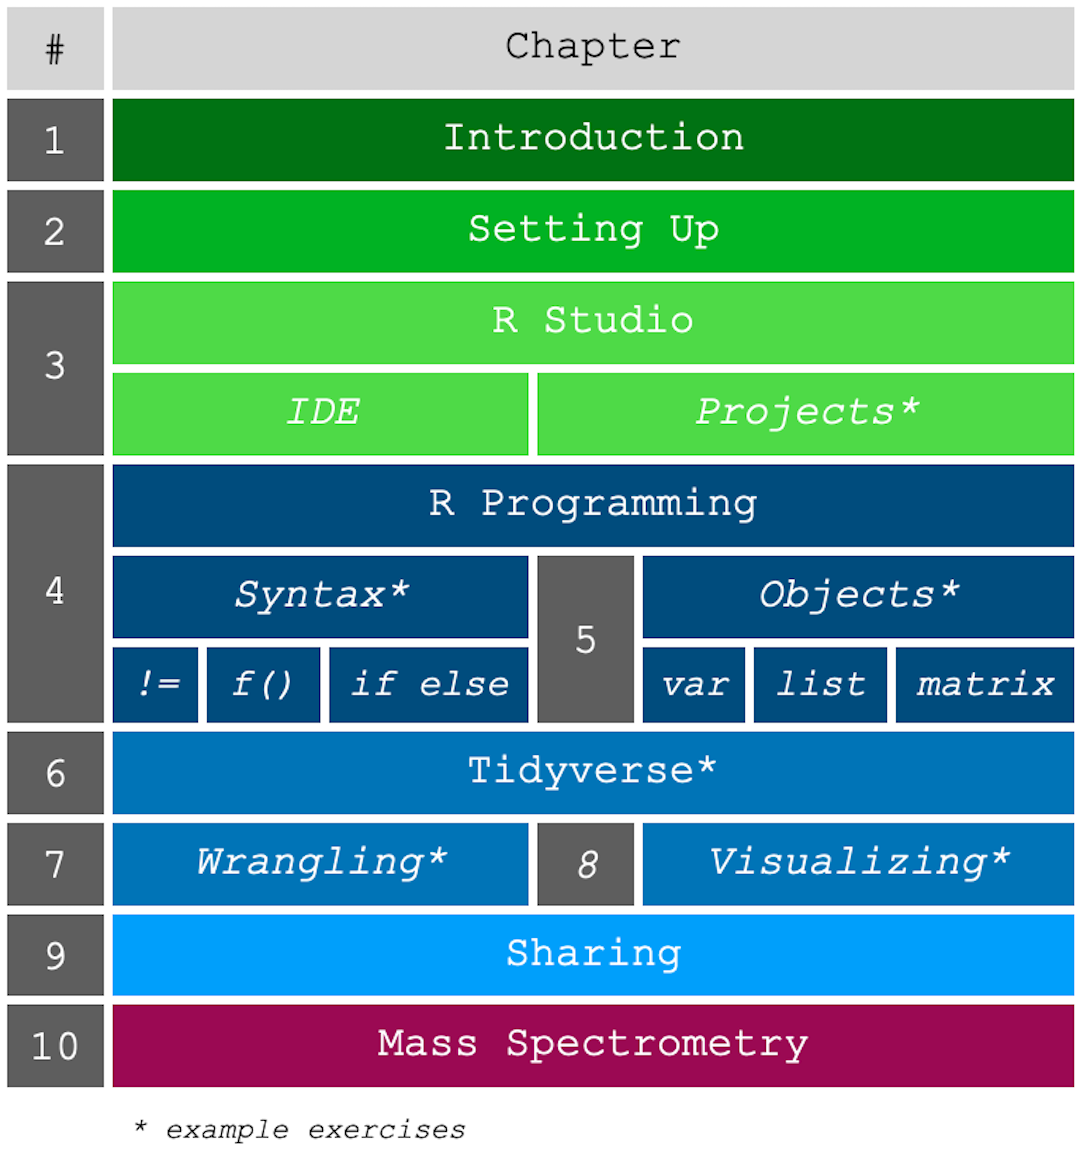
\includegraphics[width=15in]{images/01_000_book_contents} \end{center}

\hypertarget{introduction-to-r}{%
\chapter{Introduction to R}\label{introduction-to-r}}

Before we get started, this book contains some basic cues to help facilitate your understanding of the current topic.

\hfill\break

\begin{longtable}[]{@{}
  >{\raggedright\arraybackslash}p{(\columnwidth - 2\tabcolsep) * \real{0.2411}}
  >{\raggedright\arraybackslash}p{(\columnwidth - 2\tabcolsep) * \real{0.7589}}@{}}
\toprule\noalign{}
\endhead
\bottomrule\noalign{}
\endlastfoot
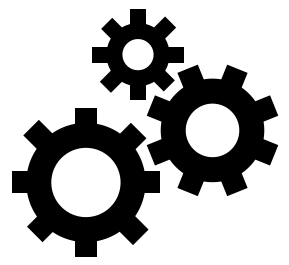
\includegraphics[width=\textwidth,height=0.70833in]{images/03.png} & \begin{minipage}[t]{\linewidth}\raggedright
\textbf{At the end of this chapter you should be able to}

\begin{itemize}
\item
  Understand why R is a good choice for data analysis.
\item
  Realize that you have just started the learning curve and all your efforts hence forth are worth it.
\item
  Know where to find additional educational resources.
\end{itemize}
\end{minipage} \\
\end{longtable}

\hfill\break

\hypertarget{why-choose-it}{%
\section*{Why choose it?}\label{why-choose-it}}
\addcontentsline{toc}{section}{Why choose it?}

In recent years, R has gained a lot of popularity among data scientists and analysts. The reason for this is simple: R is a language that is specifically designed for working with data. While other programming languages like C/C++, Java, and Python are general purpose languages that can be used in any domain, R is geared towards data analysis and manipulation.

Because R is designed for working with data, it has several features that make it easier to work with large datasets. For instance, R has several built-in data structures that allow users to organize and manipulate data in a variety of ways. Additionally, R has a wide range of libraries and packages that can be used to perform specific tasks like data visualization, statistical analysis, and machine learning.

Another reason why R is so popular among data scientists is that it is an open-source language. This means that anyone can contribute to its development, and there is a vast community of users and developers working together to improve the language and its capabilities.

Despite its many advantages, R does have a few limitations. For example, it is not as fast as some other programming languages, and it can be difficult for beginners to learn. However, there are many resources available online to help users learn R, and once they get the hang of it, they will find that it is a powerful tool for data analysis and visualization.

Overall, R is an excellent language for anyone who wants to work with data. Its specialized features and wide range of capabilities make it a top choice for data scientists and analysts everywhere.

The Stack Overflow blog post \href{https://stackoverflow.blog/2017/10/10/impressive-growth-r/}{The Impressive Growth of R} by David Robinson, discusses the growth and popularity of the programming language R. The post highlights the increase in R's usage on Stack Overflow, as well as the growing interest in R from various industries.

\begin{quote}
We found in a previous post that Python has a solid claim to being the fastest-growing programming language in terms of Stack Overflow visits. The same analysis showed that the R programming language has shown remarkable growth in the last five years as well. In fact, R is growing at a similar rate to Python\ldots{}
\end{quote}

The post provides an overview of R's history, its advantages and disadvantages, and its current position in the programming world. The author notes that R's popularity is due to its ability to handle large datasets, its flexibility for data analysis and in increase in popularity of data science and the growing number of companies using R for data analysis. Overall, the post concludes that R's growth and popularity are likely to continue in the future, as more industries recognize the value of data analysis and turn to R as a solution.

\hypertarget{what-you-can-do-with-it}{%
\section*{What you can do with it?}\label{what-you-can-do-with-it}}
\addcontentsline{toc}{section}{What you can do with it?}

The potential of what you can achieve with R is vast and ultimately depends on the level of dedication you have towards learning and expanding your skill set. By utilizing R, you can analyze data through various methods such as reading and plotting data, constructing analysis pipelines, prototyping new algorithms, and even writing your analysis code into shareable packages. With these abilities, you can not only perform data analysis, but also create a more efficient and reproducible workflow. The more you learn and experiment with R, the more you can discover and unlock its full potential.

\hfill\break

\begin{longtable}[]{@{}
  >{\raggedright\arraybackslash}p{(\columnwidth - 2\tabcolsep) * \real{0.2061}}
  >{\raggedright\arraybackslash}p{(\columnwidth - 2\tabcolsep) * \real{0.7939}}@{}}
\toprule\noalign{}
\endhead
\bottomrule\noalign{}
\endlastfoot

\includegraphics[width=\textwidth,height=0.70833in]{images/01.png} & \textbf{NOTES} Some helpful explanatory notes and tips appear as a block quote. \textbar{}
\textbar{}
- R can be a fast, nimble, forgiving scripting language with lots of ready-made tools and resources (CRAN, Github, Bioconductor). \\
\end{longtable}

\hfill\break

\hypertarget{the-r-learning-curve}{%
\section*{The R Learning Curve}\label{the-r-learning-curve}}
\addcontentsline{toc}{section}{The R Learning Curve}

The learning curve for R 10+ years ago was difficult as there where fewer R resources, it was less mature with not a lot of interest. Additionally, there were fewer people in the community and data science wasn't ``a thing'' yet.

\begin{figure}

{\centering 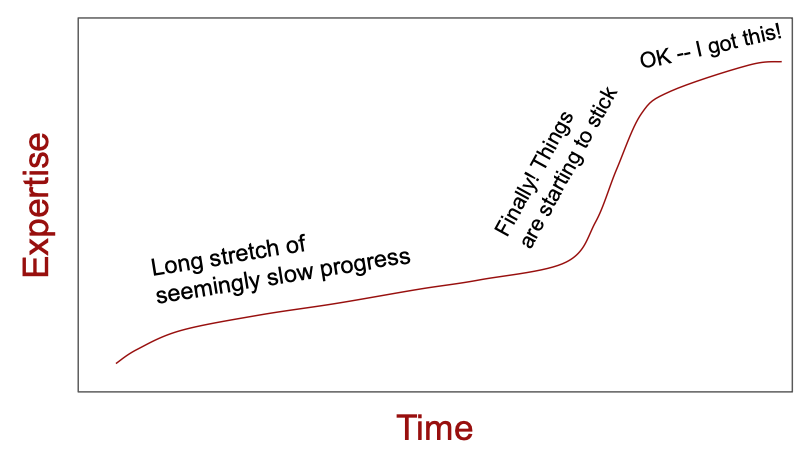
\includegraphics[width=11.21in]{images/01_001_r_learning_curve_past} 

}

\caption{\label{fig:1001}R learning curve past}\label{fig:1001}
\end{figure}

The R programming language is still challenging but worth it. With the introduction of packages encompassed in the tidyverse there are more high-quality resources, mature utilization with well documented explanations and examples. Currently there is lots of current interest in R with a large community of users and developers. Additionally, the data science ``revolution has pushed R to develop and evolve, become more user-centric.

\begin{figure}

{\centering 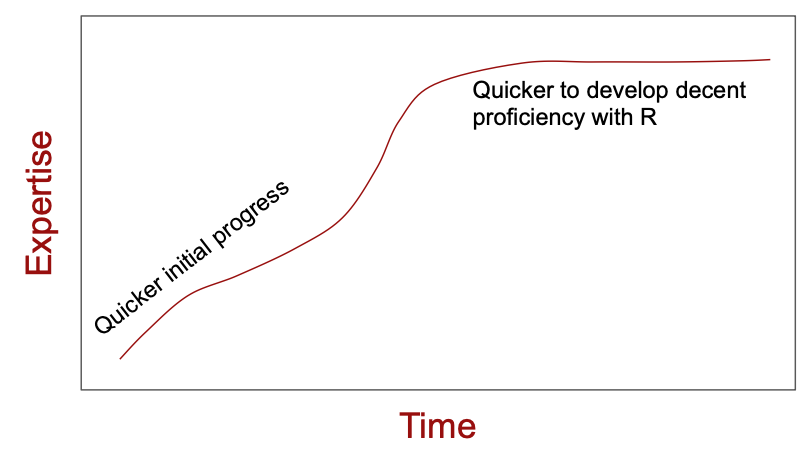
\includegraphics[width=11.21in]{images/01_002_r_learning_curve_present} 

}

\caption{\label{fig:1002}R learning curve present}\label{fig:1002}
\end{figure}

\hypertarget{thoughts-about-learning-r-and-how-to-code}{%
\section*{Thoughts about learning R and how to code}\label{thoughts-about-learning-r-and-how-to-code}}
\addcontentsline{toc}{section}{Thoughts about learning R and how to code}

When it comes to learning a programming language, it can be daunting to know where to start. However, the first step to learning any programming language is to understand its syntax. Syntax refers to the set of rules and symbols that make up structurally correct code. Without proper syntax, even the smallest of errors can result in code that doesn't run. These errors could be as simple as a typo, an incorrect name, missing spaces or too many spaces, or even wrong brackets. Syntax errors can be frustrating, especially for beginners, but it's important to hang in there and start simple.

It's best to begin by trying to understand very simple cases first, before building and expanding on them. This approach will help you to get a better grip on the basics of the language and will help you to avoid becoming overwhelmed. If you're learning R, there are many resources available to help you get started. You could start by reading through the R Book, which provides a comprehensive guide to the R programming language. Alternatively, there are many online tutorials available, which can help to break down complex concepts into more manageable pieces.

In short, when learning R, it's important to remember that syntax is key. By taking the time to understand the syntax rules, you can avoid frustrating syntax errors and build a solid foundation for your future coding endeavors

\hypertarget{alternatives}{%
\section*{Alternatives}\label{alternatives}}
\addcontentsline{toc}{section}{Alternatives}

When it comes to data science, R is a popular programming language among statisticians and data analysts. However, there are several data science alternatives to R that are also gaining popularity.

One of the most popular alternatives to R is Python. Python is a general-purpose programming language that has a wide range of libraries and frameworks for data science. It is known for its simplicity, readability, and versatility. Python's libraries such as NumPy, Pandas, and Scikit-Learn are widely used in data science for tasks such as data cleaning, data analysis, and machine learning.

Another alternative to R is Julia, a new programming language that is designed specifically for scientific computing and numerical analysis. Julia is known for its speed and efficiency, making it a great choice for data analysis and modeling. Julia also has a growing package ecosystem with libraries such as DataFrames.jl and Flux.jl that are specifically designed for data science.

Matlab is another alternative to R that is widely used in the scientific community. Matlab is known for its extensive numerical computing capabilities and its strong visualization features. It is commonly used in fields such as engineering, physics, and finance for data analysis and modeling.

In conclusion, while R is a popular language for data science, it is not the only option available. Python, Julia, and Matlab are all viable alternatives with their own strengths and weaknesses. It is important to consider the specific needs of your project and choose the programming language that best suits your requirements.

\textbf{Did you know}, that while R on its own is a powerful scripting language, some analytical tasks might require the use of other programming languages such as Python, C++ or Rust. Luckily, R provides different packages that allow us to use these languages within R code. These packages provide a seamless integration between these languages and R, allowing you to leverage the strengths of each language to perform complex tasks.

The \texttt{reticulate} package enables the integration of Python code in R. This package allows you to import Python modules and functions directly into R and also allows you to call Python functions from R code. This is especially useful when you need to use Python's machine learning libraries such as TensorFlow or PyTorch, which are not yet available in R.

Similarly, the \texttt{Rcpp} package provides a smooth integration between R and C++. With this package, you can easily write C++ functions and use them directly in your R code. This is useful when you need to perform computationally-intensive tasks, such as simulations or optimization, that require the speed of C++.

Finally, the \texttt{extendr} package provides an interface between R and Rust, allowing you to use Rust functions in R code and vice versa. Rust is a relatively new programming language that provides a balance between performance and safety. It is especially useful when you need to develop high-performance and low-level code, such as in systems programming or hardware development.

\hypertarget{resources}{%
\section*{Resources}\label{resources}}
\addcontentsline{toc}{section}{Resources}

When working with R, it is important to understand the basics and terms so that you can ask the right questions when seeking help. In the next two sections, we will provide an overview of these concepts to ensure that you have a solid foundation. It is worth noting that while googling your issue can be a great starting point, it is also important to seek out additional resources to help you solve your problem. For instance, you might consider joining an R community or forum where you can ask questions and receive feedback from other users. Additionally, many universities and organizations offer R workshops or training programs that can help you build your skills and knowledge. By taking advantage of these resources, you can develop a deeper understanding of R and become more confident in your ability to use it for data analysis and visualization.

\hypertarget{online}{%
\subsection*{Online}\label{online}}
\addcontentsline{toc}{subsection}{Online}

In addition to Googling to find how to do something in R, there are several online resources available for individuals learning R programming and needing assistance with concepts or coding issues. These resources include CRAN, Bioconductor, RStudio Community, R-bloggers, and Stack Overflow. Each of these resources offers different benefits, such as packages, forums, blogs, and Q\&A communities, to help R users.

\hypertarget{locating-available-packages-pre-built-algorithms}{%
\subsubsection*{Locating available packages (pre-built algorithms)}\label{locating-available-packages-pre-built-algorithms}}
\addcontentsline{toc}{subsubsection}{Locating available packages (pre-built algorithms)}

\begin{itemize}
\item
  The Comprehensive R Archive Network: \href{https://cran.r-project.org/}{cran.r-project.org/}
\item
  Bioconductor: \href{https://bioconductor.org/}{bioconductor.org/}
\end{itemize}

\hypertarget{ways-to-ask-for-help-or-find-answers-to-a-similar-question}{%
\subsubsection*{Ways to ask for help, or find answers to a similar question}\label{ways-to-ask-for-help-or-find-answers-to-a-similar-question}}
\addcontentsline{toc}{subsubsection}{Ways to ask for help, or find answers to a similar question}

\begin{itemize}
\item
  The RStudio Community: \href{https://community.rstudio.com/}{community.rstudio.com/}
\item
  R Community Explorer: \href{https://r-community.org/rstudio/}{r-community.org/rstudio/}
\item
  R bloggers: \href{https://www.r-bloggers.com/}{r-bloggers.com/}
\item
  Stack Overflow: \href{https://stackoverflow.com/questions/tagged/r}{stackoverflow.com/}
\end{itemize}

\hypertarget{more-ways-to-search-and-find-what-you-are-looking-for}{%
\subsubsection*{More ways to search and find what you are looking for}\label{more-ways-to-search-and-find-what-you-are-looking-for}}
\addcontentsline{toc}{subsubsection}{More ways to search and find what you are looking for}

\begin{itemize}
\item
  R-Seek: \href{https://rseek.org/}{rseek.org/}
\item
  R-universe: \href{https://r-universe.dev/search/}{r-universe.dev/search/}
\end{itemize}

\hypertarget{cheat-sheets}{%
\subsubsection*{Cheat-sheets}\label{cheat-sheets}}
\addcontentsline{toc}{subsubsection}{Cheat-sheets}

\begin{itemize}
\item
  Tidyverse: \href{https://www.tidyverse.org/}{www.tidyverse.org/}

  \begin{itemize}
  \item
    reading data: \href{https://readr.tidyverse.org/}{readr.tidyverse.org/}
  \item
    manipulating data :\href{https://dplyr.tidyverse.org/}{dplyr.tidyverse.org/}
  \item
    arranging table data: \href{https://tidyr.tidyverse.org/}{tidyr.tidyverse.org/}
  \item
    visualizing data \href{https://ggplot2.tidyverse.org/}{ggplot2.tidyverse.org/}
  \item
    working with strings: \href{https://stringr.tidyverse.org/}{stringr.tidyverse.org/}
  \item
    working with date and time: \href{https://lubridate.tidyverse.org/}{lubridate.tidyverse.org/}
  \end{itemize}
\end{itemize}

\hypertarget{in-print}{%
\subsection*{In Print}\label{in-print}}
\addcontentsline{toc}{subsection}{In Print}

R books in print are becoming increasingly popular due to the growing demand for R programming and data analysis. These books offer several benefits that make them an excellent resource for anyone who wants to learn R programming or improve their data analysis skills. One of the key advantages of R books in print is that they are easy to read and navigate. The authors of these books take into consideration that not everyone who reads their books is an expert in programming. They use simple language and examples to explain concepts from the basics, making it easy for readers to understand. They can be used as a quick reference guide when working on a project or when facing a programming challenge. R books in print are cost-effective. While online resources are free, they are not always reliable, and it can be time-consuming to find the information you need. R books in print, on the other hand, are written and edited by experts who have years of experience in the field making them a reliable source of information.

\begin{center}\rule{0.5\linewidth}{0.5pt}\end{center}

\textbf{R for Data Science: Import, Tidy, Transform, Visualize, and Model Data 1st Edition} \emph{by Garrett Grolemund, Hadley Wickham}

\begin{quote}
Learn how to use R to turn raw data into insight, knowledge, and understanding.
This book introduces you to R, RStudio, and the tidyverse, a collection of R
packages designed to work together to make data science fast, fluent, and fun.
Suitable for readers with no previous programming experience, R for Data
Science is designed to get you doing data science as quickly as possible.
\end{quote}

\begin{center}\rule{0.5\linewidth}{0.5pt}\end{center}

\textbf{Use R!}, a collection of 67 print books.

The Use R! collection of print books is a series of books aimed at helping people learn and use the R programming language. The books in this series cover a wide range of topics related to R, including data analysis, statistical modeling, and data visualization.

Each book in the collection is written by a different author or group of authors, and provides a unique perspective on how to use R for different tasks. The books are targeted at a range of audiences, from beginners who are just starting to learn R, to more advanced users who are looking to expand their skills and knowledge.

Some of the popular books in the Use R! collection include:

\begin{itemize}
\tightlist
\item
  \textbf{An Introduction to R} by Venables and Smith: This book provides a comprehensive introduction to the R programming language, covering topics such as data types, control structures, and functions.
\item
  \textbf{Data Manipulation with R} by Spector: This book covers how to use R to manipulate data, including topics such as data cleaning, merging, and reshaping.
\item
  \textbf{ggplot2: Elegant Graphics for Data Analysis} by Wickham: This book provides an in-depth introduction to the ggplot2 package in R, which is used for creating high-quality data visualizations.
\item
  \textbf{Applied Regression Analysis} by Fox: This book covers how to use R to perform regression analysis, including topics such as linear regression, logistic regression, and mixed-effects models.
\end{itemize}

In summary, the Use R! collection of print books is a valuable resource for anyone looking to learn or improve their skills in the R programming language. With a wide range of topics and authors, there is something for everyone in this collection.

\hypertarget{organizations}{%
\subsection*{Organizations}\label{organizations}}
\addcontentsline{toc}{subsection}{Organizations}

Many R organizations offer individuals an opportunity for training and support, networking, access to resources, and help building a reputation. These benefits make R organizations a valuable resource to consider for both individuals and organizations using R for statistical computing and graphics.

\hfill\break

\begin{longtable}[]{@{}
  >{\raggedright\arraybackslash}p{(\columnwidth - 2\tabcolsep) * \real{0.2615}}
  >{\raggedright\arraybackslash}p{(\columnwidth - 2\tabcolsep) * \real{0.7385}}@{}}
\toprule\noalign{}
\endhead
\bottomrule\noalign{}
\endlastfoot

\includegraphics[width=\textwidth,height=0.70833in]{images/01.png} & \textbf{R User Group (RUG)}

RUGs are a relaxed and friendly way to broaden your contacts, scope and understanding of R. \textbar{} \\
\end{longtable}

\hfill\break

\hypertarget{r-user-groups}{%
\subsubsection*{R User Groups}\label{r-user-groups}}
\addcontentsline{toc}{subsubsection}{R User Groups}

R User Groups are communities of people who are interested in using R, a programming language and software environment for statistical computing and graphics. These groups are formed to provide a platform for individuals to learn, share knowledge, and collaborate on projects related to R programming.

R User Groups usually meet on a regular basis, either virtually or in person, and organize events such as talks, workshops, and hackathons. These events are designed to provide members with opportunities to improve their skills, network with like-minded individuals, and work on projects that are of mutual interest.

R User Groups are open to anyone who is interested in using R, regardless of their level of expertise. Members can range from beginners who are just starting to learn R, to experienced professionals who use R on a daily basis. This diversity of membership allows for a rich exchange of ideas and perspectives on the use of R in various fields, such as data science, finance, and healthcare.

Joining an R User Group can be a great way to stay up-to-date with the latest developments in R programming, as well as to learn from and collaborate with other members. Many R User Groups also have online forums or discussion boards where members can ask questions, share resources, and seek feedback on their work.

\textbf{Where to find a RUG}

\begin{itemize}
\item
  \href{https://r-community.org/usergroups/}{R Community}
\item
  \href{https://jumpingrivers.github.io/meetingsR/r-user-groups.html}{Another list of RUGs}\\
\end{itemize}

\hypertarget{r-specific-confrences}{%
\subsubsection*{R Specific Confrences}\label{r-specific-confrences}}
\addcontentsline{toc}{subsubsection}{R Specific Confrences}

\href{https://rstats.ai/gov}{The R Confrence}

The \emph{R Conference} currently takes place in New York, Washington D.C., and soon Dublin, Ireland. They were created to foster the local R communities and serve as gathering places for people to learn from their peers. The \emph{R Conference} hosts one of the most elite gatherings of data scientists and data professionals who come together to explore, share, inspire and to promote the growth of open source ideals.

\href{https://d4con.io/}{D4 Confrence}

\emph{Innovation and Entrepreneurship in Data, Design, Development and Discovery}

The D4 conference exists to bring creative communities together and to bolster the exchange of ideas. Data professionals, software developers, and other creatives can meet and collaborate.

\hypertarget{r-education-at-confrences}{%
\subsubsection*{R Education at Confrences}\label{r-education-at-confrences}}
\addcontentsline{toc}{subsubsection}{R Education at Confrences}

\href{https://ASMS.org/}{ASMS}

\emph{American Society for Mass Spectrometry}

The American Society for Mass Spectrometry (ASMS) was created in 1969 to promote and share knowledge of mass spectrometry. Membership includes over 8,500 scientists from academia, industry, and government labs. Members focus on technique and instrument advancements, as well as research in various sciences. ASMS offers several short-courses (1 or 2-day) covering a myriad of topics, including using R for data analysis.

\href{https://www.msacl.org/}{MSACL}

\emph{Mass Spectrometry \& Advances in the Clinical Lab}

MSACL aims to advance mass spectrometry and other advanced technologies in clinical laboratory medicine through education and training of practitioners, physicians, and other healthcare professionals. They also support the development of new technologies for diagnosis, treatment, and prognosis of clinical disorders. MSACL offers resources through their Learning Center on several topics, including using R in clinical data analysis.

\hypertarget{installation}{%
\chapter{Installation}\label{installation}}

In the scope of this book, there are three main components that need to be installed, and periodically updated:

\begin{itemize}
\item
  \textbf{The R interpreter} - the software that understands math and plotting
\item
  \textbf{RStudio IDE} - the software that makes it easy write code and visualize data
\item
  \textbf{R Packages} - bits of R code that perform specalized operations
\end{itemize}

In this book we will be utilizing the RStudio integrated development environment (IDE) to interact with R. Two separate components are required for this - the R interpreter and the RStudio IDE. Both are required as the RStudio IDE only provides an interface for the R interpreter, which reads the code and does all the mathematical operations. The R interpreter can be used alone, interacting through the command line (eg. Windows CMD, MacOS and Linux Terminal), a plain text editor or another IDE such as Xcode, VSCode, Eclipse, Notepad++, etc. Rstudio provides a comprehensive, R specific environment, with auto-complete, code syntax highlighting, in-editor function definitions along with package management and plot visualizations.

\hfill\break

\begin{longtable}[]{@{}
  >{\raggedright\arraybackslash}p{(\columnwidth - 2\tabcolsep) * \real{0.3656}}
  >{\raggedright\arraybackslash}p{(\columnwidth - 2\tabcolsep) * \real{0.6344}}@{}}
\toprule\noalign{}
\endhead
\bottomrule\noalign{}
\endlastfoot
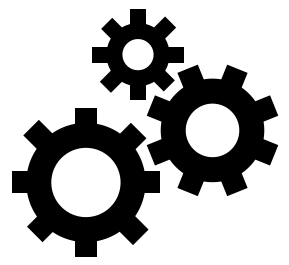
\includegraphics[width=\textwidth,height=0.70833in]{images/03.png} & \begin{minipage}[t]{\linewidth}\raggedright
\textbf{At the end of this chapter you should be able to}

\begin{enumerate}
\def\labelenumi{\arabic{enumi}.}
\item
  Install R, RStudio and a few R packages
\item
  Understand the major components for working with R.
\end{enumerate}
\end{minipage} \\
\end{longtable}

\hfill\break

\hypertarget{r-interpreter}{%
\section{R interpreter}\label{r-interpreter}}

The underlying ``engine'' for R programming language can be downloaded from \href{https://www.r-project.org/}{The R Project for Statistical Computing}. R is an open-source implementation of the S statistical computing language originally developed at Bell Laboratories. Both langauges contain a variety of statistical and graphical techniques, however, R has been continually extended by professional, academic and amateur contributors and remains the most active today. With the advent of open-source sharing platforms such as GitHub, R has become increasingly popular among data scientists because of its ease of use and flexibility in handling complex analyses on large datasets. Additionally, one of R's strengths is the ease with which well-designed publication-quality plots can be produced.

\hypertarget{steps}{%
\subsubsection*{Steps}\label{steps}}
\addcontentsline{toc}{subsubsection}{Steps}

\begin{enumerate}
\def\labelenumi{\arabic{enumi}.}
\tightlist
\item
  Navigate to \href{https://www.r-project.org/}{The R Project}
\item
  Click on \href{https://cran.r-project.org/mirrors.html}{CRAN} under Download, left-hand side
\item
  Click on \url{https://cloud.r-project.org/} under 0-Cloud\\
  \emph{This will take you to the globally nearest up-to-date repository}
\item
  Click on \texttt{Download\ for\ ...} and choose the OS compatible with your device
\end{enumerate}

\hypertarget{windows-os}{%
\subsubsection*{Windows OS}\label{windows-os}}
\addcontentsline{toc}{subsubsection}{Windows OS}

Click on \texttt{base}

\hypertarget{macos}{%
\subsubsection*{MacOS}\label{macos}}
\addcontentsline{toc}{subsubsection}{MacOS}

\textbf{For an Intel CPU}: click \texttt{R-4.x.x.pgk} to download\\
\textbf{For an M1 CPU}: click \texttt{R-4.x.x-arm64.pkg} to download

After downloading, double-click the installer and follow the instructions

\begin{figure}
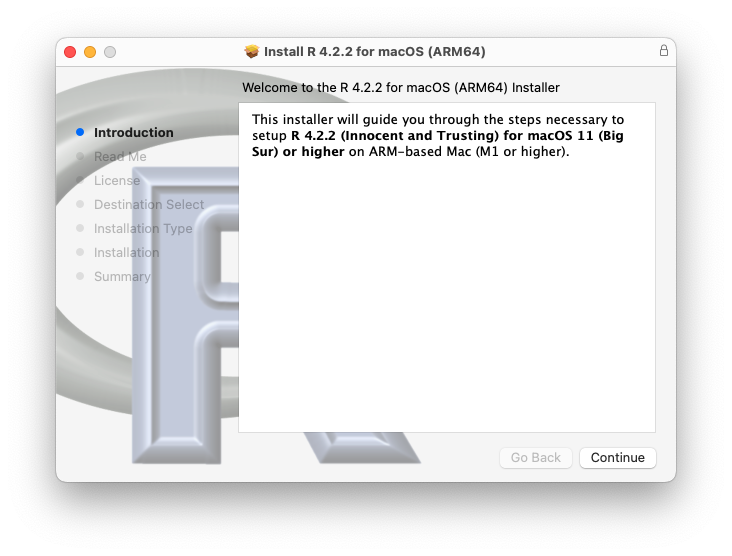
\includegraphics[width=10.17in]{images/02_001_r_installer_mac_m1} \caption{\label{fig:2001}Mac Installer}\label{fig:2001}
\end{figure}

\hypertarget{linux}{%
\subsubsection*{Linux}\label{linux}}
\addcontentsline{toc}{subsubsection}{Linux}

Click on your distribution and follow the instructions provided. Most of these instructions require knowledge of the Terminal and command line interface for *unix systems.

\hypertarget{rstudio}{%
\section{Rstudio}\label{rstudio}}

RStudio, prior to 2023, was an independent software provider for the ever-popular RStudio products, which included both the desktop and server based IDEs, along with the RShiny applications and servers that facilitate easy-to-build interactive web applications straight from R, and deployed on the web. The last chapter in this book will explore the \texttt{tidyproteomics} package which also has a Shiny web application. RStudio announced at the beginning of 2023 a soft pivot to Posit, which essentially is a rebranding of the RStudio company to encompass a larger data science audience, one that also provides integration with the Python programming language inside the RStudio IDE.

\begin{quote}
The most trusted IDE for open source data science

``RStudio is an integrated development environment (IDE) for R and Python. It includes a console, syntax-highlighting editor that supports direct code execution, and tools for plotting, history, debugging, and workspace management. RStudio is available in open source and commercial editions and runs on the desktop (Windows, Mac, and Linux).''

--- www.posit.co (Jan 2023)
\end{quote}

\hypertarget{steps-1}{%
\subsubsection*{Steps}\label{steps-1}}
\addcontentsline{toc}{subsubsection}{Steps}

\begin{enumerate}
\def\labelenumi{\arabic{enumi}.}
\tightlist
\item
  Navigate to \href{https://posit.co/}{posit.co}, alternatively \href{https://rstudio.com/}{rstudio.com} redirects to the Posit website.
\item
  \textbf{Click} \texttt{Download\ RStudio} in the menu top right
\item
  Select \texttt{RStudio\ Desktop}
\item
  \textbf{Click} \texttt{Download\ RStudio}\\
  \emph{skip 1: Install R}
\item
  \textbf{Click} \texttt{Download\ RStudio\ Desktop\ for\ ..}
\end{enumerate}

\hypertarget{windows-os-1}{%
\paragraph*{Windows OS}\label{windows-os-1}}
\addcontentsline{toc}{paragraph}{Windows OS}

\hypertarget{macos-1}{%
\paragraph*{MacOS}\label{macos-1}}
\addcontentsline{toc}{paragraph}{MacOS}

Opening the .dmg file shows the archive that can be copied into the Applications folder simply by click-dragging the application onto the Applications folder shortcut.

\begin{figure}
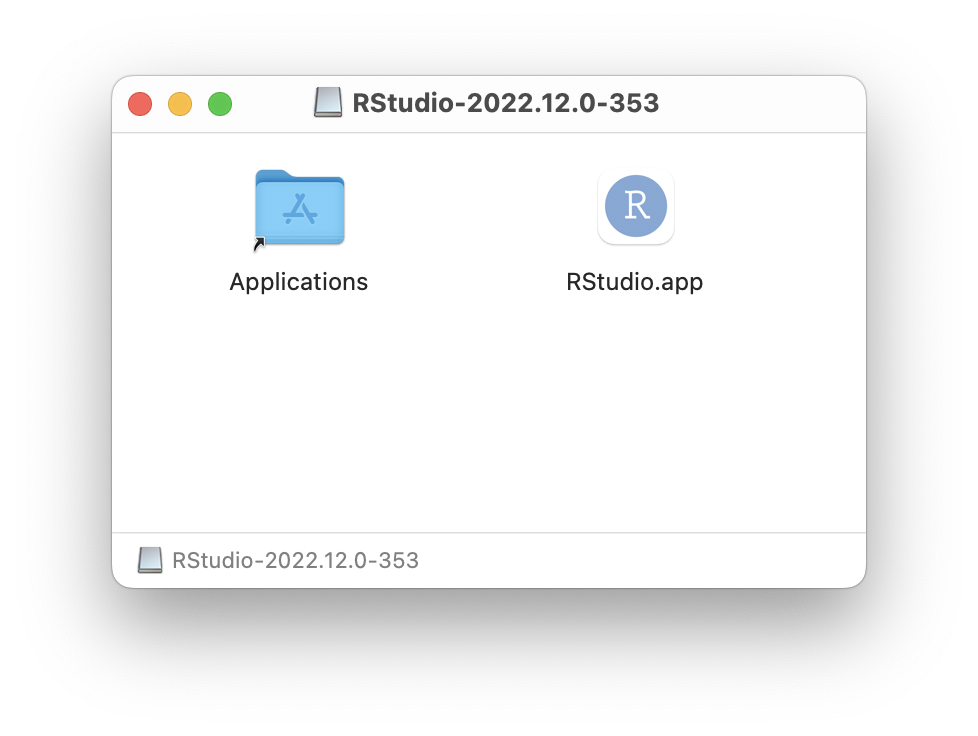
\includegraphics[width=13.58in]{images/02_011_rstudio_installer_mac} \caption{\label{fig:2011}RStudio IDE Install}\label{fig:2011}
\end{figure}

\hypertarget{linux-1}{%
\paragraph*{Linux}\label{linux-1}}
\addcontentsline{toc}{paragraph}{Linux}

\hypertarget{ide-layout}{%
\subsection{IDE Layout}\label{ide-layout}}

The RStudio Integrated Development Environment (IDE) is a powerful tool that can make your data analysis and coding tasks more manageable. One of the key features of the RStudio IDE is that it consists of four individual panes, each containing parts of the total environment. This makes it easier for you to navigate your coding and analysis tasks.

For example, while creating and viewing a plot, you can have the text editor and console open and organized. This way, you can easily see how the code you are writing is impacting the plot you are creating. Having everything in one place can also help reduce the clutter on your desktop, as you don't need to have multiple applications open at the same time.

Overall, the RStudio IDE is an excellent option for anyone looking to streamline their coding and data analysis workflows. By taking advantage of its various features, you can make your work more efficient and enjoyable.

\begin{figure}
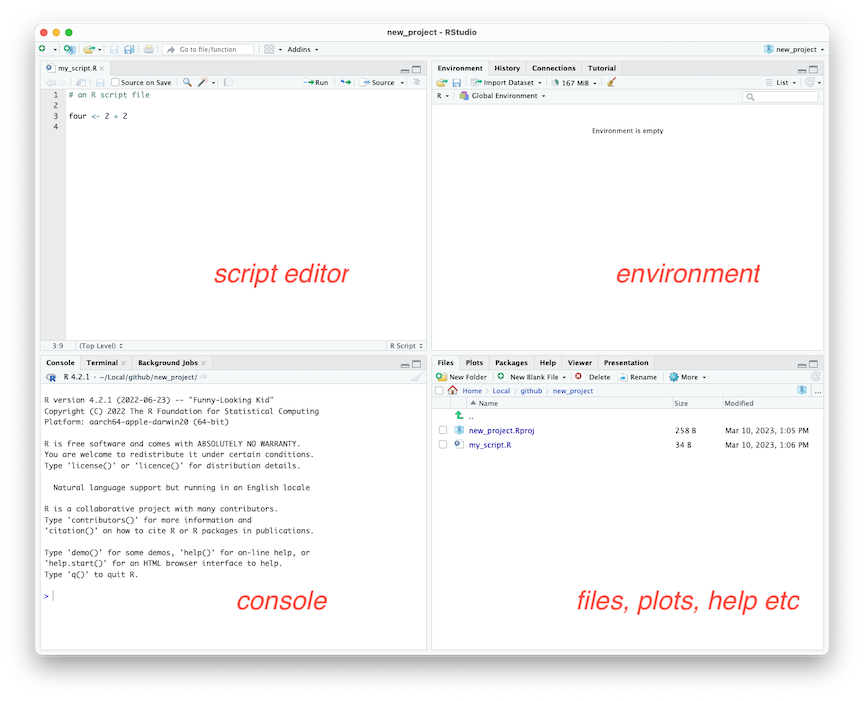
\includegraphics[width=19.19in]{images/02_021_rstudio_panes} \caption{\label{fig:2021}RStudio IDE in the default layout}\label{fig:2021}
\end{figure}

\hypertarget{the-editor}{%
\subsubsection*{The Editor}\label{the-editor}}
\addcontentsline{toc}{subsubsection}{The Editor}

\begin{quote}
\textbf{Tabs}: \texttt{All\ Open\ Files}
\end{quote}

The \emph{Editor} is a tool that allows you to write R code with ease. It is essentially a text editor, but with the added benefit of having knowledge of R. This means that it can automatically color different parts of your code based on their function. This can be a huge time saver, as it makes it easier to read and understand your code.

For example, comments in R code start with a hash (\#) symbol. In the \emph{Editor}, these comments are colored light green, making them easy to spot. Similarly, operators like the plus sign (+) and the assignment operator (\textless-) are colored light blue. This makes it easy to identify where these operators are being used in your code.

Variables are an important part of any programming language, and R is no exception. In the \emph{Editor}, variables are colored black. This makes it easy to distinguish variable names from other parts of your code. Finally, quoted text (also known as strings) are colored purple. This makes it easy to identify where strings are being used in your code.

In summary, the \emph{Editor} is a powerful tool that can help you write R code more efficiently. By automatically coloring different parts of your code, it makes it easier to read and understand. Whether you are a beginner or an experienced R programmer, the \emph{Editor} can help you write better code in less time.

\begin{figure}
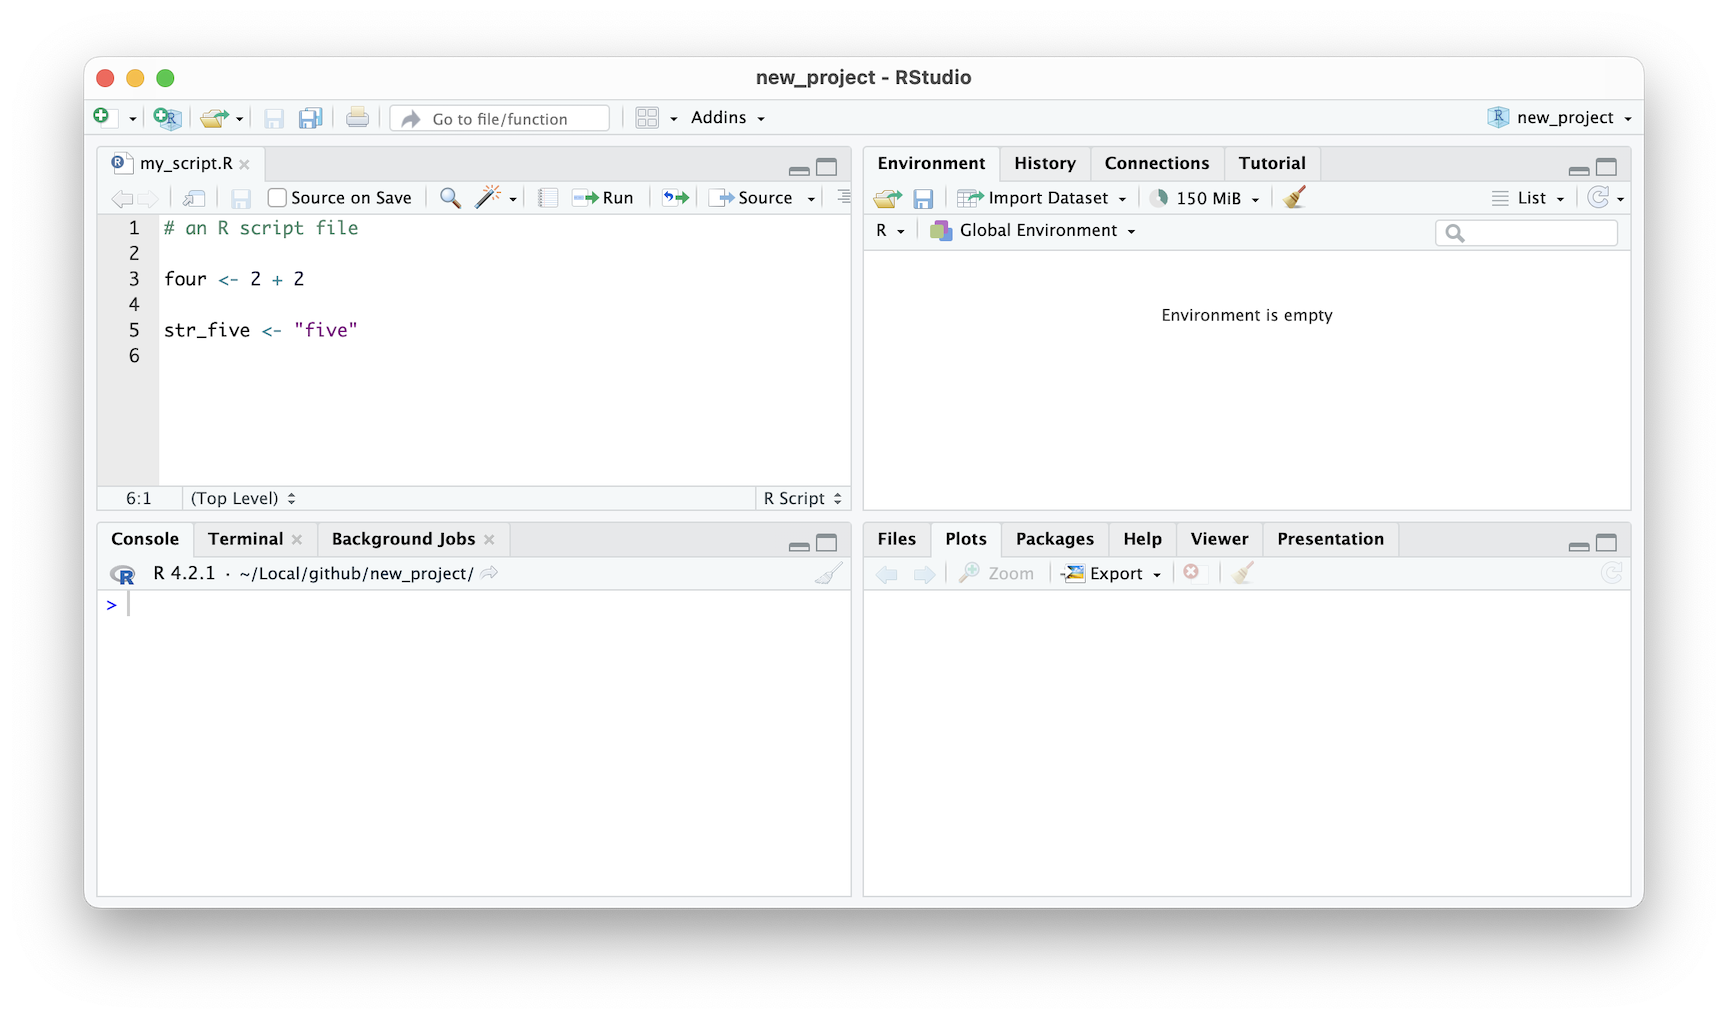
\includegraphics[width=31.94in]{images/02_022_editor_highlighting} \caption{\label{fig:2022}RStudio IDE syntax highlighting}\label{fig:2022}
\end{figure}

The Editor also has the ability to suggest available variables and functions. In the image provided, the editor suggests using the mean() function to calculate the average of a collection of values. A pop-up with a description accompanies the suggestion. This feature occurs after typing in the first three letters of anything, and the editor will try to guess what you want to type next. This is a helpful tool that can save you time and effort when writing R code.

\begin{figure}
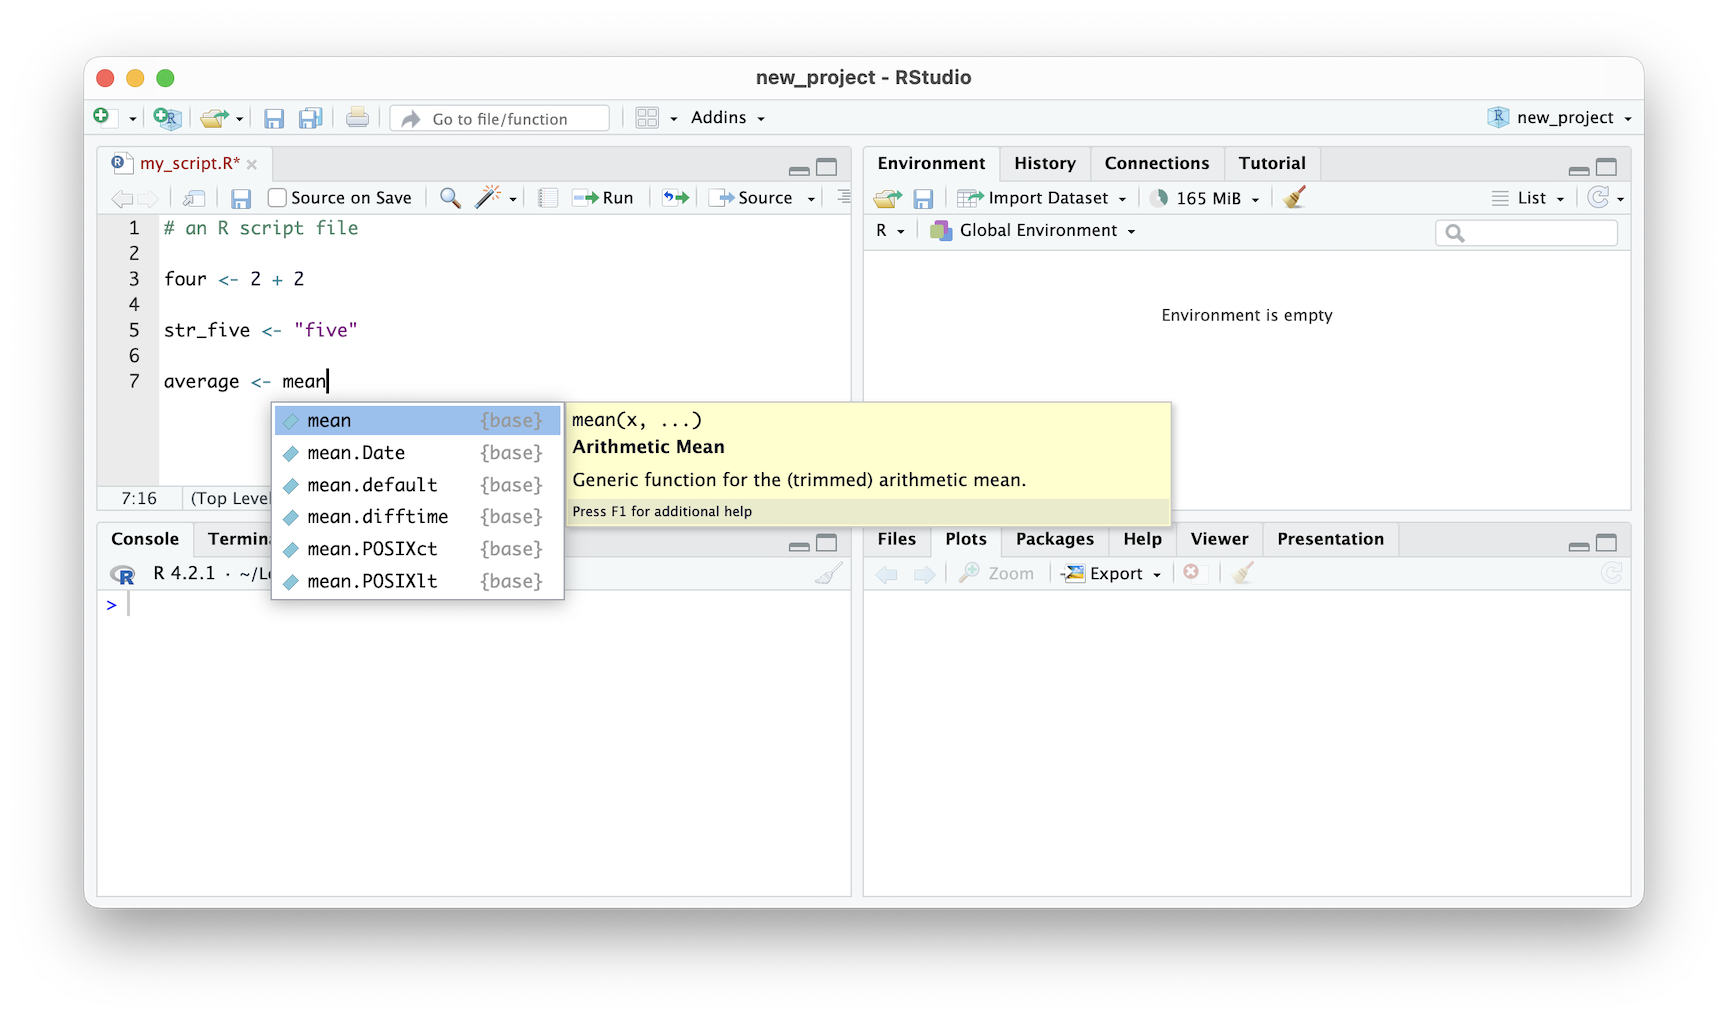
\includegraphics[width=31.94in]{images/02_023_editor_autocomplete} \caption{\label{fig:2023}RStudio IDE auto complete}\label{fig:2023}
\end{figure}

\hypertarget{files-and-plots}{%
\subsubsection*{Files and Plots}\label{files-and-plots}}
\addcontentsline{toc}{subsubsection}{Files and Plots}

\begin{quote}
\textbf{Tabs}: \texttt{Files}, \texttt{Plots}, \texttt{Packages}, \texttt{Viewer}, and \texttt{Presentation}
\end{quote}

When you're working in RStudio, your workflow is made simple with the various tabs and features available. For instance, the script that you're currently working on is saved to the current project and can be accessed via the \emph{Files} tab located on the top right-hand side of the pane. This tab provides an overview of all the files in the working directory, and you can easily navigate between them.

If you need to open another file, you can do so by clicking on the \emph{File} menu or by using the shortcut key. When you open a new file, it will create a new tab in the \emph{Editor} pane, which allows you to switch between open files. This feature is super helpful when you're working on multiple files simultaneously.

Another useful tab located in the same pane is the \emph{Plots} tab. This tab provides a quick way to view any active plots instantly. You don't need to export your plots or save them separately. Instead, you can view them right within RStudio. This is where RStudio truly shines, as it brings together editing and visualization in one application.

\begin{figure}
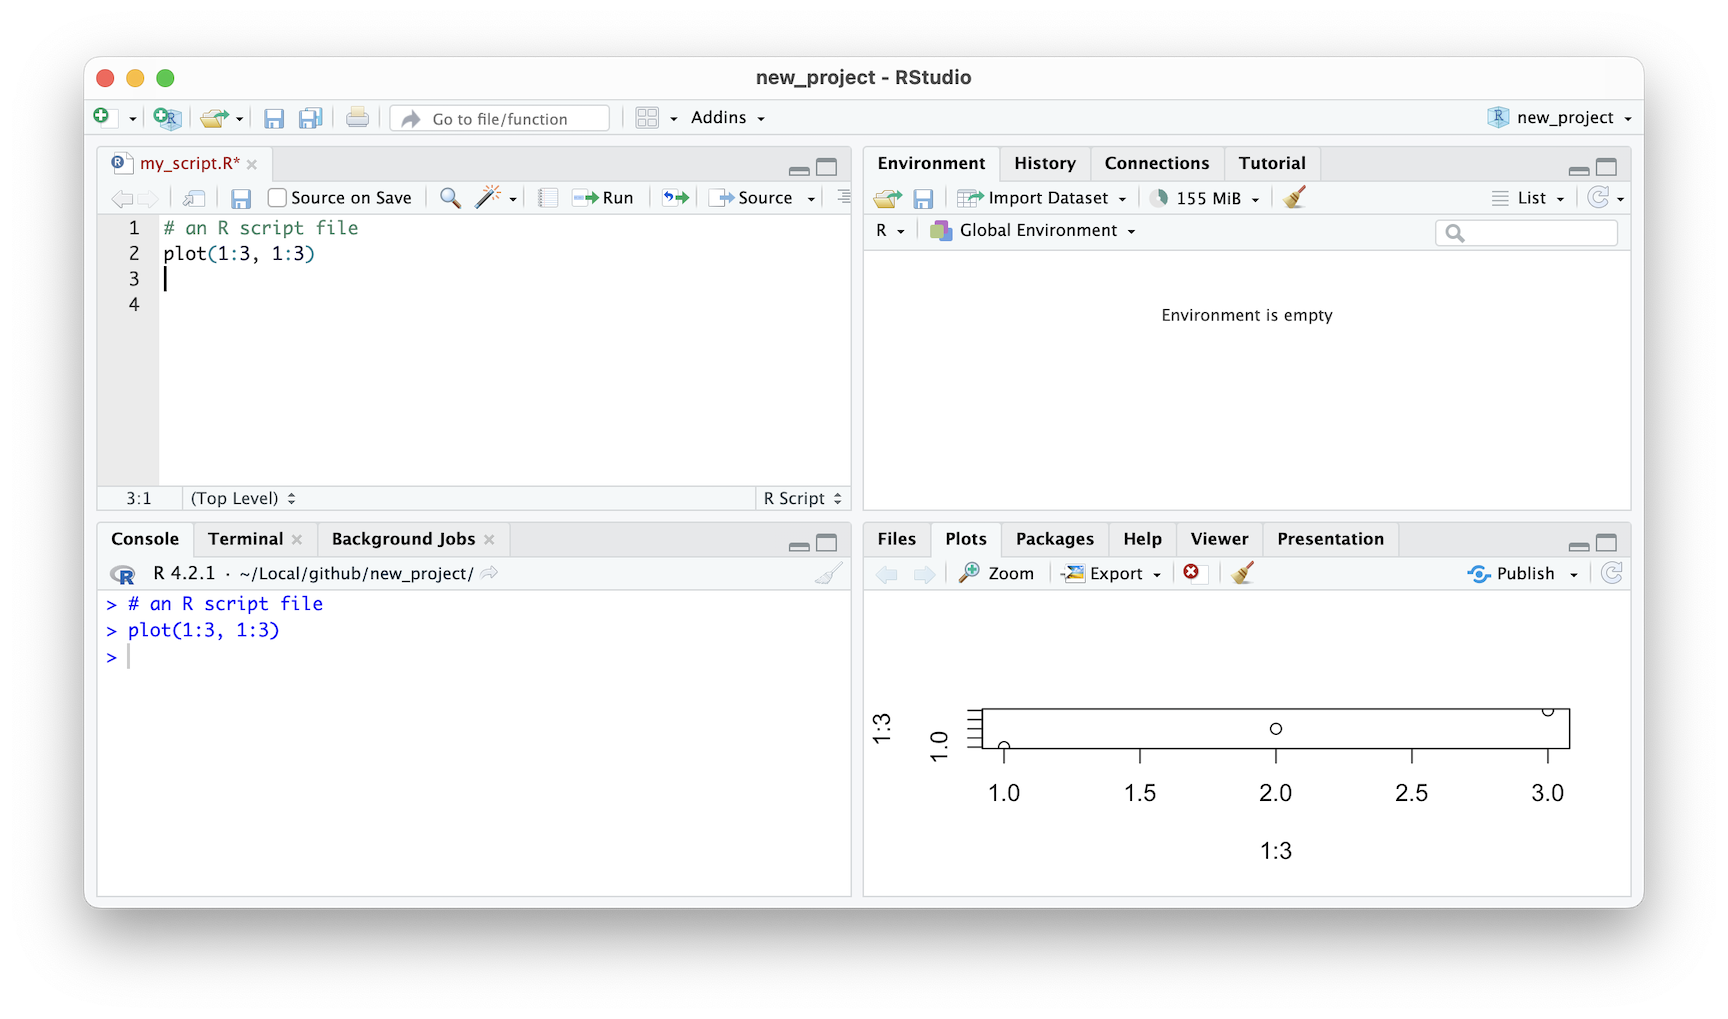
\includegraphics[width=31.94in]{images/02_024_qplot} \caption{\label{fig:2024}RStudio IDE plot window}\label{fig:2024}
\end{figure}

\hypertarget{the-console}{%
\subsubsection*{The Console}\label{the-console}}
\addcontentsline{toc}{subsubsection}{The Console}

\begin{quote}
\textbf{Tabs}: \texttt{Console}, \texttt{Terminal}, and \texttt{Background\ Jobs}
\end{quote}

In the RStudio IDE, the \emph{Console} pane is where lines of code are executed from the editor. It is a vital component of the RStudio interface that allows users to interact with R in real-time. The \emph{Console} pane is not only where code is run, but it is also where users can view output and error messages. Additionally, the \emph{Console} pane provides users access to the computer's terminal. This feature allows users to execute commands outside of the R environment, such as navigating files and directories or installing packages. Overall, the \emph{Console} pane is an essential tool for any RStudio user and should be utilized to its full potential.

\hypertarget{environment}{%
\subsubsection*{Environment}\label{environment}}
\addcontentsline{toc}{subsubsection}{Environment}

\begin{quote}
\textbf{Tabs}: \texttt{Environment}, \texttt{History}, \texttt{Connections}, and \texttt{Tutorial}
\end{quote}

When you're working on a project in R, it's essential to keep track of the variables and functions that you're using in your current session. The \emph{Environment} tab, located at the top left of the RStudio interface, provides a concise summary of in-memory variables and functions that were created locally, as opposed to functions that were loaded from a package.

This summary can be useful for new-comers to R because it allows you to quickly see what objects you are currently working with, without having to remember each or manually check. By having a clear overview of your current session, you can avoid mistakes or errors that might arise from using the wrong object or function.

Overall, the \emph{Environment} tab is a helpful feature of RStudio that can save you time and frustration. If you're new to R or just starting to use RStudio, make sure to keep an eye on the \emph{Environment} tab and make use of its features as often as possible. As you become more versed in RStudio this tab may become less relevant.

\begin{figure}
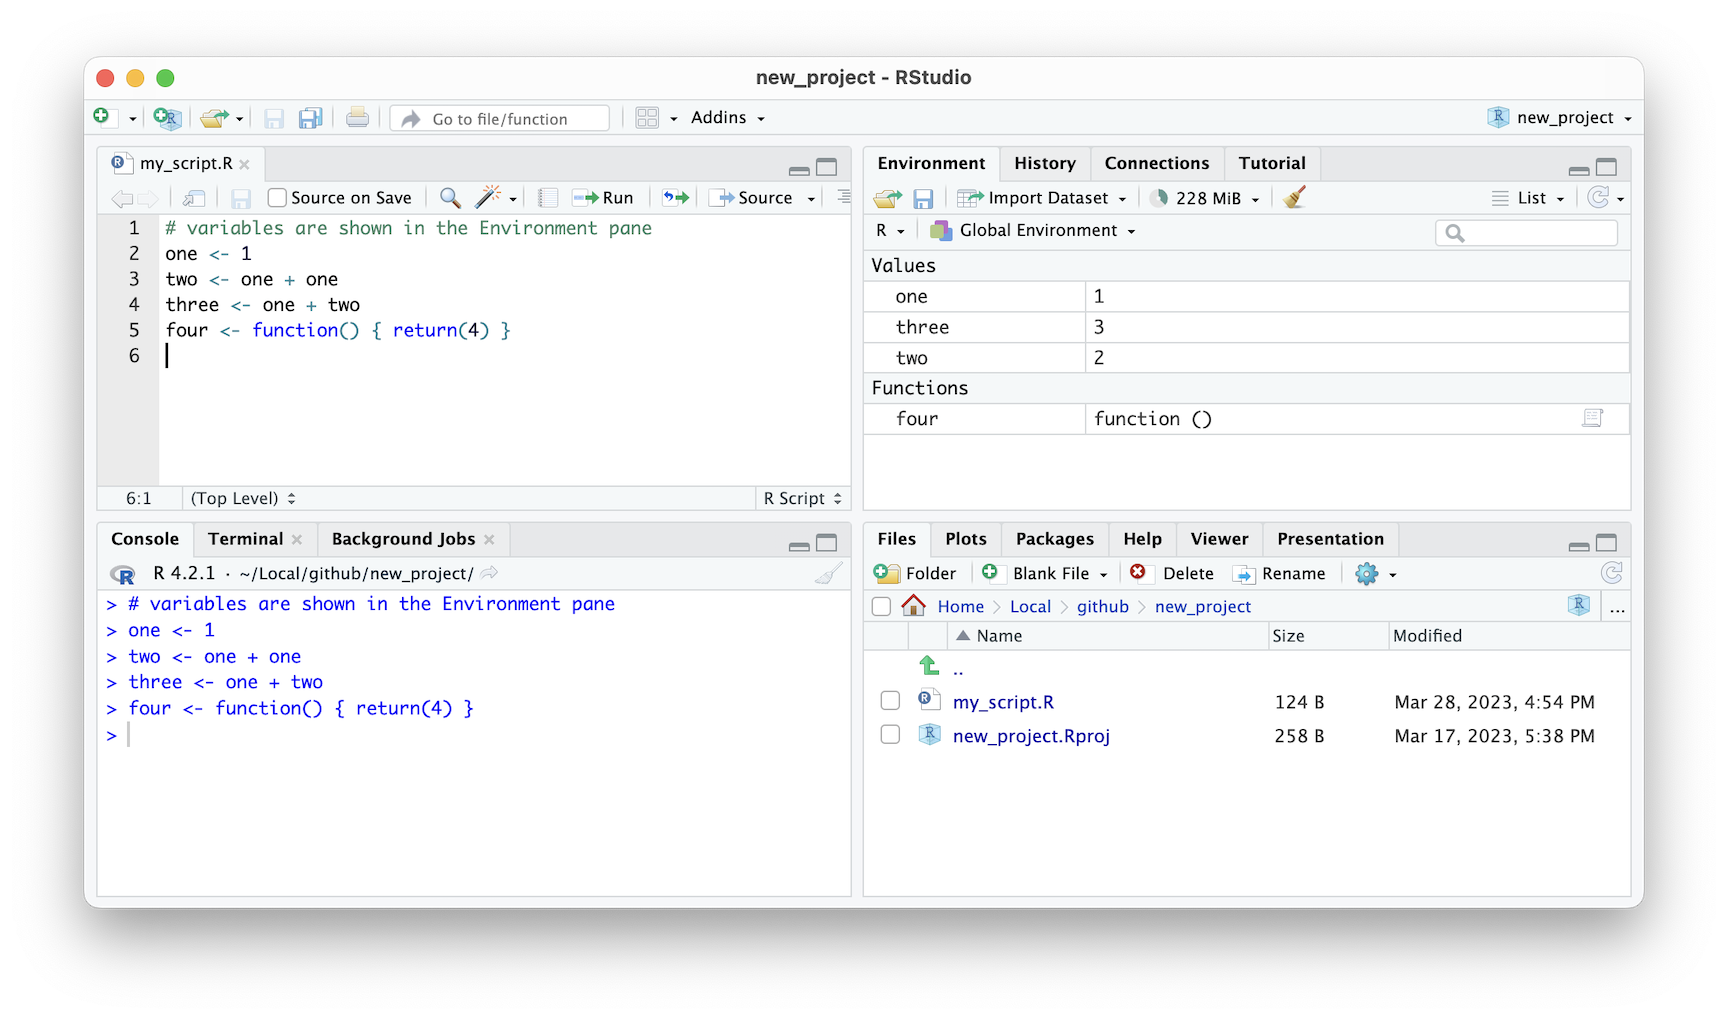
\includegraphics[width=31.94in]{images/02_025_environment} \caption{\label{fig:2025}RStudio IDE environment window}\label{fig:2025}
\end{figure}

\hypertarget{usage-..-running-lines-of-code-in-rstudio}{%
\subsection{Usage .. Running lines of code in RStudio}\label{usage-..-running-lines-of-code-in-rstudio}}

\hypertarget{run-from-the-editor-recommended}{%
\subsubsection{Run from the editor (recommended)}\label{run-from-the-editor-recommended}}

\begin{enumerate}
\def\labelenumi{\arabic{enumi}.}
\tightlist
\item
  Type in the code in the Editor (top-left pane)
\item
  Put editor cursor anywhere on that line
\item
  Press Ctrl/CMD+Enter.
\item
  Multiple lines: highlight multiple lines then press Ctrl/CMD+Enter \#\#\#\# Run from the onsole (occasionally)
\item
  Type code into Console (bottom-left) after the `\textgreater{}'
\item
  Press Enter.
\item
  Multiple lines, not advised, but copy and paste multiple lines into console then press Enter.
\end{enumerate}

\hypertarget{packages}{%
\section{Packages}\label{packages}}

\hypertarget{what-are-r-packages}{%
\subsection{What are R Packages?}\label{what-are-r-packages}}

R packages are a powerful tool in the R programming language that allow you to easily use code written by others in your own projects. They can save a lot of time and effort in the development of your own code, as they often provide new functions to deal with specific problems. For example, the popular ggplot2 package provides a variety of functions to help you create beautiful visualizations, while the mzR package allows you to read mass spectrometry data files with ease. Additionally, the twitteR package is a great tool for accessing Twitter data and conducting analysis.

\hypertarget{where-to-get-r-packages}{%
\subsection{Where to get R Packages}\label{where-to-get-r-packages}}

It's worth noting that packages can be written by anyone, which means that their quality can vary widely. While there are many high-quality packages available, it's important to be wary of randomly coming across packages on the internet. To ensure that you're working with trustworthy code, it's a good idea to stick with well-established and frequently updated packages from reputable sources such as the CRAN (The Comprehensive R Archive Network) and Bioconductor repositories. By doing so, you can ensure that your code is reliable, efficient, and secure.

\begin{itemize}
\tightlist
\item
  CRAN \href{https://cran.r-project.org/}{cran.r-project.org}
\item
  Bioconductor \href{https://bioconductor.org/}{bioconductor.org}
\item
  GitHub \href{https://github.com/}{github.com}
\end{itemize}

In addition to using established packages, it's also possible to create your own packages in R. This is a great way to share your own code with others and make it accessible to a wider audience. When creating a package, it's important to follow a set of best practices to ensure that your code is well-documented, easy to use, and compatible with other packages. This includes providing clear and concise documentation, including examples and tutorials, and following established coding conventions.

Another important consideration when working with R packages is version control. It's essential to keep track of the versions of the packages you're using, as updates can sometimes break existing code. By using a tool like Git or GitHub, you can easily manage different versions of your code and keep track of changes over time. This can be especially useful when collaborating with others on a project.

Overall, R packages are an essential tool for anyone working with R. By using established packages and following best practices when creating your own, you can ensure that your code is efficient, reliable, and easy to use. And by using version control, you can keep track of changes over time and collaborate effectively with others.

\hypertarget{installing-r-packages}{%
\subsection{Installing R Packages}\label{installing-r-packages}}

When working with R, it is important to understand how to install packages. R packages are collections of functions, data, and documentation that extend the capabilities of R. Most R packages have binary versions available for direct installation with no additional steps required. Binary packages are pre-compiled and ready-to-use packages that are platform-specific. They can be installed with the \texttt{install.packages()} function in R.

\hfill\break

\begin{longtable}[]{@{}
  >{\raggedright\arraybackslash}p{(\columnwidth - 2\tabcolsep) * \real{0.2083}}
  >{\raggedright\arraybackslash}p{(\columnwidth - 2\tabcolsep) * \real{0.7917}}@{}}
\toprule\noalign{}
\endhead
\bottomrule\noalign{}
\endlastfoot

\includegraphics[width=\textwidth,height=0.70833in]{images/01.png} & Follow the examples below to install all the required packages used in this book. Jump to the following section if you run into any issues. Use the copy-paste button in the top-right of each code block. \\
\end{longtable}

\hfill\break

\hypertarget{installing-from-cran}{%
\subsubsection*{Installing from CRAN}\label{installing-from-cran}}
\addcontentsline{toc}{subsubsection}{Installing from CRAN}

\begin{Shaded}
\begin{Highlighting}[]
\CommentTok{\# this installs all of the packages in the tidyverse collection}
\FunctionTok{install.packages}\NormalTok{(}\StringTok{\textquotesingle{}tidyverse\textquotesingle{}}\NormalTok{)}
\end{Highlighting}
\end{Shaded}

\hypertarget{installing-from-bioconductor}{%
\subsubsection*{Installing from Bioconductor}\label{installing-from-bioconductor}}
\addcontentsline{toc}{subsubsection}{Installing from Bioconductor}

\begin{Shaded}
\begin{Highlighting}[]
\CommentTok{\# do this once to install the Bioconductor Package Manager}
\FunctionTok{install.packages}\NormalTok{(}\StringTok{"BiocManager"}\NormalTok{)}
\CommentTok{\# this installs the mzR package}
\NormalTok{BiocManager}\SpecialCharTok{::}\FunctionTok{install}\NormalTok{(}\FunctionTok{c}\NormalTok{(}\StringTok{"mzR"}\NormalTok{, }\StringTok{"xcms"}\NormalTok{, }\StringTok{"MSstats"}\NormalTok{, }\StringTok{"MSnbase"}\NormalTok{))}
\end{Highlighting}
\end{Shaded}

\hypertarget{installing-from-github}{%
\subsubsection*{Installing from GitHub}\label{installing-from-github}}
\addcontentsline{toc}{subsubsection}{Installing from GitHub}

\begin{Shaded}
\begin{Highlighting}[]
\CommentTok{\# do this once to install the devtools package }
\FunctionTok{install.packages}\NormalTok{(}\StringTok{"devtools"}\NormalTok{)}
\CommentTok{\# this installs the tidyproteomics package}
\FunctionTok{install\_github}\NormalTok{(}\StringTok{"jeffsocal/tidyproteomics"}\NormalTok{)}
\end{Highlighting}
\end{Shaded}

\hfill\break

\begin{longtable}[]{@{}
  >{\raggedright\arraybackslash}p{(\columnwidth - 2\tabcolsep) * \real{0.1164}}
  >{\raggedright\arraybackslash}p{(\columnwidth - 2\tabcolsep) * \real{0.8836}}@{}}
\toprule\noalign{}
\endhead
\bottomrule\noalign{}
\endlastfoot

\includegraphics[width=\textwidth,height=0.70833in]{images/01.png} & There maybe several additional packages to install including additional operating system level installs. Go to the \href{https://jeffsocal.github.io/tidyproteomics/}{tidyproteomics} webpage for additional installation help. \textbar{} \\
\end{longtable}

\hfill\break

\hypertarget{potential-gotchas}{%
\subsection{Potential Gotchas}\label{potential-gotchas}}

However, there are cases where a binary version of a package may not be available. This could be because the package is new or has just been updated. In such cases, the package may need to be compiled before it can be installed. Compiling a package involves converting the source code into machine-readable code that can be executed.

To compile R packages, you'll need to have the necessary programs and libraries installed on your computer. For Windows, you'll need to install RTools, which provides the necessary tools for package compilation. For Mac, you'll need to install Command Line Tools. Once these tools are installed, you can use them to compile packages that are not available as binaries.

However, it's worth noting that package compilation can sometimes fail for various reasons. This can be frustrating, especially if you're new to R. Therefore, it is generally recommended to stick with using binary packages whenever possible. Binary packages are more stable and easier to install, making them the preferred option for most users.

In summary, when working with R, it's important to understand how to install packages. Most packages have binary versions available for direct installation, but there may be cases where you need to compile a package yourself. While package compilation can be useful in some cases, it can also be frustrating and time-consuming. Therefore, it's generally recommended to stick with using binary packages whenever possible.

\hypertarget{packages-utilized-in-this-book}{%
\section{Packages Utilized in This Book}\label{packages-utilized-in-this-book}}

\hypertarget{tidyverse}{%
\subsection*{tidyverse}\label{tidyverse}}
\addcontentsline{toc}{subsection}{tidyverse}

The Tidyverse R package is a collection of data manipulation and visualization packages for the R programming language. It includes popular packages such as dplyr, ggplot2, and tidyr, among others. The Tidyverse R package is a powerful and versatile tool for data analysis in R. It includes a collection of data manipulation and visualization packages designed to work seamlessly together, making it easy to analyze and visualize data in R.

\begin{Shaded}
\begin{Highlighting}[]
\FunctionTok{library}\NormalTok{(tidyverse)}
\end{Highlighting}
\end{Shaded}

The \textbf{readr} package provides a versatile means of reading data from various formats, such as comma-separated (CSV) and tab-separated (TSV) delimitated flat files. In addition to its versatility, the \textbf{readr} package is also known for its speed and efficiency. It is designed to be faster than the base R functions for reading in data, making it an ideal choice for working with large datasets.

\begin{Shaded}
\begin{Highlighting}[]
\NormalTok{tbl }\OtherTok{\textless{}{-}} \StringTok{"./data/table\_peptide\_fragmnets.csv"} \SpecialCharTok{\%\textgreater{}\%} \FunctionTok{read\_csv}\NormalTok{()}
\end{Highlighting}
\end{Shaded}

\begin{verbatim}
## Rows: 14 Columns: 7
## -- Column specification ---------------------------------------------------------------------------
## Delimiter: ","
## chr (4): ion, seq, pair, type
## dbl (3): mz, z, pos
## 
## i Use `spec()` to retrieve the full column specification for this data.
## i Specify the column types or set `show_col_types = FALSE` to quiet this message.
\end{verbatim}

The \textbf{tibble} package embodies a modern, flexible take on the data table, making it a powerful tool for data analysis in R. This package includes a suite of functions that allow you to easily manipulate and reshape data. It also has a printing method that makes it easy to view and explore data, even when dealing with large datasets. Additionally, tibble objects are designed to work seamlessly with other Tidyverse packages, such as \textbf{dplyr} and \textbf{tidyr}, making it easy to switch between packages and maintain a consistent syntax.

\begin{Shaded}
\begin{Highlighting}[]
\FunctionTok{print}\NormalTok{(tbl)}
\end{Highlighting}
\end{Shaded}

\begin{verbatim}
## # A tibble: 14 x 7
##    ion      mz     z seq     pair    pos type     
##    <chr> <dbl> <dbl> <chr>   <chr> <dbl> <chr>    
##  1 b1+    98.1     1 P       p01       1 b        
##  2 y1+   148.      1 E       p06       1 y        
##  3 b2+   227.      1 PE      p02       2 b        
##  4 y2+   263.      1 DE      p05       2 y        
##  5 b3+   324.      1 PEP     p03       3 b        
##  6 y3+   376.      1 IDE     p04       3 y        
##  7 MH++  401.      2 PEPTIDE p00      NA precursor
##  8 b4+   425.      1 PEPT    p04       4 b        
##  9 y4+   477.      1 TIDE    p03       4 y        
## 10 b5+   538.      1 PEPTI   p05       5 b        
## 11 y5+   574.      1 PTIDE   p02       5 y        
## 12 b6+   653.      1 PEPTID  p06       6 b        
## 13 y6+   703.      1 EPTIDE  p01       6 y        
## 14 MH+   800.      1 PEPTIDE p00      NA precursor
\end{verbatim}

The \textbf{readxl} package is a complement to \textbf{readr} providing a means to read Excel files, both legacy .xls and the current xml-based .xlsx. It is capable of reading many different types of data, including dates, times, and various numeric formats. The package also provides options for specifying sheet names, selecting specific columns and rows, and handling missing values.

The \textbf{dplyr} package is widely known and used among data scientists and analysts for its interface that allows for easy and efficient data manipulation in \emph{tibbles}. Providing a set of ``verbs'' that are designed to solve common tasks in data transformations and summaries, such as filtering, arranging, and summarizing data, all designed to work seamlessly with other Tidyverse packages making it easy to switch between packages and maintain a consistent syntax. One of the key benefits of the \textbf{dplyr} package is its ease of use, making it perfect for beginners and advanced users alike. It is widely used in the R community and is a valuable tool for anyone working with R and data tables.

\begin{Shaded}
\begin{Highlighting}[]
\NormalTok{tbl }\SpecialCharTok{\%\textgreater{}\%} 
  \FunctionTok{filter}\NormalTok{(type }\SpecialCharTok{!=} \StringTok{\textquotesingle{}precursor\textquotesingle{}}\NormalTok{) }\SpecialCharTok{\%\textgreater{}\%} 
  \FunctionTok{group\_by}\NormalTok{(type) }\SpecialCharTok{\%\textgreater{}\%}
  \FunctionTok{summarise}\NormalTok{(}
    \AttributeTok{num\_ions =} \FunctionTok{n}\NormalTok{(),}
    \AttributeTok{avg\_mass =} \FunctionTok{mean}\NormalTok{(mz)}
\NormalTok{  )}
\end{Highlighting}
\end{Shaded}

\begin{verbatim}
## # A tibble: 2 x 3
##   type  num_ions avg_mass
##   <chr>    <int>    <dbl>
## 1 b            6     378.
## 2 y            6     424.
\end{verbatim}

The \textbf{tidyr} package contains a set of data table transformations, including pivotting rows to columns, splitting a single column into multiple ones, and tidying or cleaning up data tables for a more usable structure. These transformations are essential for dealing with real-world data tables, which are often messy and irregular. By using \textbf{tidyr}, you can quickly and easily manipulate data tables to extract the information you need and prepare them for further analysis.

\begin{Shaded}
\begin{Highlighting}[]
\NormalTok{tbl }\SpecialCharTok{\%\textgreater{}\%} 
  \FunctionTok{filter}\NormalTok{(type }\SpecialCharTok{==} \StringTok{\textquotesingle{}precursor\textquotesingle{}}\NormalTok{) }\SpecialCharTok{\%\textgreater{}\%} 
  \FunctionTok{pivot\_wider}\NormalTok{(z, }\AttributeTok{names\_from =} \StringTok{\textquotesingle{}type\textquotesingle{}}\NormalTok{, }\AttributeTok{values\_from =} \StringTok{\textquotesingle{}mz\textquotesingle{}}\NormalTok{)}
\end{Highlighting}
\end{Shaded}

\begin{verbatim}
## # A tibble: 2 x 2
##       z precursor
##   <dbl>     <dbl>
## 1     2      401.
## 2     1      800.
\end{verbatim}

The \textbf{ggplot2} package stands out as the most advanced and comprehensive package for transforming tabulated data into meaningful and informative graphics. With its wide range of visualization tools, this package allows you to create expressive and compelling graphics that not only look great but also convey detailed information in a clear and concise manner. Apart from other visualization tools, \textbf{ggplot2} takes a layered approach to creating graphics, allowing for the additive layering of additional data, labels, legends, and annotations, which helps to provide a more comprehensive view of your analysis.

\begin{Shaded}
\begin{Highlighting}[]
\NormalTok{tbl }\SpecialCharTok{\%\textgreater{}\%}
  \FunctionTok{mutate}\NormalTok{(}\AttributeTok{int =} \FunctionTok{rnorm}\NormalTok{(}\FunctionTok{n}\NormalTok{(), }\AttributeTok{mean =} \FloatTok{1e5}\NormalTok{, }\AttributeTok{sd=}\FloatTok{5e4}\NormalTok{),}
         \AttributeTok{relative\_int =}\NormalTok{ int}\SpecialCharTok{/}\FunctionTok{max}\NormalTok{(int) }\SpecialCharTok{*} \DecValTok{100}\NormalTok{) }\SpecialCharTok{\%\textgreater{}\%}
  \FunctionTok{ggplot}\NormalTok{(}\FunctionTok{aes}\NormalTok{(mz, relative\_int, }\AttributeTok{color=}\NormalTok{type)) }\SpecialCharTok{+}
  \FunctionTok{geom\_segment}\NormalTok{(}\FunctionTok{aes}\NormalTok{(}\AttributeTok{xend =}\NormalTok{ mz, }\AttributeTok{yend =} \DecValTok{0}\NormalTok{)) }\SpecialCharTok{+}
  \FunctionTok{labs}\NormalTok{(}\AttributeTok{title =} \StringTok{"Simulated MS/MS Spectrum"}\NormalTok{)}
\end{Highlighting}
\end{Shaded}

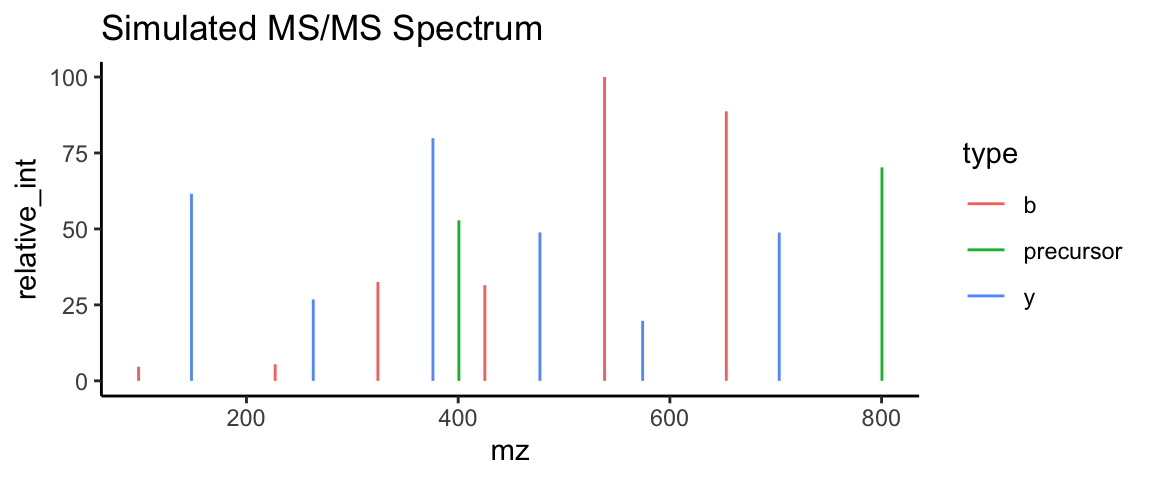
\includegraphics{_main_files/figure-latex/unnamed-chunk-9-1.pdf}

One of the key benefits of using the Tidyverse is the standardization of syntax and functions across each package. This means that once you learn the basics of one package, you can easily switch to another package and be confident in your ability to use it. This makes it easier to create reproducible code and improves the efficiency of your data analysis.

The Tidyverse is widely used in the R community and is a valuable tool for any data scientist or analyst working with R. It is especially useful for those who need to manipulate and visualize data quickly and efficiently, without sacrificing accuracy. Whether you are new to R or an experienced user, the Tidyverse is a must-have tool in your data analysis toolkit.

\hypertarget{mass-spectrometry-specific-packages}{%
\subsection*{Mass Spectrometry Specific Packages}\label{mass-spectrometry-specific-packages}}
\addcontentsline{toc}{subsection}{Mass Spectrometry Specific Packages}

This book, while providing a beginners level guide to R programming, also introduces several mass spectrometry-specific packages in many of the code examples. While these examples may only touch on some of their functions, the last chapter is dedicated to a more formal, albeit not comprehensive introduction to many of these packages. For example the \texttt{mzR} package, which enables users to read and process mass spectrometry data, as well as the \texttt{xcms} package, which is used for preprocessing and feature detection. Additionally, the book introduces the \texttt{MSnbase} package, which provides a framework for quantitative and qualitative analysis of mass spectrometry data, and the \texttt{MSstats} package, which is used for statistical analysis of quantitative proteomics experiments. Lastly, the book covers the \texttt{tidyproteomics} package, which provides a collection of tools for analyzing post-analysis quantitative proteomics data using a framework similar to the \texttt{tidyverse}.

\hypertarget{r-studio-projects}{%
\chapter{R Studio Projects}\label{r-studio-projects}}

Project are how RStudio organizes your work. Think of project as singular goal oriented collection. There are no rules but some basic organizational tips should help simplify your project.

\hypertarget{creating}{%
\section{Creating}\label{creating}}

Creating a new project is very forgiving, you can create a new directory with a project name, or create a project out of an existing directory.

Either 1. Click on the drop down in the top right 2. OR: Under the menu item select \texttt{File\ \textgreater{}\ New\ Project}

In the \texttt{New\ Project\ Wizard} select \texttt{New\ Directory\ \textgreater{}\ New\ Project}, enter the name of the project and click \texttt{Create\ Project}.

\begin{figure}
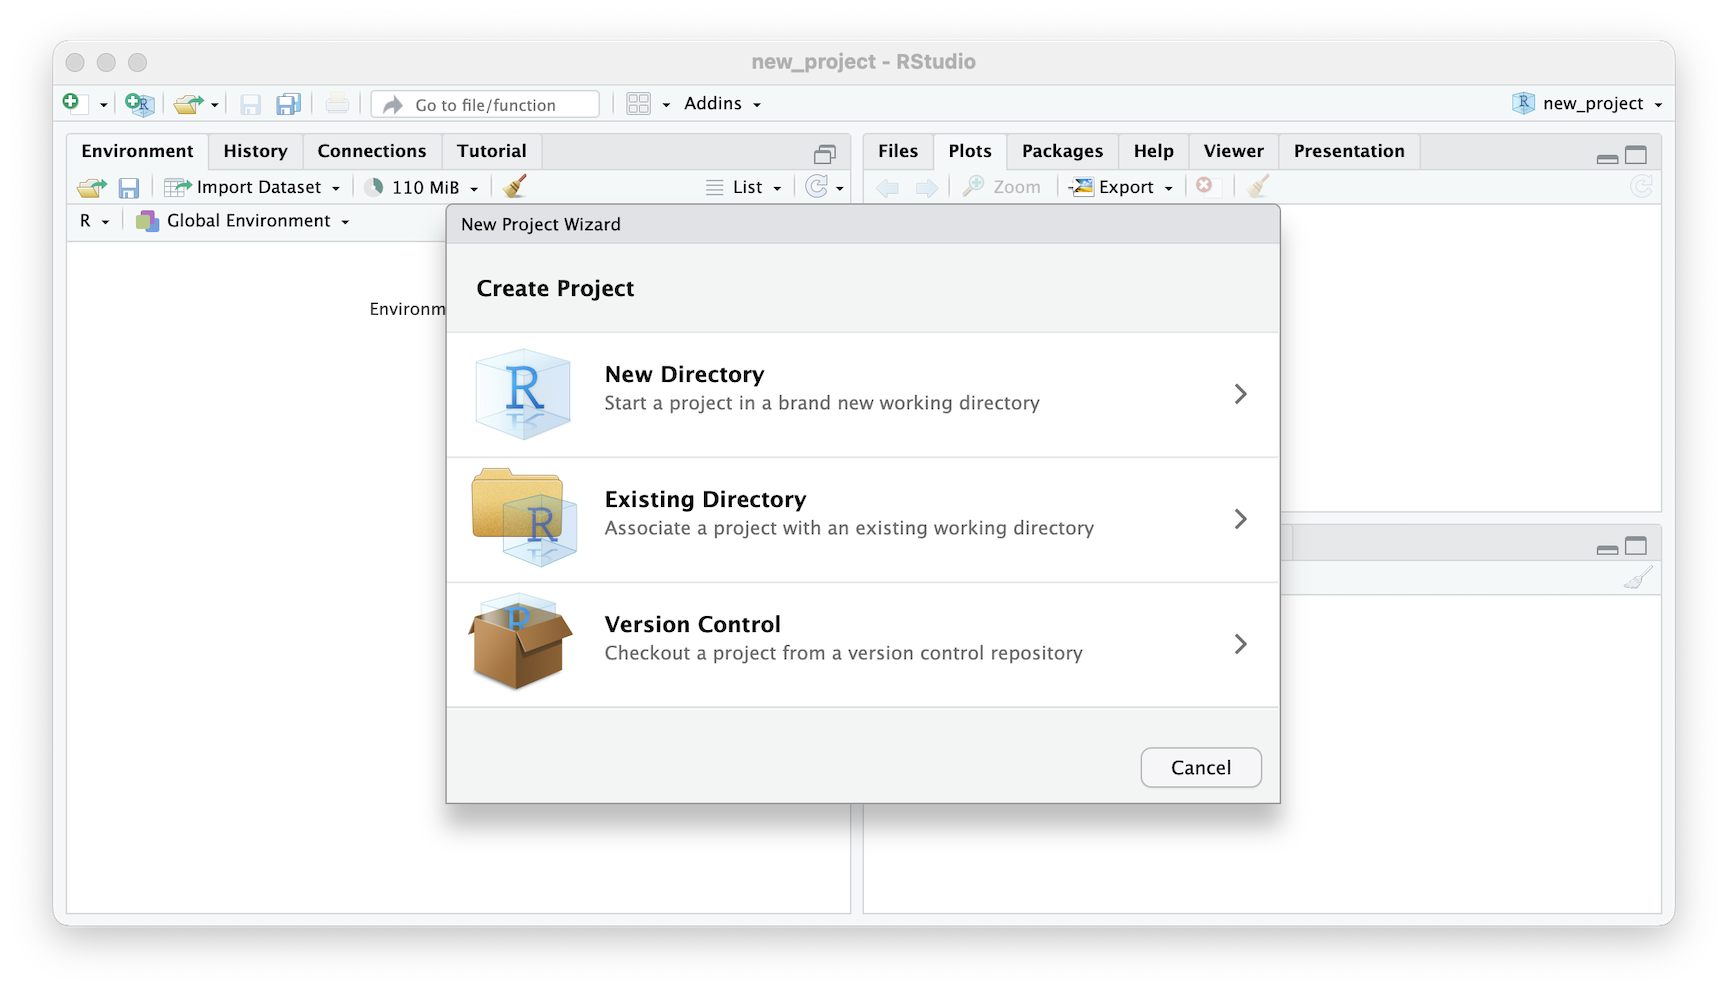
\includegraphics[width=30.72in]{images/03_021_new_project_01} \caption{\label{fig:3201}RStudio Create New Project}\label{fig:3201}
\end{figure}
\begin{figure}
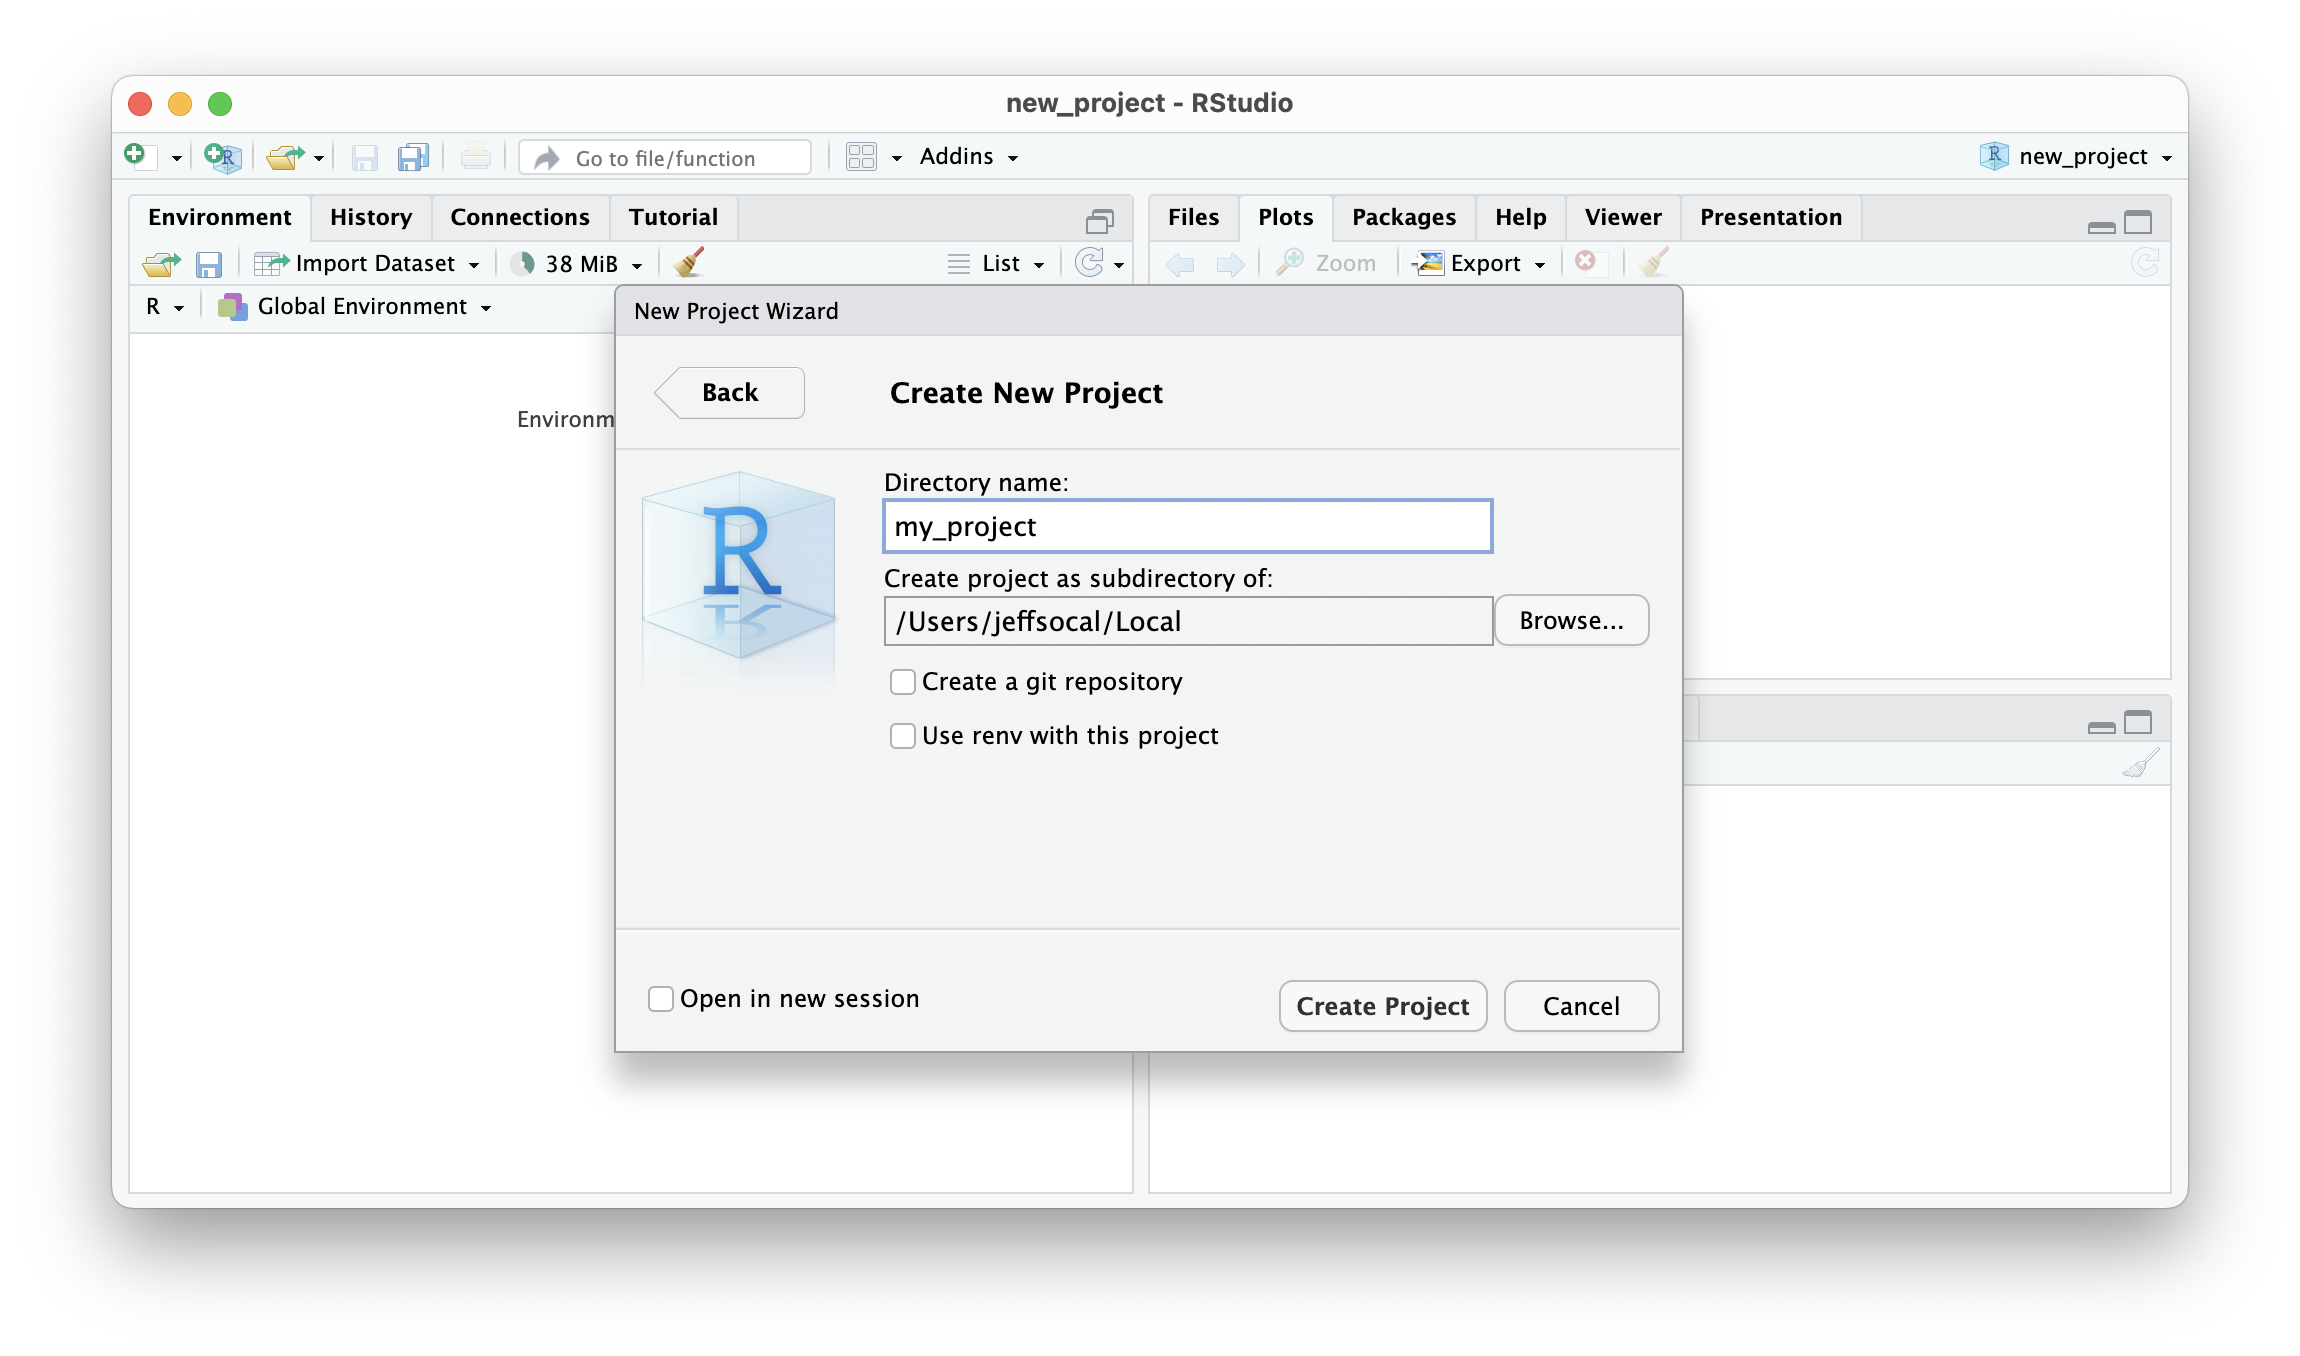
\includegraphics[width=31.94in]{images/03_021_new_project_02} \caption{\label{fig:3202}RStudio Create New Project}\label{fig:3202}
\end{figure}

\hypertarget{editing}{%
\section{Editing}\label{editing}}

\hypertarget{organizing}{%
\section{Organizing}\label{organizing}}

\hypertarget{data}{%
\subsection{Data}\label{data}}

\hypertarget{scripts}{%
\subsection{Scripts}\label{scripts}}

\hypertarget{results}{%
\subsection{Results}\label{results}}

\hypertarget{tables}{%
\subsubsection{Tables}\label{tables}}

\hypertarget{plots}{%
\subsubsection{Plots}\label{plots}}

\hypertarget{exercises}{%
\section*{Exercises}\label{exercises}}
\addcontentsline{toc}{section}{Exercises}

\begin{longtable}[]{@{}
  >{\raggedright\arraybackslash}p{(\columnwidth - 2\tabcolsep) * \real{0.2764}}
  >{\raggedright\arraybackslash}p{(\columnwidth - 2\tabcolsep) * \real{0.7236}}@{}}
\toprule\noalign{}
\endhead
\bottomrule\noalign{}
\endlastfoot

\includegraphics[width=\textwidth,height=0.70833in]{images/07.png} & \begin{minipage}[t]{\linewidth}\raggedright
\begin{itemize}
\item
  Create a new R Studio Project and name it \textbf{001\_new\_project}.
\item
  Create a new R script, add your name and date at the top as comments.
\item
  Create an R script file, write something (anything), and save it as \textbf{01\_test}.
\item
  Create a new R script, add your name and date at the top as comments.
\item
  Locate your new project on your PC.
\end{itemize}
\end{minipage} \\
\end{longtable}

\hypertarget{r-syntax}{%
\chapter{R Syntax}\label{r-syntax}}

Welcome to the R Book! In this chapter, we will explore the basics of R, a powerful programming language used for statistical computing and graphics.

At its most fundamental level, R is a calculator capable of performing simple, and complex, mathematical operations. It can read and write data to and from files, manipulate the data, calculate summaries and plot visual representations of the data. Essentially, it is a programmatic version of a spreadsheet program.

However, R is much more than just a calculator. It is also a platform for conducting complex analyses, statistical evaluations, predictive inferencing, and machine learning. With R, you can explore and visualize data in a variety of ways, perform advanced statistical analyses, and build predictive models.

In this chapter, we will start by examining the simplest operations of R. We will cover basic arithmetic, working with variables, and creating basic plots. By the end of this chapter, you will have a solid understanding of the fundamentals of R and be ready to tackle more complex topics.

So, let's get started!

\hfill\break

\begin{longtable}[]{@{}
  >{\raggedright\arraybackslash}p{(\columnwidth - 2\tabcolsep) * \real{0.3434}}
  >{\raggedright\arraybackslash}p{(\columnwidth - 2\tabcolsep) * \real{0.6566}}@{}}
\toprule\noalign{}
\endhead
\bottomrule\noalign{}
\endlastfoot
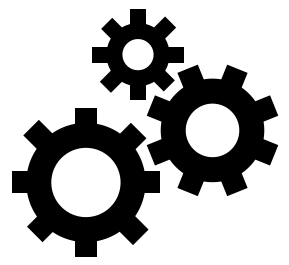
\includegraphics[width=\textwidth,height=0.70833in]{images/03.png} & \begin{minipage}[t]{\linewidth}\raggedright
\textbf{At the end of this chapter you should be able to}

\begin{itemize}
\item
  Understand R's syntax, variables, operators and functions.
\item
  Create and edit a project in RStudio.
\end{itemize}
\end{minipage} \\
\end{longtable}

\hfill\break

\hypertarget{reserved-words}{%
\section{Reserved Words}\label{reserved-words}}

As we begin our journey, it's important to keep in mind that there are certain reserved words that carry a special meaning and cannot be used as identifiers. These words have been set aside by the R programming language, and using them as variable names or function names could lead to errors in your code.

Therefore, before we dive too deeply into our R programming endeavors, let's take a moment to familiarize ourselves with these reserved words. This will help us avoid potential issues down the road and ensure that our code runs smoothly.

\begin{Shaded}
\begin{Highlighting}[]
\CommentTok{\# to read more about them type}
\NormalTok{?reserved}
\end{Highlighting}
\end{Shaded}

\begin{longtable}[]{@{}
  >{\raggedright\arraybackslash}p{(\columnwidth - 2\tabcolsep) * \real{0.4167}}
  >{\raggedright\arraybackslash}p{(\columnwidth - 2\tabcolsep) * \real{0.5833}}@{}}
\toprule\noalign{}
\begin{minipage}[b]{\linewidth}\raggedright
Word
\end{minipage} & \begin{minipage}[b]{\linewidth}\raggedright
Use
\end{minipage} \\
\midrule\noalign{}
\endhead
\bottomrule\noalign{}
\endlastfoot
\texttt{if}, \texttt{else} & flow control, part of the if-then-else statement \\
\texttt{for}, \texttt{repeat}, \texttt{while}, \texttt{break}, \texttt{next} & flow control, part of the for-loop statement \\
\texttt{function} & basis for defining new algorithms \\
\texttt{TRUE}, \texttt{FALSE} & Boolean logic values \\
\texttt{NULL} & an undefined value \\
\texttt{Inf} , \texttt{-Inf} & an infinite value (eg. \texttt{1/0} ) \\
\texttt{NaN} & `not a number' \\
\texttt{NA} & a missing value indicator \\
\end{longtable}

\hfill\break

\begin{longtable}[]{@{}
  >{\raggedright\arraybackslash}p{(\columnwidth - 2\tabcolsep) * \real{0.1635}}
  >{\raggedright\arraybackslash}p{(\columnwidth - 2\tabcolsep) * \real{0.8365}}@{}}
\toprule\noalign{}
\endhead
\bottomrule\noalign{}
\endlastfoot

\includegraphics[width=\textwidth,height=0.70833in]{images/01.png} & A \texttt{Null} results when a value is missing and could be a \emph{string} or a \emph{numeric}, where as a NA results when a known value, such as in a column of numbers, is missing. \textbar{} \\
\end{longtable}

\hfill\break

\hypertarget{syntax}{%
\section{Syntax}\label{syntax}}

Welcome to the R Book! Whether you're just starting out or a seasoned pro, understanding the different components of R code is essential for writing high-quality, efficient R programs. In this section, we'll take a deep dive into the various components of R code that you should be familiar with.

R input is composed of typed characters that represent different parts of a process or mathematical operation. These characters come together to form what we call R code. It's important to note that R code is not just a random collection of characters - each character serves a specific purpose and contributes to the larger structure of the code. As such, understanding the different components of R code is key to writing effective and efficient R programs.

So, what are these different components of R code? Below, we've provided some examples to help you get started:

\begin{longtable}[]{@{}
  >{\raggedright\arraybackslash}p{(\columnwidth - 2\tabcolsep) * \real{0.3780}}
  >{\raggedright\arraybackslash}p{(\columnwidth - 2\tabcolsep) * \real{0.6220}}@{}}
\toprule\noalign{}
\endhead
\bottomrule\noalign{}
\endlastfoot
\ref{comments} comments & \texttt{\#\ this\ is\ an\ important\ note} \\
\ref{strings} strings & \texttt{"letters"} or \texttt{"numbers"} in quotes \\
\ref{numbers} numbers & \texttt{1} integers or \texttt{1.000002} floats \\
\ref{operators} operators & \texttt{+}, \texttt{-}, \texttt{/}, \texttt{*}, \ldots{} \\
\ref{variables} variables & \texttt{var\ \textless{}-\ 2} containers for information \\
\ref{statements} statements & \texttt{==} exactly the same, \texttt{!=} not the same \\
\ref{functions} functions & \texttt{add(x,\ y)} complex code in a convenient wrapper \\
\end{longtable}

By understanding these different components of R code, you'll be well on your way to writing effective and efficient R programs. So let's dive in and get started!

\begin{Shaded}
\begin{Highlighting}[]
\CommentTok{\# adding two numbers here and storing it as a variable}
\NormalTok{four }\OtherTok{\textless{}{-}} \DecValTok{2} \SpecialCharTok{+} \DecValTok{2}

\CommentTok{\# using the function \textquotesingle{}cat\textquotesingle{} to print out my variable along with some text}
\FunctionTok{cat}\NormalTok{(}\StringTok{"my number is "}\NormalTok{, four)}
\end{Highlighting}
\end{Shaded}

\begin{verbatim}
## my number is  4
\end{verbatim}

\hfill\break

\begin{longtable}[]{@{}
  >{\raggedright\arraybackslash}p{(\columnwidth - 2\tabcolsep) * \real{0.3119}}
  >{\raggedright\arraybackslash}p{(\columnwidth - 2\tabcolsep) * \real{0.6881}}@{}}
\toprule\noalign{}
\endhead
\bottomrule\noalign{}
\endlastfoot

\includegraphics[width=\textwidth,height=0.70833in]{images/01.png} & R does not have an line ending character such as \texttt{;} in java, PHP or C++ \\
\end{longtable}

\hfill\break

\hypertarget{comments}{%
\subsection{Comments}\label{comments}}

Comments are essential parts of the code you will write. They help explain why you are taking a certain approach to the problem, either for you to remember at a later time or for a colleague. Comments in other coding languages, including R package development, can become quite expressive, representing parts and structures to a larger documentation effort. Here, however, comments are just simple text that gets ignored by the R interpreter. You can put anything you want in comments.

\begin{Shaded}
\begin{Highlighting}[]
\NormalTok{oops, not a comment}
\end{Highlighting}
\end{Shaded}

\begin{Shaded}
\begin{Highlighting}[]
\CommentTok{\# This is a comment}

\CommentTok{\# and here a comment tag is used to ignore legitimate R code}
\CommentTok{\# four \textless{}{-} 2 + 2 }
\NormalTok{four }\OtherTok{\textless{}{-}} \DecValTok{2} \SpecialCharTok{*} \DecValTok{2}
\end{Highlighting}
\end{Shaded}

\hypertarget{strings}{%
\subsection{Strings}\label{strings}}

Strings are essentially a sequence of characters, consisting of letters or numbers. They are commonly used in programming languages and are used to represent text-based data. A string can be as simple as a single character, such as ``A'', or it can be a longer sequence of characters such as ``Hello, World!''. Strings are often used to store data that requires text manipulation, such as usernames, passwords, and email addresses. In contrast to words, which are made up of a specific combination of letters to represent a linguistic term, strings do not follow any specific rules of composition and can be a random or semi-random sequence of characters.

\begin{Shaded}
\begin{Highlighting}[]
\CommentTok{\# a string can be a word, this is a string variable}
\NormalTok{three }\OtherTok{\textless{}{-}} \DecValTok{1} \SpecialCharTok{+} \DecValTok{2}
\CommentTok{\# or an abbreviation, this is a variable (thr) representing the string "three"}
\NormalTok{thr }\OtherTok{\textless{}{-}} \StringTok{"three"} 
\CommentTok{\# a mass spec reference}
\NormalTok{peptide }\OtherTok{\textless{}{-}} \StringTok{"QWERTK"}
\CommentTok{\# or an abbreviated variable}
\NormalTok{pep }\OtherTok{\textless{}{-}} \StringTok{"QWERTK"}
\end{Highlighting}
\end{Shaded}

When working with R programming language, it is essential to note that strings play a crucial role in the syntax used. Strings, which define text characters, are used to represent data in R, and they must be enclosed in quotes. Failure to do so will result in the interpreter assuming that you are referring to a variable that is not enclosed in quotes.

For instance, in the example above, the \texttt{peptide} variable contains the string of letters representing the peptide amino acid sequence \texttt{"QWERTK"}. However, it is essential to note that there are no strict rules for how strings and variables are composed, except that variables \textbf{cannot} start with a number.

\begin{Shaded}
\begin{Highlighting}[]
\CommentTok{\# permitted}
\NormalTok{b4 }\OtherTok{\textless{}{-}} \DecValTok{1} \SpecialCharTok{+} \DecValTok{3}
\CommentTok{\# not permitted}
\NormalTok{4b }\OtherTok{\textless{}{-}} \DecValTok{1} \SpecialCharTok{+} \FloatTok{3.} \DocumentationTok{\#\# Error: unexpected symbol in "4b"}
\end{Highlighting}
\end{Shaded}

There are however, conventions that you can follow when constructing variable names that aid in the readability of the code and convey information about the contents. This is especially useful in long code blocks, or, when the code becomes more complex and divested across several files. For example:

\begin{Shaded}
\begin{Highlighting}[]
\CommentTok{\# a string containing a peptide sequence}
\NormalTok{str\_pep }\OtherTok{\textless{}{-}} \StringTok{"QWERTK"}

\CommentTok{\# a data table of m/z values and their identifications}
\NormalTok{tbl\_mz\_ids }\OtherTok{\textless{}{-}} \FunctionTok{read\_csv}\NormalTok{(}\StringTok{"somefile.csv"}\NormalTok{)}
\end{Highlighting}
\end{Shaded}

To learn more about and follow specific conventions, explore the following resources:

\begin{itemize}
\item
  \href{http://adv-r.had.co.nz/Style.html}{Hadley Wickham's Style Guide}
\item
  \href{https://google.github.io/styleguide/Rguide.html}{Google's style Guide}
\item
  \href{https://style.tidyverse.org/}{The tidyverse style guide}
\end{itemize}

\hypertarget{numbers}{%
\subsection{Numbers}\label{numbers}}

Numbers are the foundation upon which all data analysis is built. Without numbers, we would not be able to perform calculations, identify patterns, or draw conclusions from our data. In the programming language R, there are two main types of numbers: \texttt{integers} and \texttt{floats}. An integer is a whole number with no decimal places, while a float is a number with decimal places. Understanding the difference between these two types of numbers is essential for accurate numerical analysis.

In R, integers are represented as whole numbers, such as 1, 2, 3, and so on, while floats are represented with a decimal point, such as 1.5, 2.75, and so on. It is important to note that integers occupy less space in memory than floats, which can be a consideration when working with large datasets. This means that when possible, it is generally better to use integers over floats in R, as they are more efficient and can improve the overall performance of your code.

\begin{Shaded}
\begin{Highlighting}[]
\CommentTok{\# integers}
\DecValTok{1}\NormalTok{,  }\DecValTok{12345}\NormalTok{, }\SpecialCharTok{{-}}\DecValTok{17}\NormalTok{, }\DecValTok{0}
\end{Highlighting}
\end{Shaded}

Numbers are the foundation upon which all data analysis is built. Without numbers, we would not be able to perform calculations, identify patterns, or draw conclusions from our data. In the programming language R, there are two main types of numbers: \texttt{integers} and \texttt{floats}.

An integer is a whole number with no decimal places, while a float is a number with decimal places. In most programming languages, including R, integers are represented as whole numbers, such as 1, 2, 3, and so on, while floats are represented with a decimal point, such as 1.5, 2.75, and so on.

It is essential to understand the difference between these two types of numbers for accurate numerical analysis. While integers can only represent whole numbers, floats can represent fractions and decimals. Thus, if you need to represent a number that is not a whole number, you should use a float.

Moreover, it is important to note that integers occupy less space in memory than floats. This can be a consideration when working with large datasets, especially when the whole number is enough to represent the data. Therefore, when possible, it is generally better to use integers over floats in R, as they are more efficient and can improve the overall performance of your code.

\begin{Shaded}
\begin{Highlighting}[]
\CommentTok{\# floats}
\NormalTok{significand }\OtherTok{\textless{}{-}} \DecValTok{12345}
\NormalTok{exponent }\OtherTok{\textless{}{-}} \SpecialCharTok{{-}}\DecValTok{3}
\NormalTok{base }\OtherTok{\textless{}{-}} \DecValTok{10}

\CommentTok{\# 12.345 = 12345 * 10\^{}{-}3}
\NormalTok{significand }\SpecialCharTok{*}\NormalTok{ base }\SpecialCharTok{\^{}}\NormalTok{ exponent}
\end{Highlighting}
\end{Shaded}

\hypertarget{operators}{%
\subsection{Operators}\label{operators}}

Operators are fundamental components of programming that enable us to manipulate and process various data types. They are symbols that perform a specific action on one or more operands, which could be numeric values, variables, or even strings. Most commonly these symbols allow us to perform basic arithmetic operations such as addition, subtraction, multiplication, and division on numeric values, as well as more complex mathematical operations like exponentiation and modulus.

In addition to numeric values, operators can also manipulate string variables. For instance, we can use concatenation operators to join two or more strings together, which is particularly useful when working with text data. By utilizing operators, we can perform powerful operations that allow us to build complex programs and applications that can handle large amounts of data. Operators play a crucial role in programming, as they allow us to manipulate data in a way that would be difficult or impossible to achieve otherwise.

At their very basic, operators allow you to perform \textbf{calculations} ..

\begin{Shaded}
\begin{Highlighting}[]
\DecValTok{1} \SpecialCharTok{+} \DecValTok{2}
\end{Highlighting}
\end{Shaded}

\begin{verbatim}
## [1] 3
\end{verbatim}

\begin{Shaded}
\begin{Highlighting}[]
\DecValTok{1} \SpecialCharTok{/} \DecValTok{2}
\end{Highlighting}
\end{Shaded}

\begin{verbatim}
## [1] 0.5
\end{verbatim}

.. \textbf{assign} values to string variables ..

\begin{Shaded}
\begin{Highlighting}[]
\NormalTok{myvar }\OtherTok{\textless{}{-}} \DecValTok{1}
\end{Highlighting}
\end{Shaded}

.. and \textbf{compare} values.

\begin{Shaded}
\begin{Highlighting}[]
\DecValTok{1} \SpecialCharTok{==}\NormalTok{ myvar}
\end{Highlighting}
\end{Shaded}

\begin{verbatim}
## [1] TRUE
\end{verbatim}

\begin{Shaded}
\begin{Highlighting}[]
\DecValTok{2} \SpecialCharTok{!=}\NormalTok{ myvar }\SpecialCharTok{+}\NormalTok{ myvar}
\end{Highlighting}
\end{Shaded}

\begin{verbatim}
## [1] FALSE
\end{verbatim}

Here is a table summarizing of some common operators in R.

\begin{longtable}[]{@{}
  >{\raggedright\arraybackslash}p{(\columnwidth - 6\tabcolsep) * \real{0.1111}}
  >{\raggedright\arraybackslash}p{(\columnwidth - 6\tabcolsep) * \real{0.1709}}
  >{\raggedright\arraybackslash}p{(\columnwidth - 6\tabcolsep) * \real{0.3932}}
  >{\raggedright\arraybackslash}p{(\columnwidth - 6\tabcolsep) * \real{0.3077}}@{}}
\toprule\noalign{}
\begin{minipage}[b]{\linewidth}\raggedright
Operator
\end{minipage} & \begin{minipage}[b]{\linewidth}\raggedright
Name
\end{minipage} & \begin{minipage}[b]{\linewidth}\raggedright
Description
\end{minipage} & \begin{minipage}[b]{\linewidth}\raggedright
Example
\end{minipage} \\
\midrule\noalign{}
\endhead
\bottomrule\noalign{}
\endlastfoot
\texttt{\textless{}-} & assignmnet & assigns numerics and functions to variables & \texttt{x\ \textless{}-\ 1} x now has the value of 1 \\
\texttt{+} & addition & adds two numbers & \texttt{1\ +\ 2} = \texttt{3} \\
\texttt{-} & subtraction & subtracts two numbers & \texttt{1\ -\ 2} = \texttt{-1} \\
\texttt{*} & multplication & multiplies two numbers & \texttt{1\ *\ 2} = \texttt{2} \\
\texttt{/} & division & divides two numbers & \texttt{1\ /\ 2} = \texttt{0.5} \\
\texttt{\^{}} & power or exponent & raises one number to the power of the other & \texttt{1\ \^{}\ 2} = \texttt{1} \\
\texttt{=} & equals & also an assignment operator & \texttt{x\ =\ 1} x now has the value of 1 \\
\texttt{==} & double equals & performs a comparison (exactly equal) & \texttt{1\ ==\ 1} = \texttt{TRUE} \\
\texttt{!=} & not equals & performs a negative comparison (not equal) & \texttt{1\ !=\ 2} = \texttt{TRUE} \\
\texttt{\%\%} & modulus & provides the remainder after division & \texttt{5\ \%\%\ 2} = \texttt{1} \\
\end{longtable}

\hfill\break

\begin{longtable}[]{@{}
  >{\raggedright\arraybackslash}p{(\columnwidth - 2\tabcolsep) * \real{0.1667}}
  >{\raggedright\arraybackslash}p{(\columnwidth - 2\tabcolsep) * \real{0.8333}}@{}}
\toprule\noalign{}
\endhead
\bottomrule\noalign{}
\endlastfoot

\includegraphics[width=\textwidth,height=0.70833in]{images/02.png} & Remember order of operations (PEMDAS): Parentheses, Exponents, Multiplication and Division (from left to right), Addition and Subtraction (from left to right). \textbar{} \\
\end{longtable}

\hfill\break

\hypertarget{variables}{%
\subsection{Variables}\label{variables}}

In programming, variables are essential elements used to store information that can in essence \textbf{vary}. They come in handy when we need to manipulate or retrieve the information stored in them.

Variables can be thought of as containers that can store any kind of information, such as letters, words, numbers, or text strings. They are flexible enough to hold different types of data, and we can use them to store all sorts of information.

One of the most significant advantages of using variables is that we can refer to them repeatedly to retrieve the information stored in them. We can also manipulate the information stored in them with an operation or replace it with an assignment. Variables are a powerful tool in programming that allows us to store and retrieve information, manipulate it, and perform various operations on it.

\begin{Shaded}
\begin{Highlighting}[]
\CommentTok{\# create two viables and assign values to each}
\NormalTok{var\_a }\OtherTok{\textless{}{-}} \DecValTok{1}
\NormalTok{var\_b }\OtherTok{\textless{}{-}} \FloatTok{3.14}

\NormalTok{var\_a }\SpecialCharTok{+}\NormalTok{ var\_b}
\end{Highlighting}
\end{Shaded}

\begin{verbatim}
## [1] 4.14
\end{verbatim}

R even has some intrinsic variables that come in handy, like \emph{pi}.

\begin{Shaded}
\begin{Highlighting}[]
\NormalTok{pi}
\end{Highlighting}
\end{Shaded}

\begin{verbatim}
## [1] 3.141593
\end{verbatim}

\hfill\break

\begin{longtable}[]{@{}
  >{\raggedright\arraybackslash}p{(\columnwidth - 2\tabcolsep) * \real{0.2166}}
  >{\raggedright\arraybackslash}p{(\columnwidth - 2\tabcolsep) * \real{0.7834}}@{}}
\toprule\noalign{}
\endhead
\bottomrule\noalign{}
\endlastfoot

\includegraphics[width=\textwidth,height=0.70833in]{images/02.png} & In R it is easy to overwrite existing variables, either initialized by R or created by you, causing error and confusion. \\
\end{longtable}

\hfill\break

\begin{Shaded}
\begin{Highlighting}[]
\NormalTok{pi }\OtherTok{\textless{}{-}} \FloatTok{9.876543}
\NormalTok{pi}
\end{Highlighting}
\end{Shaded}

\begin{verbatim}
## [1] 9.876543
\end{verbatim}

\hypertarget{statements}{%
\subsection{Statements}\label{statements}}

Using a comparison operator, you can make logical comparisons called statements.

\begin{longtable}[]{@{}
  >{\raggedright\arraybackslash}p{(\columnwidth - 4\tabcolsep) * \real{0.1120}}
  >{\raggedright\arraybackslash}p{(\columnwidth - 4\tabcolsep) * \real{0.6400}}
  >{\raggedright\arraybackslash}p{(\columnwidth - 4\tabcolsep) * \real{0.2400}}@{}}
\toprule\noalign{}
\begin{minipage}[b]{\linewidth}\raggedright
Operator
\end{minipage} & \begin{minipage}[b]{\linewidth}\raggedright
Description
\end{minipage} & \begin{minipage}[b]{\linewidth}\raggedright
Example
\end{minipage} \\
\midrule\noalign{}
\endhead
\bottomrule\noalign{}
\endlastfoot
\texttt{\textbar{}} & an either \textbf{or} comparison, \texttt{TRUE} if both are true \texttt{FALSE} if one is false. & \texttt{1\ ==\ 1\ \textbar{}\ 1\ !=\ 2} = \texttt{TRUE}

\texttt{1\ ==\ 1\ \textbar{}\ 1\ ==\ 2} = \texttt{FALSE} \\
\texttt{\&} & a comparison where \textbf{both} must be \texttt{TRUE} & \texttt{1\ ==\ 1\ \&\ 1\ !=\ 2} = \texttt{TRUE}

\texttt{1\ ==\ 1\ \&\ 1\ !=\ 2} = \texttt{FALSE} \\
\end{longtable}

\hfill\break

\begin{longtable}[]{@{}
  >{\raggedright\arraybackslash}p{(\columnwidth - 2\tabcolsep) * \real{0.1223}}
  >{\raggedright\arraybackslash}p{(\columnwidth - 2\tabcolsep) * \real{0.8777}}@{}}
\toprule\noalign{}
\endhead
\bottomrule\noalign{}
\endlastfoot

\includegraphics[width=\textwidth,height=0.70833in]{images/01.png} & There are also the double operators \textbf{\textbar\textbar{}} and \textbf{\&\&}, these are intended to work as flow control operators and stop at the first condition met. In the most recent versions of R, the double operators will error out if a vector is applied. \textbar{} \\
\end{longtable}

\hfill\break

\hypertarget{functions}{%
\subsection{Functions}\label{functions}}

In programming, a function is a type of operator that performs a specific task and can accept additional information or parameters. In fact, all operators are functions in a sense, as they take inputs and produce outputs.

The R programming language has a special class of operators called ``binary infix'' operators. Infix means ``in between,'' and these operators are placed in between two inputs. These operators have a unique syntax that may confuse beginners, but they are essential for more complex operations in R.

Now, you may wonder why we are discussing these esoteric aspects of R in a beginner's book. The reason is that understanding these unique features of the language can give you a better understanding of what the R programming language is doing, how it is structured, and how you can relate to it. It is important to have a solid foundation in the basics of any language, but gaining a deeper understanding of its more complex elements can help you become a more proficient programmer.

So, while binary infix operators may seem like an advanced topic, they are an essential part of the R language and can help you unlock its full potential.

\begin{Shaded}
\begin{Highlighting}[]
\DecValTok{1} \SpecialCharTok{+} \DecValTok{2}          \CommentTok{\# as an infix operator }
\end{Highlighting}
\end{Shaded}

\begin{verbatim}
## [1] 3
\end{verbatim}

\begin{Shaded}
\begin{Highlighting}[]
\StringTok{\textasciigrave{}}\AttributeTok{+}\StringTok{\textasciigrave{}}\NormalTok{(}\DecValTok{1}\NormalTok{,}\DecValTok{2}\NormalTok{)       }\CommentTok{\# as the function}
\end{Highlighting}
\end{Shaded}

\begin{verbatim}
## [1] 3
\end{verbatim}

\begin{Shaded}
\begin{Highlighting}[]
\FunctionTok{sum}\NormalTok{(}\DecValTok{1}\NormalTok{,}\DecValTok{2}\NormalTok{)       }\CommentTok{\# same result just using a named function}
\end{Highlighting}
\end{Shaded}

\begin{verbatim}
## [1] 3
\end{verbatim}

\begin{Shaded}
\begin{Highlighting}[]
\FunctionTok{sum}\NormalTok{(}\DecValTok{1}\NormalTok{,}\DecValTok{2}\NormalTok{,}\DecValTok{3}\NormalTok{,}\DecValTok{4}\NormalTok{,}\DecValTok{5}\NormalTok{) }\CommentTok{\# this function however can take in more than 2 values}
\end{Highlighting}
\end{Shaded}

\begin{verbatim}
## [1] 15
\end{verbatim}

We can even create a user defined infix operator \ldots{}

\begin{Shaded}
\begin{Highlighting}[]
\StringTok{\textasciigrave{}}\AttributeTok{\%zyx\%}\StringTok{\textasciigrave{}} \OtherTok{\textless{}{-}} \ControlFlowTok{function}\NormalTok{(a,b) \{ a }\SpecialCharTok{+}\NormalTok{ b \}}
\DecValTok{1} \SpecialCharTok{\%zyx\%} \DecValTok{2}
\end{Highlighting}
\end{Shaded}

\begin{verbatim}
## [1] 3
\end{verbatim}

\ldots{} or just a normal function.

\begin{Shaded}
\begin{Highlighting}[]
\NormalTok{zyx }\OtherTok{\textless{}{-}} \ControlFlowTok{function}\NormalTok{(a,b) \{ a }\SpecialCharTok{+}\NormalTok{ b \}}
\FunctionTok{zyx}\NormalTok{(}\DecValTok{1}\NormalTok{,}\DecValTok{2}\NormalTok{)}
\end{Highlighting}
\end{Shaded}

\begin{verbatim}
## [1] 3
\end{verbatim}

The notion of an infix operator you and ignore for the most part. But, we will see it again when diving into the \texttt{tidyverse} - a collection of arguably the most powerful data manipulation packages you will encounter. For now, lets move on with more about \texttt{functions()}.

\hypertarget{flow-control}{%
\section{Flow-Control}\label{flow-control}}

\hypertarget{if-else-statements}{%
\subsection{If-Else Statements}\label{if-else-statements}}

\hypertarget{loops}{%
\subsection{Loops}\label{loops}}

\hypertarget{for}{%
\subsubsection{For}\label{for}}

\hypertarget{while}{%
\subsubsection{While}\label{while}}

\hypertarget{exercises-1}{%
\section*{Exercises}\label{exercises-1}}
\addcontentsline{toc}{section}{Exercises}

\begin{longtable}[]{@{}
  >{\raggedright\arraybackslash}p{(\columnwidth - 2\tabcolsep) * \real{0.3036}}
  >{\raggedright\arraybackslash}p{(\columnwidth - 2\tabcolsep) * \real{0.6964}}@{}}
\toprule\noalign{}
\endhead
\bottomrule\noalign{}
\endlastfoot

\includegraphics[width=\textwidth,height=0.70833in]{images/07.png} & \begin{minipage}[t]{\linewidth}\raggedright
\begin{itemize}
\item
  Create a new R Studio Project and name it \textbf{002\_basics}.
\item
  Create a new R script, add your name and date at the top as comments.
\end{itemize}
\end{minipage} \\
\end{longtable}

\begin{Shaded}
\begin{Highlighting}[]
\CommentTok{\# Your Name}
\CommentTok{\# YYYY{-}MM{-}DD}
\CommentTok{\# Institution}
\CommentTok{\#}
\CommentTok{\# Description}
\end{Highlighting}
\end{Shaded}

\begin{enumerate}
\def\labelenumi{\arabic{enumi}.}
\setcounter{enumi}{2}
\tightlist
\item
  Calculate the sum of 2 and 3.
\end{enumerate}

\begin{verbatim}
## [1] 5
\end{verbatim}

\begin{enumerate}
\def\labelenumi{\arabic{enumi}.}
\setcounter{enumi}{3}
\tightlist
\item
  Evaluate if 0.5 is equal to 1 divided by 2.
\end{enumerate}

\begin{verbatim}
## [1] TRUE
\end{verbatim}

\begin{enumerate}
\def\labelenumi{\arabic{enumi}.}
\setcounter{enumi}{4}
\tightlist
\item
  Test if 3 is an even number. Hint, use the modulus operator and a comparison operator.
\end{enumerate}

\begin{verbatim}
## [1] FALSE
\end{verbatim}

\begin{enumerate}
\def\labelenumi{\arabic{enumi}.}
\setcounter{enumi}{5}
\tightlist
\item
  Create a function to test if a value is even resulting in \texttt{TRUE} or \texttt{FALSE}.
\end{enumerate}

\begin{Shaded}
\begin{Highlighting}[]
\FunctionTok{even}\NormalTok{(}\DecValTok{3}\NormalTok{)}
\end{Highlighting}
\end{Shaded}

\begin{verbatim}
## [1] FALSE
\end{verbatim}

\begin{enumerate}
\def\labelenumi{\arabic{enumi}.}
\setcounter{enumi}{6}
\tightlist
\item
  Create a function to test or \emph{even} or \emph{odd} by returning a string.
\end{enumerate}

\begin{Shaded}
\begin{Highlighting}[]
\FunctionTok{oddeven}\NormalTok{(}\DecValTok{3}\NormalTok{)}
\end{Highlighting}
\end{Shaded}

\begin{verbatim}
## [1] "odd"
\end{verbatim}

\hypertarget{r-objects}{%
\chapter{R Objects}\label{r-objects}}

The R programming environment includes four basic types of data structures that increase in complexity: \texttt{variable}, \texttt{vector}, \texttt{matrix}, and \texttt{list}. Additionally there is the \texttt{data.frame} while and independent data structure, it is essentially derived from the \texttt{matrix}.

\hfill\break

\begin{longtable}[]{@{}
  >{\raggedright\arraybackslash}p{(\columnwidth - 2\tabcolsep) * \real{0.3617}}
  >{\raggedright\arraybackslash}p{(\columnwidth - 2\tabcolsep) * \real{0.6383}}@{}}
\toprule\noalign{}
\endhead
\bottomrule\noalign{}
\endlastfoot
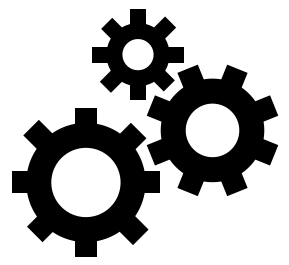
\includegraphics[width=\textwidth,height=0.70833in]{images/03.png} & \begin{minipage}[t]{\linewidth}\raggedright
\textbf{At the end of this chapter you should be able to}

\begin{itemize}
\item
  Understand the 5 most common data structures.
\item
  Understand the data structure lineage.
\item
  Access given subsets of a multi-variable data object.
\end{itemize}
\end{minipage} \\
\end{longtable}

\hfill\break

This book introduced variables briefly in \ref{syntax}. Here, we will expand on that introduction. At its simplest, a variable can be thought of as a container that holds only a single thing, like a single stick of gum. A vector is an ordered, finite collection of variables, like a pack of gum. A matrix consists of columns of equally-sized vectors, similar to a vending machine for several flavors of gum packs. Mentally, you can think of them as a point, a line, and a square, respectively.

\begin{figure}

{\centering 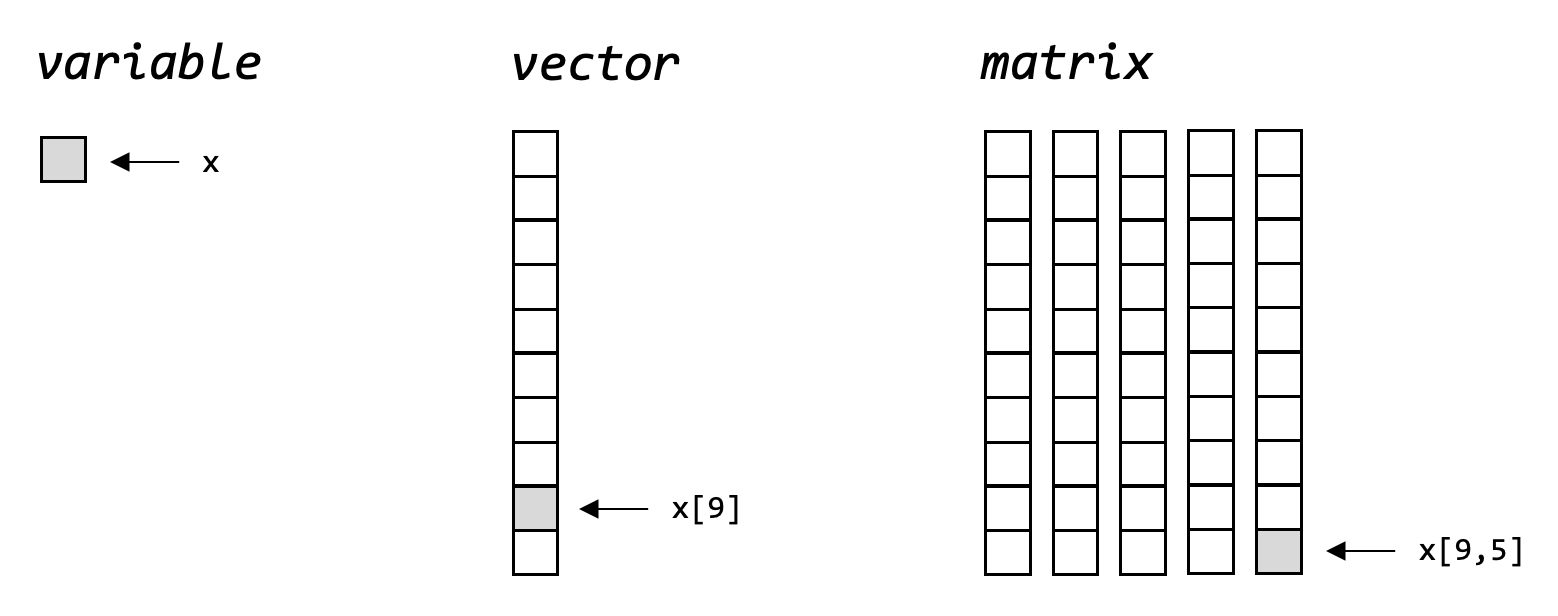
\includegraphics[width=0.67\linewidth]{images/04_001_data_structures} 

}

\caption{\label{fig:4001}R main data structures}\label{fig:4001}
\end{figure}

\hypertarget{variable}{%
\section{Variable}\label{variable}}

Again, a variable is the most basic information container, capable of holding only a single \emph{numeric} or \emph{string} value.

\begin{Shaded}
\begin{Highlighting}[]
\NormalTok{a }\OtherTok{\textless{}{-}} \DecValTok{1}
\end{Highlighting}
\end{Shaded}

\hypertarget{vector}{%
\section{Vector}\label{vector}}

A vector is simply a collection of variables of all the same type. In other programming languages these are called arrays, and can be more permissive allowing for different types of values to be stored together. In R this is not permitted, as vectors can only contain either numbers or strings. If a vector contains a single string value, this ``spoils'' the numbers in the vector, thus making them all strings.

\begin{Shaded}
\begin{Highlighting}[]
\CommentTok{\# permitted}
\NormalTok{a }\OtherTok{\textless{}{-}} \FunctionTok{c}\NormalTok{(}\DecValTok{1}\NormalTok{, }\DecValTok{2}\NormalTok{, }\DecValTok{3}\NormalTok{)}
\NormalTok{a}
\end{Highlighting}
\end{Shaded}

\begin{verbatim}
## [1] 1 2 3
\end{verbatim}

\begin{Shaded}
\begin{Highlighting}[]
\CommentTok{\# the numerical values of 1 and 3 are lost, and now only represented as strings}
\NormalTok{b }\OtherTok{\textless{}{-}} \FunctionTok{c}\NormalTok{(}\DecValTok{1}\NormalTok{, }\StringTok{\textquotesingle{}two\textquotesingle{}}\NormalTok{, }\DecValTok{3}\NormalTok{)}
\NormalTok{b}
\end{Highlighting}
\end{Shaded}

\begin{verbatim}
## [1] "1"   "two" "3"
\end{verbatim}

Vectors can be composed through various methods, either by concatenation with the \texttt{c()} function, as seen above, or using the range operator \texttt{:}. Note that the concatenation method allows for the non-sequential construction of variables, while the range operator constructs a vector of all sequential integers between the two values.

\begin{Shaded}
\begin{Highlighting}[]
\DecValTok{1}\SpecialCharTok{:}\DecValTok{3}
\end{Highlighting}
\end{Shaded}

\begin{verbatim}
## [1] 1 2 3
\end{verbatim}

There are also a handful of pre-populated vectors and functions for constructing patters.

\begin{Shaded}
\begin{Highlighting}[]
\CommentTok{\# all upper case letters}
\NormalTok{LETTERS}
\end{Highlighting}
\end{Shaded}

\begin{verbatim}
##  [1] "A" "B" "C" "D" "E" "F" "G" "H" "I" "J" "K" "L" "M" "N" "O" "P" "Q" "R" "S" "T" "U" "V" "W"
## [24] "X" "Y" "Z"
\end{verbatim}

\begin{Shaded}
\begin{Highlighting}[]
\CommentTok{\# all lower case letters}
\NormalTok{letters}
\end{Highlighting}
\end{Shaded}

\begin{verbatim}
##  [1] "a" "b" "c" "d" "e" "f" "g" "h" "i" "j" "k" "l" "m" "n" "o" "p" "q" "r" "s" "t" "u" "v" "w"
## [24] "x" "y" "z"
\end{verbatim}

\begin{Shaded}
\begin{Highlighting}[]
\CommentTok{\# a repetitive vector of the letter "a"}
\FunctionTok{rep}\NormalTok{(}\StringTok{\textquotesingle{}a\textquotesingle{}}\NormalTok{, }\DecValTok{5}\NormalTok{)}
\end{Highlighting}
\end{Shaded}

\begin{verbatim}
## [1] "a" "a" "a" "a" "a"
\end{verbatim}

\begin{Shaded}
\begin{Highlighting}[]
\CommentTok{\# a repetitive vector of a previous vector}
\FunctionTok{rep}\NormalTok{(b, }\DecValTok{2}\NormalTok{)}
\end{Highlighting}
\end{Shaded}

\begin{verbatim}
## [1] "1"   "two" "3"   "1"   "two" "3"
\end{verbatim}

\begin{Shaded}
\begin{Highlighting}[]
\CommentTok{\# a sequence of integers between two values, in this case reverse order}
\FunctionTok{seq}\NormalTok{(}\DecValTok{10}\NormalTok{, }\DecValTok{5}\NormalTok{)}
\end{Highlighting}
\end{Shaded}

\begin{verbatim}
## [1] 10  9  8  7  6  5
\end{verbatim}

\begin{Shaded}
\begin{Highlighting}[]
\CommentTok{\# same as above}
\DecValTok{10}\SpecialCharTok{:}\DecValTok{5}
\end{Highlighting}
\end{Shaded}

\begin{verbatim}
## [1] 10  9  8  7  6  5
\end{verbatim}

While variables don't require a referencing scheme, because they only contain a single value, vectors need to have some kind of referencing scheme, shown in \ref{fig:4001} as \texttt{x{[}9{]}} and illustrated in the following example.

\hfill\break

\begin{longtable}[]{@{}
  >{\raggedright\arraybackslash}p{(\columnwidth - 2\tabcolsep) * \real{0.1097}}
  >{\raggedright\arraybackslash}p{(\columnwidth - 2\tabcolsep) * \real{0.8903}}@{}}
\toprule\noalign{}
\endhead
\bottomrule\noalign{}
\endlastfoot

\includegraphics[width=\textwidth,height=0.70833in]{images/01.png} & The use of an integer vector to sub-select another vector based on position. R abides by the 1:N positional referencing, where as other programming languages refer to the first vector or array position as 0. \emph{A good topic for a lively discussion with a computer scientist.} \\
\end{longtable}

\hfill\break

\begin{Shaded}
\begin{Highlighting}[]
\NormalTok{x }\OtherTok{\textless{}{-}}\NormalTok{ LETTERS}
\CommentTok{\# 3rd letter in the alphabet}
\NormalTok{x[}\DecValTok{3}\NormalTok{]}
\end{Highlighting}
\end{Shaded}

\begin{verbatim}
## [1] "C"
\end{verbatim}

\begin{Shaded}
\begin{Highlighting}[]
\CommentTok{\# the 9th, 10th, 11th and 12th letters in the alphabet}
\NormalTok{x[}\DecValTok{9}\SpecialCharTok{:}\DecValTok{12}\NormalTok{]}
\end{Highlighting}
\end{Shaded}

\begin{verbatim}
## [1] "I" "J" "K" "L"
\end{verbatim}

\begin{Shaded}
\begin{Highlighting}[]
\CommentTok{\# the 1st, 5th, 10th letters in the alphabet}
\NormalTok{x[}\FunctionTok{c}\NormalTok{(}\DecValTok{1}\NormalTok{,}\DecValTok{5}\NormalTok{,}\DecValTok{10}\NormalTok{)]}
\end{Highlighting}
\end{Shaded}

\begin{verbatim}
## [1] "A" "E" "J"
\end{verbatim}

Numerical vectors can be operated on simultaneously, using the same conventions as variables, imparting convenient utlity to calculating on collections of values.

\begin{Shaded}
\begin{Highlighting}[]
\NormalTok{x }\OtherTok{\textless{}{-}} \DecValTok{1}\SpecialCharTok{:}\DecValTok{10}
\NormalTok{x }\SpecialCharTok{/} \DecValTok{10}
\end{Highlighting}
\end{Shaded}

\begin{verbatim}
##  [1] 0.1 0.2 0.3 0.4 0.5 0.6 0.7 0.8 0.9 1.0
\end{verbatim}

In addition, there are facile ways to extract information using a coonditional statement \ldots{}

\begin{Shaded}
\begin{Highlighting}[]
\NormalTok{x }\OtherTok{\textless{}{-}} \DecValTok{1}\SpecialCharTok{:}\DecValTok{10} \SpecialCharTok{/} \DecValTok{10}
\NormalTok{x }\SpecialCharTok{\textless{}}\NormalTok{ .}\DecValTok{5}
\end{Highlighting}
\end{Shaded}

\begin{verbatim}
##  [1]  TRUE  TRUE  TRUE  TRUE FALSE FALSE FALSE FALSE FALSE FALSE
\end{verbatim}

\ldots{} the \texttt{which()} function returns the integer reference positions for the condition \texttt{x\ \textless{}\ 0.5} \ldots{}

\begin{Shaded}
\begin{Highlighting}[]
\FunctionTok{which}\NormalTok{(x }\SpecialCharTok{\textless{}}\NormalTok{ .}\DecValTok{5}\NormalTok{)}
\end{Highlighting}
\end{Shaded}

\begin{verbatim}
## [1] 1 2 3 4
\end{verbatim}

\ldots{} and since the output of that function is a vector, we can use it to reference the original vector to extract the elements in the vector that satisfy our condition \texttt{x\ \textless{}\ 0.5}.

\begin{Shaded}
\begin{Highlighting}[]
\NormalTok{x[}\FunctionTok{which}\NormalTok{(x }\SpecialCharTok{\textless{}}\NormalTok{ .}\DecValTok{5}\NormalTok{)]}
\end{Highlighting}
\end{Shaded}

\begin{verbatim}
## [1] 0.1 0.2 0.3 0.4
\end{verbatim}

\hypertarget{matrix}{%
\section{Matrix}\label{matrix}}

Building upon the vector, a matrix is simply composed of columns of either all numeric or string vectors. That statement is not completely accurate as matrices can be row based, however, if we mentally orient ourselves to column based organizations, then the following \texttt{data.frame} will make sense. Matrices are constructed using a function as shown in the following example.

\begin{Shaded}
\begin{Highlighting}[]
\CommentTok{\# taking the vector 1:4 and distributing it by 2 rows and 2 columns}
\NormalTok{m }\OtherTok{\textless{}{-}} \FunctionTok{matrix}\NormalTok{(}\DecValTok{1}\SpecialCharTok{:}\DecValTok{4}\NormalTok{,}\DecValTok{2}\NormalTok{,}\DecValTok{2}\NormalTok{)}
\end{Highlighting}
\end{Shaded}

Elements within the matrix have a reference schema similar to vectors, with the first integer in the square brackets is the row and the second the column \texttt{{[}row,col{]}}.

\begin{verbatim}
##      [,1] [,2]
## [1,]    1    3
## [2,]    2    4
\end{verbatim}

Just like a vector, a matrix can be used to compute operations on all elements simultaneously, apply a comparison and extract the variable(s) matching the condition \ldots{}

\begin{Shaded}
\begin{Highlighting}[]
\NormalTok{m\_half }\OtherTok{\textless{}{-}}\NormalTok{ m }\SpecialCharTok{/} \DecValTok{2}
\NormalTok{w\_point5 }\OtherTok{\textless{}{-}} \FunctionTok{which}\NormalTok{(m\_half }\SpecialCharTok{\textgreater{}} \DecValTok{1}\NormalTok{)}
\NormalTok{m[w\_point5]}
\end{Highlighting}
\end{Shaded}

\begin{verbatim}
## [1] 3 4
\end{verbatim}

\ldots{} or more sincintly.

\begin{Shaded}
\begin{Highlighting}[]
\NormalTok{m[}\FunctionTok{which}\NormalTok{(m}\SpecialCharTok{/}\DecValTok{2} \SpecialCharTok{\textgreater{}} \DecValTok{1}\NormalTok{)]}
\end{Highlighting}
\end{Shaded}

\begin{verbatim}
## [1] 3 4
\end{verbatim}

\hypertarget{data-frame}{%
\section{Data Frame}\label{data-frame}}

Tables are one of the fundamental data structures encountered in data analysis, and what separates them from matrices is the mixed use of numerics and strings, and the orientation that \texttt{data.frames} are columns of vectors, with a row association. A table can be cinstructed with the \texttt{data.frame()} function as shown in the example.

\begin{Shaded}
\begin{Highlighting}[]
\NormalTok{df }\OtherTok{\textless{}{-}} \FunctionTok{data.frame}\NormalTok{(}
  \AttributeTok{let =}\NormalTok{ LETTERS,}
  \AttributeTok{pos =} \DecValTok{1}\SpecialCharTok{:}\FunctionTok{length}\NormalTok{(LETTERS)}
\NormalTok{)}
\end{Highlighting}
\end{Shaded}

\begin{verbatim}
##    let pos
## 1    A   1
## 2    B   2
## 3    C   3
## 4    D   4
## 5    E   5
## ...
\end{verbatim}

Lets talk about the structure of what just happened in constructing the \texttt{data.frame} table. Note that we defined the column with \emph{let} and \emph{pos} referring to letter and position, respectively. Second, note the use of the single \texttt{=} to assign a vector to that column rather than the ``out-of-function'' assignment operator \texttt{\textless{}-} -- meaning that functions use the \texttt{=} assignment operator, while data structures use the \texttt{\textless{}-} assignment operator.

The printed output of the \texttt{data.frame} shows the two column headers and also prints out the row names, in this case the integer value. Now, that this table is organized by column with row assiciations, we can perform an evalutaion on one column and reterive the value(s) in the other.

\hypertarget{list}{%
\section{List}\label{list}}

In R programming, a `list' is a powerful and flexible collection of objects of different types. It can contain vectors, matrices, data frames, and even other lists, making it an extremely versatile tool in data analysis, modeling, and visualization.

With its ability to store multiple data types, a list can be used to represent complex structures such as a database table, where each column can be a vector or a matrix. Furthermore, a list can be used to store multiple models for model comparison, or to store a set of parameters for a simulation study.

In addition to its flexibility, a list is also efficient, as it allows for fast and easy data retrieval. It can be used to store large datasets, and its hierarchical structure makes it easy to navigate and manipulate.

Here's an example of how to create a list in R:

\begin{Shaded}
\begin{Highlighting}[]
\CommentTok{\# create a list}
\NormalTok{my\_list }\OtherTok{\textless{}{-}} \FunctionTok{list}\NormalTok{(}\AttributeTok{name =} \StringTok{"Janie R Programmer"}\NormalTok{,}
                \AttributeTok{age =} \DecValTok{32}\NormalTok{,}
                \AttributeTok{salary =} \DecValTok{100000}\NormalTok{,}
                \AttributeTok{interests =} \FunctionTok{c}\NormalTok{(}\StringTok{"coding"}\NormalTok{, }\StringTok{"reading"}\NormalTok{, }\StringTok{"traveling"}\NormalTok{))}

\FunctionTok{print}\NormalTok{(my\_list)}
\end{Highlighting}
\end{Shaded}

\begin{verbatim}
## $name
## [1] "Janie R Programmer"
## 
## $age
## [1] 32
## 
## $salary
## [1] 1e+05
## 
## $interests
## [1] "coding"    "reading"   "traveling"
\end{verbatim}

In the above code, we have created a list `my\_list' with four elements, each having a different data type. The first element `name' is a character vector, the second element `age' is a numeric value, the third element `salary' is also a numeric value, and the fourth element `interests' is a character vector.

We can access the elements of a list using the dollar sign `\$' or double brackets `{[}{[}{]}{]}'. For example:

\begin{Shaded}
\begin{Highlighting}[]
\CommentTok{\# accessing elements of a list}
\FunctionTok{print}\NormalTok{(my\_list}\SpecialCharTok{$}\NormalTok{name)}
\end{Highlighting}
\end{Shaded}

\begin{verbatim}
## [1] "Janie R Programmer"
\end{verbatim}

\begin{Shaded}
\begin{Highlighting}[]
\FunctionTok{print}\NormalTok{(my\_list[[}\StringTok{"salary"}\NormalTok{]])}
\end{Highlighting}
\end{Shaded}

\begin{verbatim}
## [1] 1e+05
\end{verbatim}

Lists are also useful for storing and manipulating complex data structures such as data frames and tibbles.

\hypertarget{tibbles}{%
\section{Tibbles}\label{tibbles}}

A tibble is a modern data frame in R programming language. Tibble is a part of tidyverse package that provides an efficient and user-friendly way to work with data frames. Tibbles are similar to data frames, but they have better printing capabilities, and they are designed to never alter your data.

Tibbles are created using the \texttt{tibble()} function. You can create a tibble by passing vectors, lists, or data frames to the \texttt{tibble()} function. Once created, you can manipulate the tibble using the \texttt{dplyr} package.

\begin{Shaded}
\begin{Highlighting}[]
\FunctionTok{library}\NormalTok{(tidyverse)}

\NormalTok{df }\OtherTok{\textless{}{-}} \FunctionTok{tibble}\NormalTok{(}
  \AttributeTok{let =}\NormalTok{ LETTERS,}
  \AttributeTok{pos =} \DecValTok{1}\SpecialCharTok{:}\FunctionTok{length}\NormalTok{(LETTERS)}
\NormalTok{)}
\end{Highlighting}
\end{Shaded}

\begin{verbatim}
## # A tibble: 26 × 2
##    let     pos
##    <chr> <int>
##  1 A         1
##  2 B         2
##  3 C         3
##  4 D         4
##  5 E         5
##  6 F         6
##  7 G         7
##  8 H         8
##  9 I         9
## 10 J        10
## # … with 16 more rows
## # ℹ Use `print(n = ...)` to see more rows
\end{verbatim}

Tibbles have several advantages over data frames. They print only the first 10 rows and all the columns that fit on the screen. This makes it easier to view and work with large datasets. Tibbles also have better error messages, which makes debugging easier. Additionally, tibbles are more consistent in handling columns with different types of data.

\hypertarget{how-to-tell-what-you-are-dealing-with}{%
\section*{How to tell what you are dealing with}\label{how-to-tell-what-you-are-dealing-with}}
\addcontentsline{toc}{section}{How to tell what you are dealing with}

You can use the \texttt{str()} function to peak inside any data object to see how it is structured.

The contents of a data.frame:

\begin{Shaded}
\begin{Highlighting}[]
\NormalTok{plant\_data }\OtherTok{\textless{}{-}} \FunctionTok{data.frame}\NormalTok{(}
  \AttributeTok{age\_days =} \FunctionTok{c}\NormalTok{(}\DecValTok{10}\NormalTok{, }\DecValTok{20}\NormalTok{, }\DecValTok{30}\NormalTok{, }\DecValTok{40}\NormalTok{, }\DecValTok{50}\NormalTok{, }\DecValTok{60}\NormalTok{),}
  \AttributeTok{height\_inch =} \FunctionTok{c}\NormalTok{(}\FloatTok{1.02}\NormalTok{, }\FloatTok{1.10}\NormalTok{, }\FloatTok{5.10}\NormalTok{, }\FloatTok{6.00}\NormalTok{, }\FloatTok{6.50}\NormalTok{, }\FloatTok{6.90}\NormalTok{)}
\NormalTok{)}

\FunctionTok{str}\NormalTok{(plant\_data)}
\end{Highlighting}
\end{Shaded}

\begin{verbatim}
## 'data.frame':    6 obs. of  2 variables:
##  $ age_days   : num  10 20 30 40 50 60
##  $ height_inch: num  1.02 1.1 5.1 6 6.5 6.9
\end{verbatim}

The contents of a tibble is very similar:

\begin{Shaded}
\begin{Highlighting}[]
\NormalTok{plant\_data }\OtherTok{\textless{}{-}} \FunctionTok{tibble}\NormalTok{(}
  \AttributeTok{age\_days =} \FunctionTok{c}\NormalTok{(}\DecValTok{10}\NormalTok{, }\DecValTok{20}\NormalTok{, }\DecValTok{30}\NormalTok{, }\DecValTok{40}\NormalTok{, }\DecValTok{50}\NormalTok{, }\DecValTok{60}\NormalTok{),}
  \AttributeTok{height\_inch =} \FunctionTok{c}\NormalTok{(}\FloatTok{1.02}\NormalTok{, }\FloatTok{1.10}\NormalTok{, }\FloatTok{5.10}\NormalTok{, }\FloatTok{6.00}\NormalTok{, }\FloatTok{6.50}\NormalTok{, }\FloatTok{6.90}\NormalTok{)}
\NormalTok{)}

\FunctionTok{str}\NormalTok{(plant\_data)}
\end{Highlighting}
\end{Shaded}

\begin{verbatim}
## tibble [6 x 2] (S3: tbl_df/tbl/data.frame)
##  $ age_days   : num [1:6] 10 20 30 40 50 60
##  $ height_inch: num [1:6] 1.02 1.1 5.1 6 6.5 6.9
\end{verbatim}

The contents of a linear regression data object are quite different:

\begin{Shaded}
\begin{Highlighting}[]
\CommentTok{\# linear prediction of plant growth (eg. height) based on age}
\NormalTok{linear\_model }\OtherTok{\textless{}{-}} \FunctionTok{lm}\NormalTok{(}\AttributeTok{data =}\NormalTok{ plant\_data, height\_inch }\SpecialCharTok{\textasciitilde{}}\NormalTok{ age\_days)}

\NormalTok{linear\_model}
\end{Highlighting}
\end{Shaded}

\begin{verbatim}
## 
## Call:
## lm(formula = height_inch ~ age_days, data = plant_data)
## 
## Coefficients:
## (Intercept)     age_days  
##     -0.2133       0.1329
\end{verbatim}

\begin{Shaded}
\begin{Highlighting}[]
\FunctionTok{str}\NormalTok{(linear\_model)}
\end{Highlighting}
\end{Shaded}

\begin{verbatim}
List of 12
 $ coefficients : Named num [1:2] -0.213 0.133
  ..- attr(*, "names")= chr [1:2] "(Intercept)" "age_days"
 $ residuals    : Named num [1:6] -0.0952 -1.3438 1.3276 0.899 0.0705 ...
  ..- attr(*, "names")= chr [1:6] "1" "2" "3" "4" ...
 $ effects      : Named num [1:6] -10.868 5.558 1.296 0.602 -0.492 ...
  ..- attr(*, "names")= chr [1:6] "(Intercept)" "age_days" "" "" ...
 $ rank         : int 2
 $ fitted.values: Named num [1:6] 1.12 2.44 3.77 5.1 6.43 ...
  ..- attr(*, "names")= chr [1:6] "1" "2" "3" "4" ...
\end{verbatim}

\hypertarget{exercises-2}{%
\section*{Exercises}\label{exercises-2}}
\addcontentsline{toc}{section}{Exercises}

\begin{longtable}[]{@{}
  >{\raggedright\arraybackslash}p{(\columnwidth - 2\tabcolsep) * \real{0.3036}}
  >{\raggedright\arraybackslash}p{(\columnwidth - 2\tabcolsep) * \real{0.6964}}@{}}
\toprule\noalign{}
\endhead
\bottomrule\noalign{}
\endlastfoot

\includegraphics[width=\textwidth,height=0.70833in]{images/07.png} & \begin{minipage}[t]{\linewidth}\raggedright
\begin{itemize}
\item
  Create a new R Studio Project and name it \textbf{003\_data\_structures}.
\item
  Create a new R script, add your name and date at the top as comments.
\end{itemize}
\end{minipage} \\
\end{longtable}

\begin{enumerate}
\def\labelenumi{\arabic{enumi}.}
\tightlist
\item
  Construct the following vector and store as a variable.
\end{enumerate}

\begin{verbatim}
## [1] "red"   "green" "blue"
\end{verbatim}

\begin{enumerate}
\def\labelenumi{\arabic{enumi}.}
\setcounter{enumi}{1}
\tightlist
\item
  Extract the 2nd element in the variable.
\end{enumerate}

\begin{verbatim}
## [1] "green"
\end{verbatim}

\begin{enumerate}
\def\labelenumi{\arabic{enumi}.}
\setcounter{enumi}{2}
\tightlist
\item
  Construct a numerical vector of length 5, containing the diameters of circles with integer circumferences 1 to 5. Remember PEMDAS.
\end{enumerate}

\begin{verbatim}
## [1]  3.141593 12.566372 28.274337 50.265488 78.539825
\end{verbatim}

\begin{enumerate}
\def\labelenumi{\arabic{enumi}.}
\setcounter{enumi}{3}
\tightlist
\item
  Extract all circumferences greater than 50.
\end{enumerate}

\begin{verbatim}
## [1] 50.26549 78.53982
\end{verbatim}

\hypertarget{tidyverse-1}{%
\chapter{Tidyverse}\label{tidyverse-1}}

The \texttt{tidyverse} is actually a collection of R packages designed for data analysis and visualization. It is an essential tool for data scientists and statisticians who work with large datasets.

\hfill\break

\begin{longtable}[]{@{}
  >{\raggedright\arraybackslash}p{(\columnwidth - 2\tabcolsep) * \real{0.3617}}
  >{\raggedright\arraybackslash}p{(\columnwidth - 2\tabcolsep) * \real{0.6383}}@{}}
\toprule\noalign{}
\endhead
\bottomrule\noalign{}
\endlastfoot
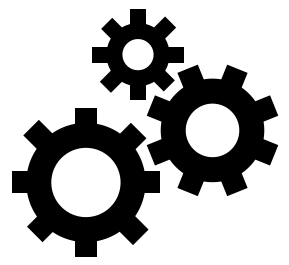
\includegraphics[width=\textwidth,height=0.70833in]{images/03.png} & \begin{minipage}[t]{\linewidth}\raggedright
\textbf{At the end of this chapter you should be able to}

\begin{itemize}
\item
  Grasp the utility of the tidyverse.
\item
  Understand how to construct a data pipeline.
\item
  Composed a simple workflow.
\end{itemize}
\end{minipage} \\
\end{longtable}

\hfill\break

The \texttt{tidyverse} packages are built around a common philosophy of data manipulation. The goal is to provide a consistent and intuitive syntax for data analysis that is easy to learn and use. The packages in the \texttt{tidyverse} include:

\begin{longtable}[]{@{}
  >{\raggedright\arraybackslash}p{(\columnwidth - 2\tabcolsep) * \real{0.3563}}
  >{\raggedright\arraybackslash}p{(\columnwidth - 2\tabcolsep) * \real{0.6437}}@{}}
\toprule\noalign{}
\endhead
\bottomrule\noalign{}
\endlastfoot
\ref{magrittr} magrittr & provides the pipe, \%\textgreater\% used throughout the tidyverse. \\
\ref{tibble} tibble & creates the main data object. \\
\ref{readr} readr & reading and writing data in various formats. \\
\ref{dplyr} dplyr & data manipulation. \\
\ref{tidyr} tidyr & transforming messy data into a tidy format. \\
\ref{purrr} purrr & functional programming with vectors and lists. \\
\ref{stringr} stringr & working with strings. \\
\ref{lubridate} lubridate & working with dates and date strings. \\
\ref{ggplot2} ggplot2 & graphical plotting and data visualization. \\
\end{longtable}

These packages work seamlessly together, allowing users to easily manipulate and visualize their data. The \texttt{tidyverse} also includes a set of conventions and best practices for data analysis, making it easy to follow a consistent workflow.

\hfill\break

\begin{longtable}[]{@{}
  >{\raggedright\arraybackslash}p{(\columnwidth - 2\tabcolsep) * \real{0.3617}}
  >{\raggedright\arraybackslash}p{(\columnwidth - 2\tabcolsep) * \real{0.6383}}@{}}
\toprule\noalign{}
\endhead
\bottomrule\noalign{}
\endlastfoot

\includegraphics[width=\textwidth,height=0.70833in]{images/01.png} & \textbf{Cheat-sheets} \ref{cheat-sheets} \\
\end{longtable}

\hfill\break

Consider the following workflow to read in data, calculate a linear regression and visualize the data using nine (9) of the underlying packages in the tidyverse.

\begin{Shaded}
\begin{Highlighting}[]
\FunctionTok{library}\NormalTok{(tidyverse)}

\CommentTok{\# readr, tibble, magrittr: read in a table of comma separate values}
\NormalTok{tbl\_csv }\OtherTok{\textless{}{-}} \StringTok{"data/denver\_climate.csv"} \SpecialCharTok{\%\textgreater{}\%} \FunctionTok{read\_csv}\NormalTok{()}

\CommentTok{\# define a function to fit a linear regression model}
\NormalTok{lm\_func }\OtherTok{\textless{}{-}} \ControlFlowTok{function}\NormalTok{(data) \{}
  \FunctionTok{lm}\NormalTok{(snowfall }\SpecialCharTok{\textasciitilde{}}\NormalTok{ min\_temp, }\AttributeTok{data =}\NormalTok{ data)}
\NormalTok{\}}

\CommentTok{\# readr, tibble, magrittr: using the data imported from above}
\NormalTok{tbl\_csv\_lm }\OtherTok{\textless{}{-}}\NormalTok{ tbl\_csv }\SpecialCharTok{\%\textgreater{}\%}
  \CommentTok{\# dplyr}
  \FunctionTok{group\_by}\NormalTok{(year) }\SpecialCharTok{\%\textgreater{}\%}
  \CommentTok{\# tidyr}
  \FunctionTok{nest}\NormalTok{() }\SpecialCharTok{\%\textgreater{}\%}
  \CommentTok{\# dplyr, purrr: apply the function to each nested data frame}
  \FunctionTok{mutate}\NormalTok{(}\AttributeTok{model =} \FunctionTok{map}\NormalTok{(data, lm\_func)) }\SpecialCharTok{\%\textgreater{}\%}
  \CommentTok{\# dplyr, broom, purrr: extract the coefficients from each model}
  \FunctionTok{mutate}\NormalTok{(}\AttributeTok{tidy =} \FunctionTok{map}\NormalTok{(model, broom}\SpecialCharTok{::}\NormalTok{tidy)) }\SpecialCharTok{\%\textgreater{}\%}
  \CommentTok{\# tidyr}
  \FunctionTok{unnest}\NormalTok{(tidy) }\SpecialCharTok{\%\textgreater{}\%}
  \CommentTok{\# dplyr, stringr}
  \FunctionTok{mutate}\NormalTok{(}\AttributeTok{term =}\NormalTok{ term }\SpecialCharTok{\%\textgreater{}\%} \FunctionTok{str\_replace\_all}\NormalTok{(}\StringTok{"}\SpecialCharTok{\textbackslash{}\textbackslash{}}\StringTok{(|}\SpecialCharTok{\textbackslash{}\textbackslash{}}\StringTok{)"}\NormalTok{, }\StringTok{""}\NormalTok{)) }\SpecialCharTok{\%\textgreater{}\%}
  \CommentTok{\# dplyr: retain only specific columns}
  \FunctionTok{select}\NormalTok{(year, term, estimate) }\SpecialCharTok{\%\textgreater{}\%}
  \CommentTok{\# tidyr: convert from a long table to a wide table}
  \FunctionTok{pivot\_wider}\NormalTok{(}\AttributeTok{names\_from =} \StringTok{\textquotesingle{}term\textquotesingle{}}\NormalTok{, }\AttributeTok{values\_from =} \StringTok{\textquotesingle{}estimate\textquotesingle{}}\NormalTok{)}


\CommentTok{\#ggplot2}
\NormalTok{tbl\_csv }\SpecialCharTok{\%\textgreater{}\%}
  \FunctionTok{ggplot}\NormalTok{(}\FunctionTok{aes}\NormalTok{(min\_temp, snowfall)) }\SpecialCharTok{+} 
  \FunctionTok{geom\_point}\NormalTok{() }\SpecialCharTok{+}
  \CommentTok{\# use the linear model data to plot regression lines}
  \FunctionTok{geom\_abline}\NormalTok{(}\AttributeTok{data =}\NormalTok{ tbl\_csv\_lm,}
              \FunctionTok{aes}\NormalTok{(}\AttributeTok{slope =}\NormalTok{ min\_temp, }\AttributeTok{intercept =}\NormalTok{ Intercept)) }\SpecialCharTok{+}
  \CommentTok{\# plot each year separately }
  \FunctionTok{facet\_wrap}\NormalTok{(}\SpecialCharTok{\textasciitilde{}}\NormalTok{year)}
\end{Highlighting}
\end{Shaded}

\begin{center}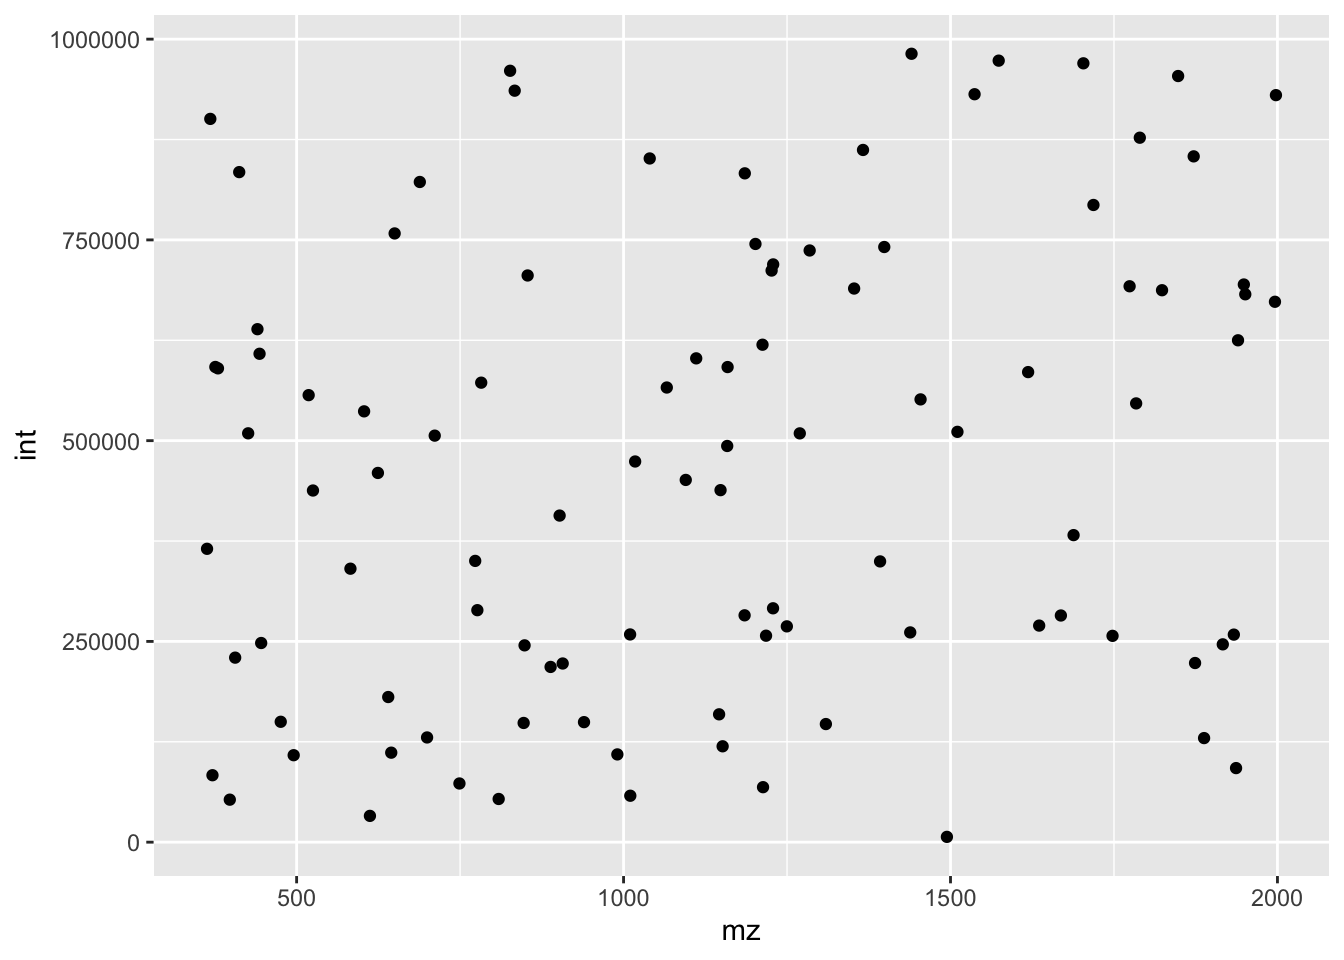
\includegraphics{_main_files/figure-latex/unnamed-chunk-66-1} \end{center}

To get started with the \texttt{tidyverse}, you can install the package using the following command:

\begin{Shaded}
\begin{Highlighting}[]
\FunctionTok{install.packages}\NormalTok{(}\StringTok{"tidyverse"}\NormalTok{)}
\end{Highlighting}
\end{Shaded}

Once installed, users can load the package and begin using the individual packages within the tidyverse:

\begin{Shaded}
\begin{Highlighting}[]
\FunctionTok{library}\NormalTok{(tidyverse)}
\end{Highlighting}
\end{Shaded}

Overall, the tidyverse is an essential tool for data analysis and visualization in R. Its user-friendly syntax and consistent conventions make it easy for data scientists and statisticians to work with large datasets.

\hypertarget{core-packages}{%
\section{Core Packages}\label{core-packages}}

Two important packages in the tidyverse are tibble and magrittr. These core packages enable other data manipulation operations to work seamlessly, improving efficiency and ease of use when working with data in R. Despite their importance, they are often taken for granted.

\hypertarget{magrittr}{%
\subsection{magrittr}\label{magrittr}}

The tidyverse package \texttt{magrittr} is a popular R package that provides a set of operators for chaining operations in a sequence. The package was developed by Stefan Milton Bache and Hadley Wickham. The main goal of \texttt{magrittr} is to make code more readable and easier to maintain.

The pipe operator, \texttt{\%\textgreater{}\%}, is the most famous operator provided by \texttt{magrittr.} It allows you to chain multiple operations without the need to use intermediate variables. The pipe operator takes the output of the previous function and passes it as the first argument to the next function. This chaining of operations allows for more concise and readable code.

Here is an example of how to use the pipe operator with \texttt{magrittr}:

\begin{Shaded}
\begin{Highlighting}[]
\CommentTok{\# create a vector of numbers}
\NormalTok{numbers }\OtherTok{\textless{}{-}} \FunctionTok{c}\NormalTok{(}\DecValTok{1}\NormalTok{, }\DecValTok{2}\NormalTok{, }\DecValTok{3}\NormalTok{, }\DecValTok{4}\NormalTok{, }\DecValTok{5}\NormalTok{)}

\CommentTok{\# use the pipe operator to chain operations}
\NormalTok{numbers }\SpecialCharTok{\%\textgreater{}\%}
  \FunctionTok{sum}\NormalTok{() }\SpecialCharTok{\%\textgreater{}\%}
  \FunctionTok{sqrt}\NormalTok{()}
\end{Highlighting}
\end{Shaded}

\begin{verbatim}
## [1] 3.872983
\end{verbatim}

In this example, we create a vector of numbers and use the pipe operator to chain the \texttt{sum()} and \texttt{sqrt()} functions. The output of the \texttt{sum()} function is passed as the first argument to the \texttt{sqrt()} function. This allows us to calculate the sum and square root of the vector in a single line of code.

Magrittr also provides other useful operators, such as the assignment pipe \texttt{\%\textless{}\textgreater{}\%}, which allows you to update a variable in place, and the tee operator \texttt{\%T\textgreater{}\%}, which allows you to inspect the output of an operation without interrupting the chain.

\hypertarget{tibble}{%
\subsection{tibble}\label{tibble}}

R \texttt{tibble} is a class of data frame in the R programming language. It is an improved alternative to the traditional data frame and is part of the tidyverse package. Tibbles are data frames with stricter requirements, and they provide a streamlined and more efficient way to work with data.

One of the main advantages of tibbles is that they provide a cleaner and more consistent way to display data. Tibbles only show the first 10 rows and all the columns that fit on the screen, making it easier to work with large datasets. Additionally, tibbles automatically convert character vectors to factors, preventing common errors that can occur when working with data frames.

Another important feature of tibbles is the way they handle column names. Tibbles will not allow spaces in column names, and they use backticks to reference columns with non-standard names. This makes it easier to work with datasets that have complex column names. Tibbles also provide a more consistent way to handle missing values. In data frames, missing values can be represented in different ways, such as NA, NaN, or NULL. Tibbles, on the other hand, only use NA to represent missing values, making it easier to work with missing data.

\hypertarget{importing}{%
\section{Importing}\label{importing}}

\hypertarget{readr}{%
\subsection{readr}\label{readr}}

R \texttt{readr} is a package in the R language that is used to read structured data files into R. The package is an efficient and user-friendly toolkit that allows for the reading of different types of flat files such as CSV, TSV, and fixed-width files. It is part of the tidyverse collection of packages, which is popular among data scientists and statisticians.

One of the key features of \texttt{readr} is its ability to quickly read data into R, making it an ideal package for data analysis and data cleaning. \texttt{readr} is designed to handle various types of data, including numeric, date, and character data. The package also has advanced features such as automatic guessing of column types, encoding detection, and parsing of dates and times.

\begin{Shaded}
\begin{Highlighting}[]
\CommentTok{\# read comma separated values}
\NormalTok{tbl\_csv }\OtherTok{\textless{}{-}} \StringTok{"data/denver\_climate.csv"} \SpecialCharTok{\%\textgreater{}\%} \FunctionTok{read\_csv}\NormalTok{()}
\end{Highlighting}
\end{Shaded}

One of the best things about \texttt{readr} is its consistency in dealing with file formats, which allows for easy and fast data manipulation. The package provides a high level of control over the import process, allowing you to specify the location of the data file, the delimiter, and the encoding type. Additionally, \texttt{readr} can handle large datasets with ease, making it one of the most efficient packages for data handling.

\hypertarget{wrangling}{%
\section{Wrangling}\label{wrangling}}

\hypertarget{dplyr}{%
\subsection{dplyr}\label{dplyr}}

R \texttt{dplyr} is perhaps pne of the most powerful libraries in the \texttt{tidyverse}, providing a set of tools for data manipulation and transformation. It is designed to work seamlessly with data stored in data frames.

The library comes with a set of functions that can be used to filter, arrange, group, mutate, and summarize data. These functions are optimized for speed and memory efficiency, allowing users to work with large datasets easily.

Some of the most commonly used functions in \texttt{dplyr} are:

\begin{itemize}
\tightlist
\item
  \textbf{filter}: used to extract specific rows from a data frame based on certain conditions.
\item
  \textbf{arrange}: used to sort the rows of a data frame based on one or more columns.
\item
  \textbf{select}: used to select specific columns from a data frame.
\item
  \textbf{mutate}: used to add new columns to a data frame.
\end{itemize}

In addition to these functions, dplyr also includes a set of convenient shortcuts and helpers, such as the pipe operator (\%\textgreater\%) which allows users to chain multiple operations together in a more intuitive and readable way.

\hypertarget{tidyr}{%
\subsection{tidyr}\label{tidyr}}

R \texttt{tidyr} is a package in R that helps to reshape data frames. It is an essential tool for data cleaning and analysis. Tidyr is used to convert data from wide to long format and vice versa, and it also helps to separate and unite columns.

\begin{itemize}
\tightlist
\item
  \textbf{pivot\_longer}: used to reshape data from a column-based wide format to a row-based long format.
\item
  \textbf{pivot\_wider}: used to reshape data from a row-based long format to a column-based wide format.
\end{itemize}

The package \texttt{tidyr} also has functions to separate and unite columns. The ``separate'' function is used when you have a column that contains multiple variables. For example, if you have a column that contains both the first and last name of a person, you can separate them into two columns. The ``unite'' function is the opposite of separate. It is used when you want to combine two or more columns into one column.

\begin{itemize}
\tightlist
\item
  \textbf{seperate}: used to separate a column with multiple values into two or more columns.
\item
  \textbf{seperate\_row}: used to duplicate a row with multiple values from a given column.
\end{itemize}

\hypertarget{purrr}{%
\subsection{purrr}\label{purrr}}

The \texttt{purrr} package is a functional programming toolkit for R that enables users to easily and rapidly apply a function to a set of inputs, returning a list or vector of outputs. It is designed to work seamlessly with the tidyverse ecosystem of packages, but can also be used with base R functions.

The most important feature in \texttt{purrr} is its ability to replace loops with functions that save time and effort. The package has a collection of functions that allow you to work with functions that take one or more arguments. Some of these functions include \texttt{map}, \texttt{map2}, \texttt{pmap}, and \texttt{imap.}

The map function is purrr's flagship function and is used to apply a function to each element of a list or vector, returning a list of outputs. The \texttt{map2} function applies a function to two lists or vectors in parallel, returning a list of outputs. The \texttt{pmap} function applies a function to an arbitrary number of lists or vectors in parallel, returning a list of outputs. The \texttt{imap} function is similar to map, but also provides the index of the current element in the input vector.

Purrr also includes features such as the possibility of mapping over nested lists, using \texttt{map} and variants to iterate over grouped data, and using \texttt{map} and variants to modify data in place.

\begin{Shaded}
\begin{Highlighting}[]
\NormalTok{numbers }\OtherTok{\textless{}{-}} \FunctionTok{list}\NormalTok{(}\DecValTok{1}\NormalTok{, }\DecValTok{2}\NormalTok{, }\DecValTok{3}\NormalTok{, }\DecValTok{4}\NormalTok{, }\DecValTok{5}\NormalTok{)}

\CommentTok{\# define a function to square a number}
\NormalTok{square }\OtherTok{\textless{}{-}} \ControlFlowTok{function}\NormalTok{(x) \{ x }\SpecialCharTok{\^{}} \DecValTok{2}\NormalTok{ \}}

\CommentTok{\# use map to apply the function to each element of the list}
\NormalTok{squared\_numbers }\OtherTok{\textless{}{-}} \FunctionTok{map}\NormalTok{(numbers, square)}

\CommentTok{\# print the result}
\NormalTok{squared\_numbers}
\end{Highlighting}
\end{Shaded}

\begin{verbatim}
## [[1]]
## [1] 1
## 
## [[2]]
## [1] 4
## 
## [[3]]
## [1] 9
## 
## [[4]]
## [1] 16
## 
## [[5]]
## [1] 25
\end{verbatim}

\hypertarget{glue}{%
\subsection{glue}\label{glue}}

R \texttt{glue} is a tidyverse package that provides a simple way to interpolate values into strings. It allows users to combine multiple strings or variables together into a single string with minimum efforts, simpler than using base R fuctions.

The \texttt{glue} function can handle various types of inputs, including vectors, lists, and expressions. It also supports user-defined formats and allows users to specify separators between the values.

One of the significant advantages of using \texttt{glue} is that it provides a more readable and concise way to create strings in R. It eliminates the need for multiple \texttt{paste()} or \texttt{paste0()} statements, which can be cumbersome and error-prone.

For example, instead of writing:

\begin{Shaded}
\begin{Highlighting}[]
\FunctionTok{paste0}\NormalTok{(}\StringTok{"The value of x is: "}\NormalTok{, x, }\StringTok{", and the value of y is: "}\NormalTok{, y)}
\end{Highlighting}
\end{Shaded}

we can use R glue:

\begin{Shaded}
\begin{Highlighting}[]
\FunctionTok{glue}\NormalTok{(}\StringTok{"The value of x is: \{x\}, and the value of y is: \{y\}"}\NormalTok{)}
\end{Highlighting}
\end{Shaded}

This code will produce the same output, but it's more readable and easier to modify.

\hypertarget{data-types}{%
\section{Data Types}\label{data-types}}

\hypertarget{stringr}{%
\subsection{stringr}\label{stringr}}

The tidyverse package \texttt{stringr} provides a cohesive set of functions designed to make working with strings more efficient. It is especially useful when dealing with messy or unstructured data that needs to be cleaned and transformed into a more structured format.

Several functions in \texttt{stringr} provides methods working with strings, for example:

\begin{itemize}
\tightlist
\item
  \textbf{str\_replace}: replaces a pattern with another pattern in a string.
\end{itemize}

\begin{Shaded}
\begin{Highlighting}[]
\FunctionTok{str\_replace}\NormalTok{(}\StringTok{"Hello World"}\NormalTok{, }\StringTok{"W.+"}\NormalTok{, }\StringTok{"Everyone"}\NormalTok{)}
\end{Highlighting}
\end{Shaded}

\begin{verbatim}
## [1] "Hello Everyone"
\end{verbatim}

\begin{itemize}
\tightlist
\item
  \textbf{str\_extract}: extracts the first occurrence of a pattern from a string.
\end{itemize}

\begin{Shaded}
\begin{Highlighting}[]
\FunctionTok{str\_extract}\NormalTok{(}\StringTok{"Hello World"}\NormalTok{, }\StringTok{"W.+"}\NormalTok{)}
\end{Highlighting}
\end{Shaded}

\begin{verbatim}
## [1] "World"
\end{verbatim}

\begin{itemize}
\tightlist
\item
  \textbf{str\_split}: splits a string into pieces based on a specified pattern.
\end{itemize}

\begin{Shaded}
\begin{Highlighting}[]
\FunctionTok{str\_split}\NormalTok{(}\StringTok{"Hello World"}\NormalTok{, }\StringTok{"}\SpecialCharTok{\textbackslash{}\textbackslash{}}\StringTok{s"}\NormalTok{)}
\end{Highlighting}
\end{Shaded}

\begin{verbatim}
## [[1]]
## [1] "Hello" "World"
\end{verbatim}

\hypertarget{lubridate}{%
\subsection{lubridate}\label{lubridate}}

The tidyverse package \texttt{lubridate} helps with the handling of dates and times. The package has several functions that make it easier to work with dates and times, especially when dealing with data that has different formats.

Some of the functions in \texttt{lubridate} package include:

\begin{itemize}
\tightlist
\item
  \textbf{ymd} - this is used to convert dates in the format of year, month, and day to the date format in R. For example, \texttt{ymd("20220101")} will return the date in R format.
\item
  \textbf{dmy} - this is used to convert dates in the format of day, month, and year to the date format in R. For example, \texttt{dmy("01-01-2022")} will return the date in R format.
\item
  \textbf{hms} - this is used to convert time in the format of hours, minutes, and seconds to the time format in R. For example, \texttt{hms("12:30:15")} will return the time in R format.
\item
  \textbf{ymd\_hms} - this is used to convert dates and times in the format of year, month, day, hours, minutes, and seconds to the date and time format in R. For example, \texttt{ymd\_hms("2022-01-01\ 12:30:15")} will return the date and time in R format.
\end{itemize}

There are also functions for extracting information from dates and times such as \texttt{year()}, \texttt{month()}, \texttt{day()}, \texttt{hour()}, \texttt{minute()}, and \texttt{second()}.

\hypertarget{forcats}{%
\subsection{forcats}\label{forcats}}

R \texttt{forcats} is a tidyverse package that provides a set of tools for working with categorical data. It is designed to make it easier to work with factors in R, which are used to represent categorical data.

The \texttt{forcats} package provides several functions that can be used to manipulate factors, including reordering levels, combining levels, and handling missing values. It also provides functions for working with ordered factors, which are used to represent data that has a natural ordering, such as age groups or ratings.

One of the key benefits of using \texttt{forcats} is that it allows you to easily visualize and analyze categorical data. The package provides functions for creating categorical plots, such as bar charts and pie charts, as well as for calculating summary statistics for categorical data.

In addition to its core functionality, \texttt{forcats} is also highly customizable. It provides a wide range of options for controlling the appearance of plots and for customizing the behavior of factor manipulation functions.

\hypertarget{summarizing}{%
\section{Summarizing}\label{summarizing}}

\hypertarget{dplyr-1}{%
\subsection{dplyr}\label{dplyr-1}}

In the R tidyverse package, summarizing data is a common task performed on data frames. The dplyr package provides a set of functions that makes it easy to summarize data based on one or more variables.

\begin{itemize}
\tightlist
\item
  \textbf{group\_by}: used to group rows of a data frame by one or more columns.
\item
  \textbf{summarize}: used to summarize the data based on one or more aggregate functions.
\end{itemize}

The summarise() function is used to perform simple summary statistics on data frames. It takes the name of the new variable as well as the summary function that should be used to calculate its value. For example, to calculate the mean and standard deviation of a variable named `x' in a data frame named `df', we can use the following code:

\begin{Shaded}
\begin{Highlighting}[]
\NormalTok{tbl\_csv }\SpecialCharTok{\%\textgreater{}\%}
  \FunctionTok{summarise}\NormalTok{(}\AttributeTok{mean =} \FunctionTok{mean}\NormalTok{(precipitation), }
            \AttributeTok{sd =} \FunctionTok{sd}\NormalTok{(precipitation))}
\end{Highlighting}
\end{Shaded}

\begin{verbatim}
## # A tibble: 1 x 2
##    mean    sd
##   <dbl> <dbl>
## 1  1.29  1.32
\end{verbatim}

The group\_by() function is used to group data frames by one or more variables. This is useful when we want to summarize data by different categories. For example, to calculate the mean and standard deviation of `x' by `group', we can use the following code:

\begin{Shaded}
\begin{Highlighting}[]
\NormalTok{tbl\_csv }\SpecialCharTok{\%\textgreater{}\%}
  \FunctionTok{group\_by}\NormalTok{(year) }\SpecialCharTok{\%\textgreater{}\%}
  \FunctionTok{summarise}\NormalTok{(}\AttributeTok{mean =} \FunctionTok{mean}\NormalTok{(precipitation), }
            \AttributeTok{sd =} \FunctionTok{sd}\NormalTok{(precipitation))}
\end{Highlighting}
\end{Shaded}

\begin{verbatim}
## # A tibble: 4 x 3
##    year  mean    sd
##   <dbl> <dbl> <dbl>
## 1  2016  1.32 1.29 
## 2  2017  1.43 1.85 
## 3  2018  1.03 1.16 
## 4  2019  1.37 0.945
\end{verbatim}

The summarize\_at() and summarize\_all() functions are used to perform summary statistics on multiple variables at once. The summarize\_at() function takes a list of variables to summarize, while the summarize\_all() function summarizes all variables in the data frame. For example, to calculate the mean and standard deviation of all numeric variables in a data frame named `df', we can use the following code:

\begin{Shaded}
\begin{Highlighting}[]
\NormalTok{tbl\_csv }\SpecialCharTok{\%\textgreater{}\%}
  \FunctionTok{summarise\_all}\NormalTok{(}\FunctionTok{list}\NormalTok{(}\AttributeTok{mean =}\NormalTok{ mean, }\AttributeTok{sd =}\NormalTok{ sd))}
\end{Highlighting}
\end{Shaded}

\begin{verbatim}
## # A tibble: 1 x 12
##   year_mean month~1 max_t~2 min_t~3 preci~4 snowf~5 year_sd month~6 max_t~7 min_t~8 preci~9 snowf~*
##       <dbl>   <dbl>   <dbl>   <dbl>   <dbl>   <dbl>   <dbl>   <dbl>   <dbl>   <dbl>   <dbl>   <dbl>
## 1     2018.     6.5    64.6    36.6    1.29    4.09    1.13    3.49    15.2    14.2    1.32    5.75
## # ... with abbreviated variable names 1: month_mean, 2: max_temp_mean, 3: min_temp_mean,
## #   4: precipitation_mean, 5: snowfall_mean, 6: month_sd, 7: max_temp_sd, 8: min_temp_sd,
## #   9: precipitation_sd, *: snowfall_sd
\end{verbatim}

Summarizing data is an essential task that can be performed using several functions. These functions make it easy to calculate summary statistics based on one or more variables, group data frames by different categories, and summarize multiple variables at once.

\hypertarget{ggplot2}{%
\subsection{ggplot2}\label{ggplot2}}

The tidyverse package \texttt{ggplot2}, demonstrated at the onset of this chapter, is a data visualization package in R programming language that provides a flexible and powerful framework for creating graphs and charts. It is built on the grammar of graphics, which is a systematic way of mapping data to visual elements like points, lines, and bars.

With \texttt{ggplot2}, you can create a wide range of graphs including scatterplots, bar charts, line charts, and more. The package offers a variety of customization options, such as color schemes, themes, and annotations, allowing you to create professional-looking visualizations with ease.

One of the key benefits of \texttt{ggplot2} is that it allows you to quickly explore and analyze your data visually. You can easily create multiple graphs with different variables and subsets of your data, and compare them side by side to identify patterns and trends.

\hypertarget{exercises-3}{%
\section*{Exercises}\label{exercises-3}}
\addcontentsline{toc}{section}{Exercises}

\begin{longtable}[]{@{}
  >{\raggedright\arraybackslash}p{(\columnwidth - 2\tabcolsep) * \real{0.3036}}
  >{\raggedright\arraybackslash}p{(\columnwidth - 2\tabcolsep) * \real{0.6964}}@{}}
\toprule\noalign{}
\endhead
\bottomrule\noalign{}
\endlastfoot

\includegraphics[width=\textwidth,height=0.70833in]{images/07.png} & \begin{minipage}[t]{\linewidth}\raggedright
\begin{itemize}
\item
  Create a new R Studio Project and name it \textbf{004\_tidyverse}.
\item
  Create a new R script, add your name and date at the top as comments.
\end{itemize}
\end{minipage} \\
\end{longtable}

\begin{enumerate}
\def\labelenumi{\arabic{enumi}.}
\tightlist
\item
  Calculate the mean of following vector.
\end{enumerate}

\begin{verbatim}
##  [1]  7.48 14.15  6.23 10.21 15.13  8.19  8.58  8.09  9.14 10.41
\end{verbatim}

\begin{verbatim}
## [1] 9.761
\end{verbatim}

\begin{enumerate}
\def\labelenumi{\arabic{enumi}.}
\setcounter{enumi}{1}
\tightlist
\item
  Pipeline (eg. \texttt{\%\textgreater{}\%}) a data operation that provides the mean of following vector.
\end{enumerate}

\begin{verbatim}
## [1] 9.761
\end{verbatim}

\begin{enumerate}
\def\labelenumi{\arabic{enumi}.}
\setcounter{enumi}{1}
\tightlist
\item
  Employing a pipeline (eg. \texttt{\%\textgreater{}\%}), construct a tibble with columns named \texttt{circ} and \texttt{diam} which contains the diameters of circles with integer circumferences 1 to 5. Remember PEMDAS.
\end{enumerate}

\begin{verbatim}
## # A tibble: 5 x 2
##    circ  diam
##   <int> <dbl>
## 1     1  3.14
## 2     2 12.6 
## 3     3 28.3 
## 4     4 50.3 
## 5     5 78.5
\end{verbatim}

\begin{enumerate}
\def\labelenumi{\arabic{enumi}.}
\setcounter{enumi}{2}
\tightlist
\item
  Extract all circumferences greater than 50.
\end{enumerate}

\begin{verbatim}
## # A tibble: 2 x 2
##    circ  diam
##   <int> <dbl>
## 1     4  50.3
## 2     5  78.5
\end{verbatim}

\begin{enumerate}
\def\labelenumi{\arabic{enumi}.}
\setcounter{enumi}{3}
\tightlist
\item
  Add a column named \texttt{circ\_type} where you assign the string \emph{odd} or \emph{even} depending on the column \texttt{circ}. Attempt to use the \texttt{purrr::map} function, along with the \texttt{oddeven()} function from the previous chapter, then compute the mean, standard deviation, and coefficient of variation of the diameters for each \texttt{circ\_type}.
\end{enumerate}

\begin{verbatim}
## # A tibble: 2 x 4
##   circ_type diam_mean diam_sd diam_cv
##   <chr>         <dbl>   <dbl>   <dbl>
## 1 even           31.4    26.7   0.849
## 2 odd            36.7    38.4   1.05
\end{verbatim}

\hypertarget{data-wrangling}{%
\chapter{Data Wrangling}\label{data-wrangling}}

\hypertarget{tidy-data}{%
\section{Tidy Data}\label{tidy-data}}

\hypertarget{exercises-4}{%
\section*{Exercises}\label{exercises-4}}
\addcontentsline{toc}{section}{Exercises}

\begin{longtable}[]{@{}
  >{\raggedright\arraybackslash}p{(\columnwidth - 2\tabcolsep) * \real{0.3036}}
  >{\raggedright\arraybackslash}p{(\columnwidth - 2\tabcolsep) * \real{0.6964}}@{}}
\toprule\noalign{}
\endhead
\bottomrule\noalign{}
\endlastfoot

\includegraphics[width=\textwidth,height=0.70833in]{images/07.png} & \begin{minipage}[t]{\linewidth}\raggedright
\begin{itemize}
\item
  Create a new R Studio Project and name it \textbf{005\_data\_wrangling}.
\item
  Create a new R script, add your name and date at the top as comments.
\item
  Locate and/or download a Tidyverse cheat-sheet and refer to it as needed.
\end{itemize}
\end{minipage} \\
\end{longtable}

\begin{enumerate}
\def\labelenumi{\arabic{enumi}.}
\tightlist
\item
  Download \emph{Denver Climate Data} to use as an example data file.
\end{enumerate}

\begin{Shaded}
\begin{Highlighting}[]
\NormalTok{url }\OtherTok{\textless{}{-}} \StringTok{"https://raw.githubusercontent.com/ZenBrayn/asms{-}2022{-}r{-}shortcourse/main/exercises/intro\_to\_r/data/denver\_climate.csv"}
\FunctionTok{download.file}\NormalTok{(url, }\AttributeTok{destfile =} \StringTok{"./data/denver\_climate.csv"}\NormalTok{)}
\end{Highlighting}
\end{Shaded}

\begin{enumerate}
\def\labelenumi{\arabic{enumi}.}
\setcounter{enumi}{1}
\item
  Read in the dataset .csv using the \texttt{tidyverse} set of packages.
\item
  How many rows does the table contain? Number of columns? What are the column names?
\end{enumerate}

\begin{verbatim}
## [1] 48
\end{verbatim}

\begin{verbatim}
## [1] 6
\end{verbatim}

\begin{verbatim}
## [1] "year"          "month"         "max_temp"      "min_temp"      "precipitation" "snowfall"
\end{verbatim}

\begin{enumerate}
\def\labelenumi{\arabic{enumi}.}
\setcounter{enumi}{3}
\tightlist
\item
  Find the month and year with the highest snowfall.
\end{enumerate}

\begin{verbatim}
## # A tibble: 1 x 2
##   month  year
##   <dbl> <dbl>
## 1     4  2016
\end{verbatim}

\begin{enumerate}
\def\labelenumi{\arabic{enumi}.}
\setcounter{enumi}{4}
\tightlist
\item
  Find months where there was no snowfall.
\end{enumerate}

\begin{verbatim}
## # A tibble: 5 x 1
##   month
##   <dbl>
## 1     6
## 2     7
## 3     8
## 4     9
## 5    10
\end{verbatim}

\begin{enumerate}
\def\labelenumi{\arabic{enumi}.}
\setcounter{enumi}{5}
\tightlist
\item
  Find average precipitation per year.
\end{enumerate}

\begin{verbatim}
## # A tibble: 4 x 2
##    year precipitation_avg
##   <dbl>             <dbl>
## 1  2016              1.32
## 2  2017              1.43
## 3  2018              1.03
## 4  2019              1.37
\end{verbatim}

\begin{enumerate}
\def\labelenumi{\arabic{enumi}.}
\setcounter{enumi}{6}
\tightlist
\item
  Convert temperatures to Celsius and add new columns with these to table. Reminder \texttt{F\ to\ C\ conversion\ -\textgreater{}\ (F\ -\ 32)\ *\ (5/9)}.
\end{enumerate}

\begin{verbatim}
## # A tibble: 48 x 8
##     year month max_temp min_temp precipitation snowfall min_temp_C max_temp_C
##    <dbl> <dbl>    <dbl>    <dbl>         <dbl>    <dbl>      <dbl>      <dbl>
##  1  2016     1     46.8     19.3          0.39      7.4     -7.06        8.22
##  2  2016     2     49.8     22.5          0.47     14.7     -5.28        9.89
##  3  2016     3     53.2     25.7          1.47     19       -3.5        11.8 
##  4  2016     4     55.5     33.2          2.13     19.2      0.667      13.1 
##  5  2016     5     64.6     39.6          1.95      0.7      4.22       18.1 
##  6  2016     6     82.4     54.7          4.64      0       12.6        28   
##  7  2016     7     87       57.4          2.08      0       14.1        30.6 
##  8  2016     8     83.8     53.9          1.18      0       12.2        28.8 
##  9  2016     9     79.8     48.5          0.12      0        9.17       26.6 
## 10  2016    10     74.1     40.6          0.16      0        4.78       23.4 
## # ... with 38 more rows
\end{verbatim}

\begin{enumerate}
\def\labelenumi{\arabic{enumi}.}
\setcounter{enumi}{7}
\tightlist
\item
  Find the month with the greatest difference in C between max and min temperature.
\end{enumerate}

\begin{verbatim}
## # A tibble: 1 x 2
##   month temp_diff_C_avg
##   <dbl>           <dbl>
## 1     9            16.9
\end{verbatim}

\begin{enumerate}
\def\labelenumi{\arabic{enumi}.}
\setcounter{enumi}{8}
\tightlist
\item
  Write to file an .csv of the data.frame which contains the C data.
\end{enumerate}

\hypertarget{data-visualization}{%
\chapter{Data Visualization}\label{data-visualization}}

Visualizing your data is crucial because it helps you understand the patterns, trends, and relationships within the data. A well-designed visualization can make complex data easy to understand and convey insights that would be hard to discern from raw data.

Anscombe's quartet is a classic example that demonstrates the importance of visualizing your data. This quartet comprises four datasets with nearly identical simple descriptive statistics. However, when graphed, they have very different distributions and appear very different from one another. This example shows that relying solely on summary statistics to understand data can be misleading and inadequate.

\begin{table}

\caption{\label{tab:unnamed-chunk-97}Summary stats for Anscombe's quartet.}
\centering
\begin{tabular}[t]{l|r|r|r|r|r|r|r}
\hline
set & mean\_x & var\_x & mean\_y & var\_y & intercept & slope & r.squared\\
\hline
A & 9 & 11 & 7.500909 & 4.127269 & 3.000091 & 0.5000909 & 0.6665425\\
\hline
B & 9 & 11 & 7.500909 & 4.127629 & 3.000909 & 0.5000000 & 0.6662420\\
\hline
C & 9 & 11 & 7.500000 & 4.122620 & 3.002454 & 0.4997273 & 0.6663240\\
\hline
D & 9 & 11 & 7.500000 & 4.126740 & 3.000000 & 0.5000000 & 0.6663856\\
\hline
\end{tabular}
\end{table}

\begin{center}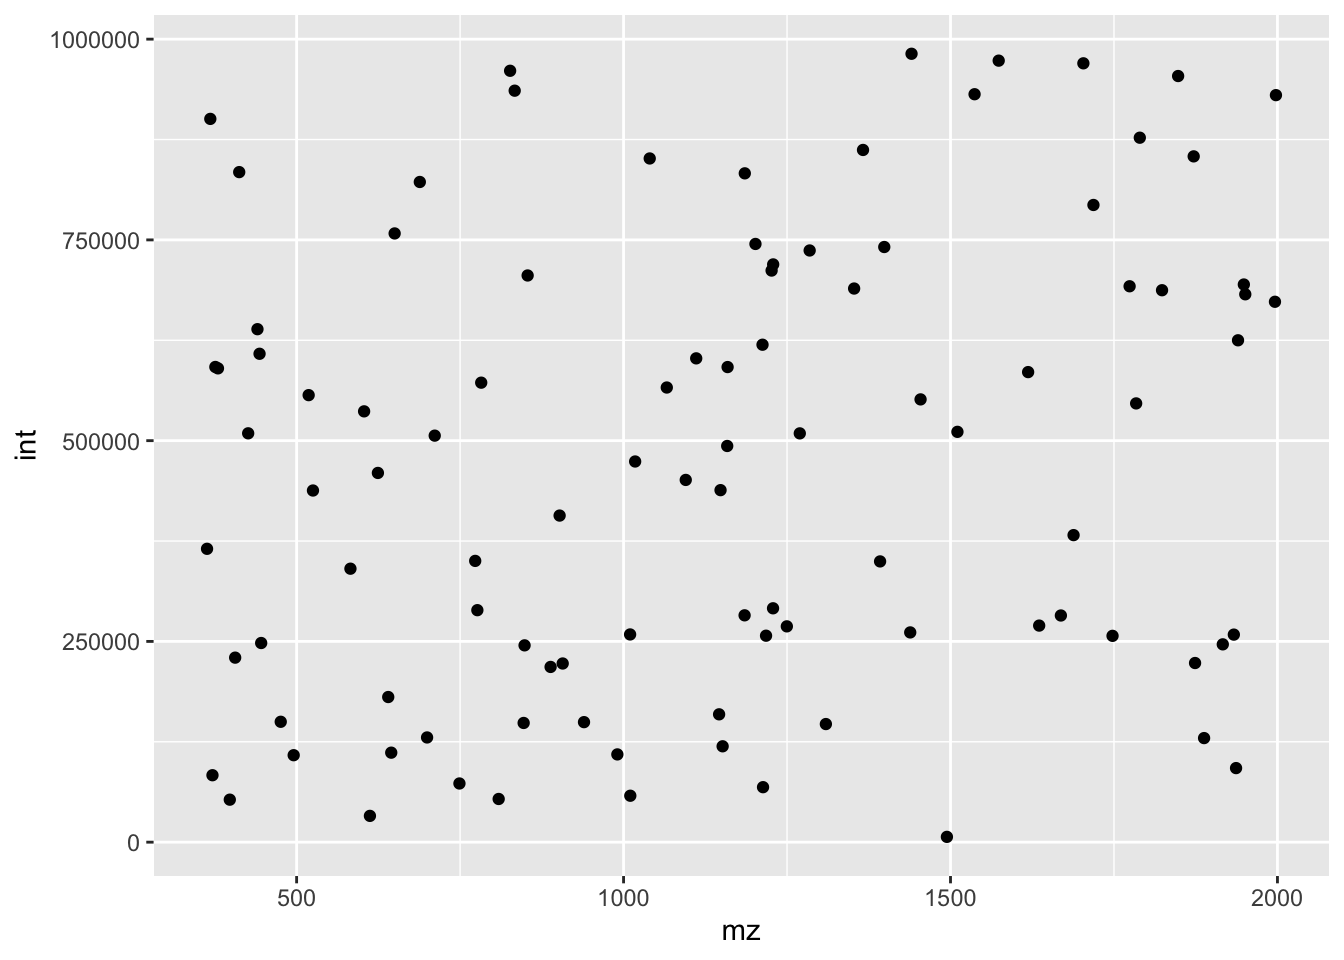
\includegraphics{_main_files/figure-latex/unnamed-chunk-98-1} \end{center}

In data analysis, creating a plot to convey a message or demonstrate a result is a common endpoint. To achieve this, this book utilizes the \texttt{GGPlot2} package, which is part of the \texttt{Tidyverse}. This package complements the data pipelining demonstrated in the previous chapters, making it a perfect choice for creating a wide range of plots, from simple scatter plots to complex heat maps, making it ideal for data visualization.

\hfill\break

\begin{longtable}[]{@{}
  >{\raggedright\arraybackslash}p{(\columnwidth - 2\tabcolsep) * \real{0.3656}}
  >{\raggedright\arraybackslash}p{(\columnwidth - 2\tabcolsep) * \real{0.6344}}@{}}
\toprule\noalign{}
\endhead
\bottomrule\noalign{}
\endlastfoot
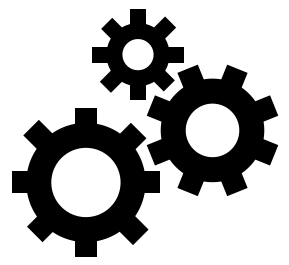
\includegraphics[width=\textwidth,height=0.70833in]{images/03.png} & \begin{minipage}[t]{\linewidth}\raggedright
\textbf{At the end of this chapter you should be able to}

\begin{itemize}
\item
  Understand the need for visualizations.
\item
  Create some simple plots of points, lines and bars.
\item
  Manipulate how a plot looks.
\end{itemize}
\end{minipage} \\
\end{longtable}

\hfill\break

\hypertarget{base-plot}{%
\section{Base: plot}\label{base-plot}}

R comes standard with the fairly basic plotting function \texttt{plot()}. While this function forms the basis for all plotting interactions in R, it can be greatly extended with additional packages. Three such packages widely used are \texttt{lattice}, \texttt{GGplot2}, \texttt{Plotly}. This chapter will dive into \texttt{GGplot2} which is integrated with the tidyverse, and is great for static publication quality plots. The other two will briefly be covered as suitable alternatives.

\begin{Shaded}
\begin{Highlighting}[]
\FunctionTok{plot}\NormalTok{(}\FunctionTok{sample}\NormalTok{(}\DecValTok{1}\SpecialCharTok{:}\DecValTok{20}\NormalTok{),}\FunctionTok{sample}\NormalTok{(}\DecValTok{1}\SpecialCharTok{:}\DecValTok{20}\NormalTok{))}
\end{Highlighting}
\end{Shaded}

\begin{center}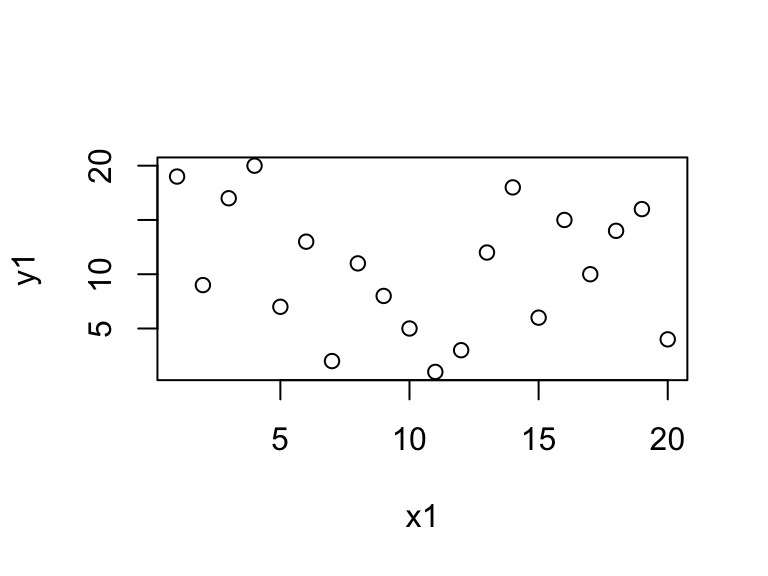
\includegraphics{_main_files/figure-latex/unnamed-chunk-99-1} \end{center}

\begin{Shaded}
\begin{Highlighting}[]
\NormalTok{df }\OtherTok{\textless{}{-}} \FunctionTok{data.frame}\NormalTok{( }\AttributeTok{x1 =} \FunctionTok{sample}\NormalTok{(}\DecValTok{1}\SpecialCharTok{:}\DecValTok{20}\NormalTok{), }\AttributeTok{y1 =} \FunctionTok{sample}\NormalTok{(}\DecValTok{1}\SpecialCharTok{:}\DecValTok{20}\NormalTok{) )}
\NormalTok{df }\SpecialCharTok{\%\textgreater{}\%} \FunctionTok{plot}\NormalTok{()}
\end{Highlighting}
\end{Shaded}

\begin{center}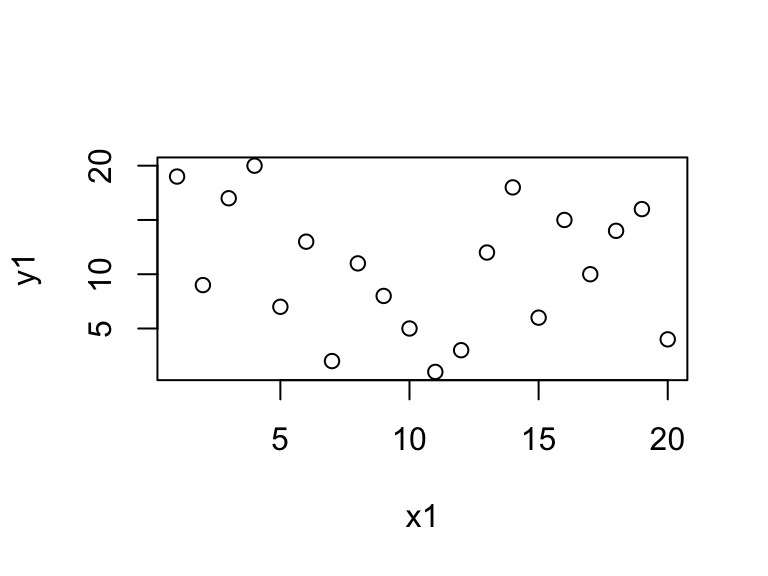
\includegraphics{_main_files/figure-latex/unnamed-chunk-100-1} \end{center}

\hypertarget{ggplot2-1}{%
\section{GGPlot2}\label{ggplot2-1}}

The motivation behind GGplot is based on the grammar of graphics such that

\begin{quote}
\emph{``the idea that you can build every graph from the same few components''}
\end{quote}

Ideally this accomplishes dual goals of allowing you to quickly construct plots for initial analyses and checking for oddities (as explained above) and following the logical process of the plot construction.

\hypertarget{syntax-1}{%
\subsection{Syntax}\label{syntax-1}}

To graph in GGPlot there are a few core embodiments that need to be considered.

\begin{longtable}[]{@{}
  >{\raggedright\arraybackslash}p{(\columnwidth - 4\tabcolsep) * \real{0.2500}}
  >{\raggedright\arraybackslash}p{(\columnwidth - 4\tabcolsep) * \real{0.3750}}
  >{\raggedright\arraybackslash}p{(\columnwidth - 4\tabcolsep) * \real{0.3750}}@{}}
\toprule\noalign{}
\endhead
\bottomrule\noalign{}
\endlastfoot
data & a table of numeric and/or categorical values & data.frame or tibble \\
geom & a geometric object or visual representation, that can be layered & points, lines, bars, boxs, etc. \\
aesthetics & how variables in the data are mapped to visual properties & eg. \emph{x = col\_a, y = col\_b} \\
coordinate & orientation of the data points & eg. \emph{cartesian (x,y), polar} \\
\end{longtable}

\begin{Shaded}
\begin{Highlighting}[]
\CommentTok{\# the basic structure}
\FunctionTok{ggplot}\NormalTok{(data, }\FunctionTok{aes}\NormalTok{(x,y)) }\SpecialCharTok{+} \FunctionTok{geom\_point}\NormalTok{() }\SpecialCharTok{+} \FunctionTok{coord\_cartiesian}\NormalTok{()}

\CommentTok{\# combined with dplyr makes for a readable process}
\NormalTok{data }\SpecialCharTok{\%\textgreater{}\%} \FunctionTok{ggplot}\NormalTok{(}\FunctionTok{aes}\NormalTok{(x,y)) }\SpecialCharTok{+} \FunctionTok{geom\_point}\NormalTok{()}
\end{Highlighting}
\end{Shaded}

In this example the \texttt{ggplot()} function contains the two components, the data table \texttt{data} and mapping function \texttt{aes()}. Since \emph{GGPlot} follows a layered modality, the \texttt{ggplot()} function ``sets'' the canvas and passes the data table \texttt{data} and mapping function \texttt{aes()} to all the functions that follow with the \texttt{+} operator.

\begin{Shaded}
\begin{Highlighting}[]
\FunctionTok{library}\NormalTok{(tidyverse)}
\end{Highlighting}
\end{Shaded}

Lets create some data \ldots{}

\begin{Shaded}
\begin{Highlighting}[]
\FunctionTok{set.seed}\NormalTok{(}\DecValTok{5}\NormalTok{)}
\NormalTok{n\_peaks }\OtherTok{\textless{}{-}} \DecValTok{300}
\NormalTok{tbl\_mz }\OtherTok{\textless{}{-}} \FunctionTok{tibble}\NormalTok{(}
  \AttributeTok{mz =} \FunctionTok{sample}\NormalTok{(}\DecValTok{3500}\SpecialCharTok{:}\DecValTok{20000}\SpecialCharTok{/}\DecValTok{10}\NormalTok{, n\_peaks),}
  \AttributeTok{int =} \FunctionTok{rlnorm}\NormalTok{(}\AttributeTok{meanlog =} \DecValTok{5}\NormalTok{, }\AttributeTok{sdlog =} \DecValTok{2}\NormalTok{, n\_peaks),}
  \AttributeTok{class =} \FunctionTok{sample}\NormalTok{(}\FunctionTok{c}\NormalTok{(}\StringTok{\textquotesingle{}A\textquotesingle{}}\NormalTok{,}\StringTok{\textquotesingle{}B\textquotesingle{}}\NormalTok{,}\StringTok{\textquotesingle{}C\textquotesingle{}}\NormalTok{,}\StringTok{\textquotesingle{}D\textquotesingle{}}\NormalTok{), n\_peaks, }\AttributeTok{replace =} \ConstantTok{TRUE}\NormalTok{) }
\NormalTok{)}
\end{Highlighting}
\end{Shaded}

\hypertarget{basic-data-plotting}{%
\subsection{Basic Data Plotting}\label{basic-data-plotting}}

\hfill\break

\begin{longtable}[]{@{}
  >{\raggedright\arraybackslash}p{(\columnwidth - 2\tabcolsep) * \real{0.3617}}
  >{\raggedright\arraybackslash}p{(\columnwidth - 2\tabcolsep) * \real{0.6383}}@{}}
\toprule\noalign{}
\endhead
\bottomrule\noalign{}
\endlastfoot

\includegraphics[width=\textwidth,height=0.70833in]{images/01.png} & \textbf{Cheat-sheets} \ref{cheat-sheets} \\
\end{longtable}

\hfill\break

\hypertarget{points-and-lines}{%
\subsubsection*{Points and Lines}\label{points-and-lines}}
\addcontentsline{toc}{subsubsection}{Points and Lines}

Points and lines graphing is a simple way of representing data in a two-dimensional space. In this graph, we use points to represent individual data values, and lines to connect them. The x-axis usually represents the \textbf{independent} variable while the y-axis represents the \textbf{dependent} variable - or in other words, what \emph{y} was observed while measuring \emph{x}.

To plot a point, we use an ordered pair of values (x, y) that correspond to the position of the point on the graph. For example, the point (2, 5) would be plotted 2 units to the right on the x-axis and 5 units up on the y-axis.

We can also connect points with lines to show a trend or pattern in the data. These lines can be straight or curved, depending on the nature of the data. A straight line can be drawn to connect two points or to represent a linear relationship between the variables.

\begin{Shaded}
\begin{Highlighting}[]
\NormalTok{p01 }\OtherTok{\textless{}{-}}\NormalTok{ tbl\_mz }\SpecialCharTok{\%\textgreater{}\%} \FunctionTok{ggplot}\NormalTok{(}\FunctionTok{aes}\NormalTok{(mz, int)) }\SpecialCharTok{+} \FunctionTok{geom\_point}\NormalTok{()}
\NormalTok{p02 }\OtherTok{\textless{}{-}}\NormalTok{ tbl\_mz }\SpecialCharTok{\%\textgreater{}\%} \FunctionTok{ggplot}\NormalTok{(}\FunctionTok{aes}\NormalTok{(mz, int)) }\SpecialCharTok{+} \FunctionTok{geom\_line}\NormalTok{()}
\NormalTok{p03 }\OtherTok{\textless{}{-}}\NormalTok{ tbl\_mz }\SpecialCharTok{\%\textgreater{}\%} \FunctionTok{ggplot}\NormalTok{(}\FunctionTok{aes}\NormalTok{(mz, int)) }\SpecialCharTok{+} \FunctionTok{geom\_point}\NormalTok{(}\AttributeTok{color=}\StringTok{\textquotesingle{}red\textquotesingle{}}\NormalTok{) }\SpecialCharTok{+} \FunctionTok{geom\_line}\NormalTok{(}\AttributeTok{color=}\StringTok{\textquotesingle{}black\textquotesingle{}}\NormalTok{)}
\NormalTok{p04 }\OtherTok{\textless{}{-}}\NormalTok{ tbl\_mz }\SpecialCharTok{\%\textgreater{}\%} \FunctionTok{ggplot}\NormalTok{(}\FunctionTok{aes}\NormalTok{(mz, int)) }\SpecialCharTok{+} \FunctionTok{geom\_line}\NormalTok{(}\AttributeTok{color=}\StringTok{\textquotesingle{}black\textquotesingle{}}\NormalTok{) }\SpecialCharTok{+} \FunctionTok{geom\_point}\NormalTok{(}\AttributeTok{color=}\StringTok{\textquotesingle{}red\textquotesingle{}}\NormalTok{)}
\end{Highlighting}
\end{Shaded}

It's important to take note of the difference between plots \emph{p03} and \emph{p04}. While both plots showcase a similar data representation, a closer look reveals a notable difference. Specifically, in the latter plot (\emph{p04}), we can see that the red points appear under the black line. This occurs because the points were layered first, and then the lines were layered over them. This is a crucial distinction to make as it highlights the importance of the order in which layers are applied in the plot.

\begin{center}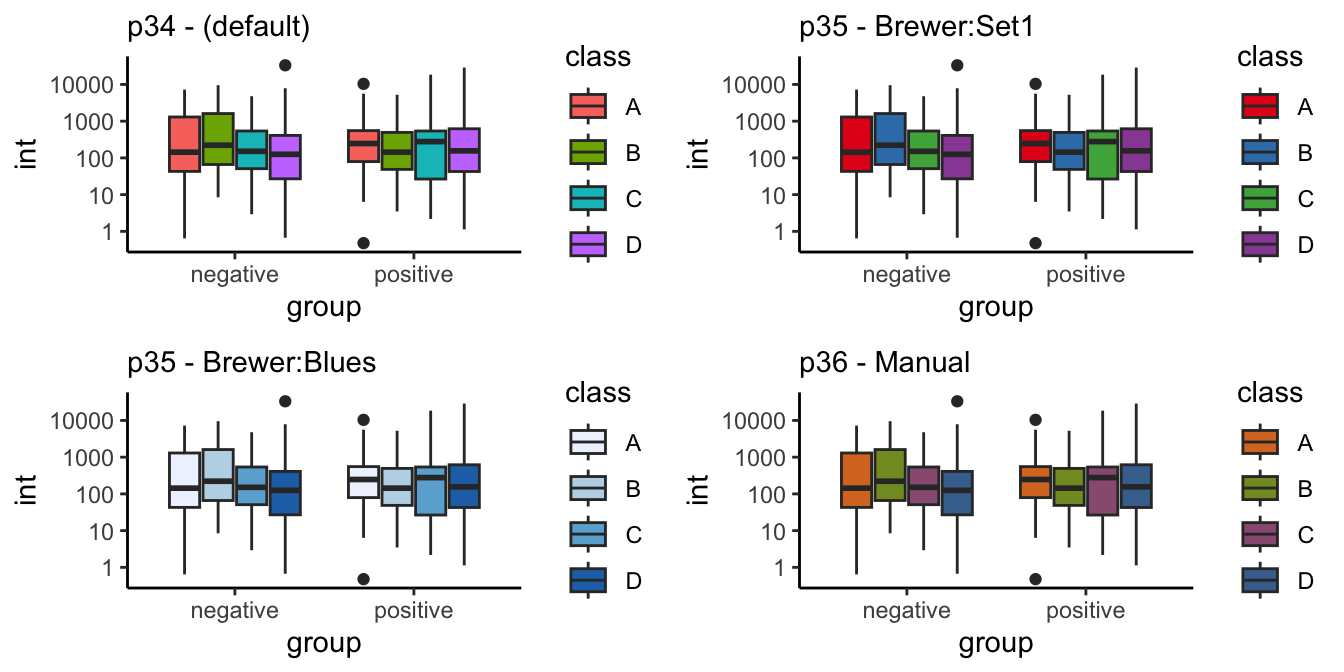
\includegraphics{_main_files/figure-latex/unnamed-chunk-106-1} \end{center}

\hypertarget{segments}{%
\subsubsection*{Segments}\label{segments}}
\addcontentsline{toc}{subsubsection}{Segments}

Line segments are an important concept in geometry and are used in various applications. A line segment is a part of a line that is bounded by two distinct end points. It is also a default representation of centroided mass spectra. In this case the segment will start and end on the same \emph{x} (mz), while the \emph{y} (int) component will end at 0.

\begin{Shaded}
\begin{Highlighting}[]
\NormalTok{p05 }\OtherTok{\textless{}{-}}\NormalTok{ tbl\_mz }\SpecialCharTok{\%\textgreater{}\%} 
  \FunctionTok{ggplot}\NormalTok{(}\FunctionTok{aes}\NormalTok{(mz, int)) }\SpecialCharTok{+} 
  \FunctionTok{geom\_segment}\NormalTok{(}\FunctionTok{aes}\NormalTok{(}\AttributeTok{xend =}\NormalTok{ mz, }\AttributeTok{yend =} \DecValTok{0}\NormalTok{))}
\end{Highlighting}
\end{Shaded}

\begin{center}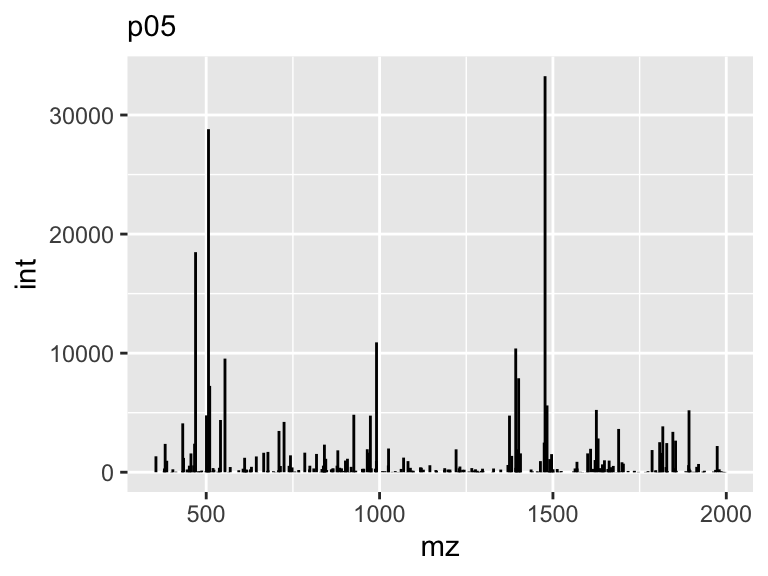
\includegraphics{_main_files/figure-latex/unnamed-chunk-108-1} \end{center}

\hypertarget{bar-chart}{%
\subsubsection*{Bar Chart}\label{bar-chart}}
\addcontentsline{toc}{subsubsection}{Bar Chart}

When it comes to representing categorical data, bar charts are considered to be the most effective visualization tool. Bar charts are simple, yet powerful, and can be used to display data in a clear and concise way. They are easy to read and understand, and are a popular choice among data analysts, researchers, and business professionals. Whether you're trying to visualize sales data, survey results, or demographic information, bar charts are a great option to consider. So, if you're looking for a way to represent categorical data, consider using a bar chart for the most accurate and comprehensive representation.

\begin{Shaded}
\begin{Highlighting}[]
\NormalTok{p06 }\OtherTok{\textless{}{-}}\NormalTok{ tbl\_mz }\SpecialCharTok{\%\textgreater{}\%} 
  \FunctionTok{ggplot}\NormalTok{(}\FunctionTok{aes}\NormalTok{(class)) }\SpecialCharTok{+} 
  \FunctionTok{geom\_bar}\NormalTok{()}
\end{Highlighting}
\end{Shaded}

\begin{center}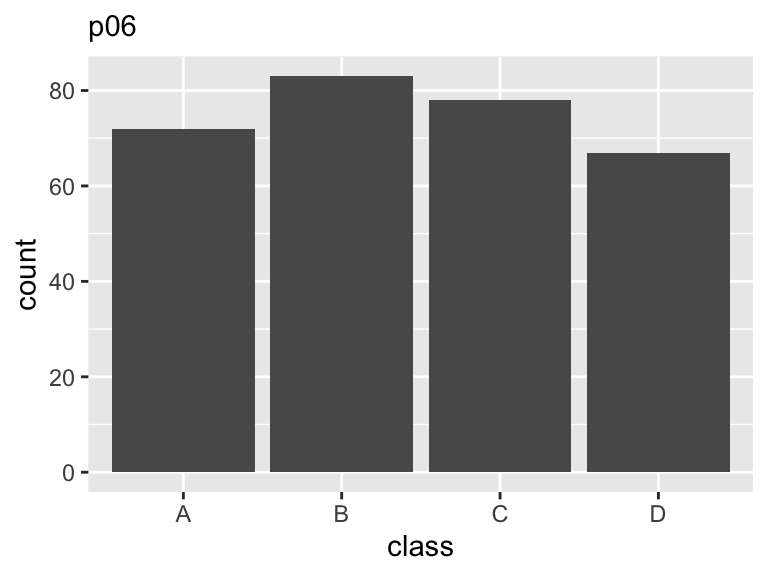
\includegraphics{_main_files/figure-latex/unnamed-chunk-110-1} \end{center}

\hypertarget{pie-chart}{%
\subsubsection*{Pie Chart}\label{pie-chart}}
\addcontentsline{toc}{subsubsection}{Pie Chart}

You maybe considering a pie chart, which is a circular diagram divided into sectors, with each sector representing a proportion of the whole. It is commonly used to display percentages, where the sum of the sectors equals 100\%. There is no specific \texttt{geom} to build a pie-chart with ggplot2. The trick is to build a barplot and use \texttt{coord\_polar()} to make it circular. However, interpreting pie charts can be challenging since humans are not very skilled at reading angles. For instance, it is often difficult to determine which group is the largest and to arrange them by value. As a result, it is advisable to refrain from using pie charts.

\begin{Shaded}
\begin{Highlighting}[]
\NormalTok{p07 }\OtherTok{\textless{}{-}}\NormalTok{ tbl\_mz }\SpecialCharTok{\%\textgreater{}\%} \FunctionTok{ggplot}\NormalTok{(}\FunctionTok{aes}\NormalTok{(class, }\AttributeTok{fill=}\NormalTok{class)) }\SpecialCharTok{+} \FunctionTok{geom\_bar}\NormalTok{()}
\NormalTok{p08 }\OtherTok{\textless{}{-}}\NormalTok{ tbl\_mz }\SpecialCharTok{\%\textgreater{}\%} \FunctionTok{ggplot}\NormalTok{(}\FunctionTok{aes}\NormalTok{(class, }\AttributeTok{fill=}\NormalTok{class)) }\SpecialCharTok{+} \FunctionTok{geom\_bar}\NormalTok{() }\SpecialCharTok{+} \FunctionTok{coord\_flip}\NormalTok{()}
\NormalTok{p09 }\OtherTok{\textless{}{-}}\NormalTok{ tbl\_mz }\SpecialCharTok{\%\textgreater{}\%} \FunctionTok{ggplot}\NormalTok{(}\FunctionTok{aes}\NormalTok{(}\DecValTok{1}\NormalTok{, }\AttributeTok{fill=}\NormalTok{class)) }\SpecialCharTok{+} \FunctionTok{geom\_bar}\NormalTok{(}\AttributeTok{position =} \StringTok{\textquotesingle{}fill\textquotesingle{}}\NormalTok{) }\SpecialCharTok{+} \FunctionTok{coord\_polar}\NormalTok{(}\AttributeTok{theta =} \StringTok{\textquotesingle{}y\textquotesingle{}}\NormalTok{)}
\end{Highlighting}
\end{Shaded}

\begin{center}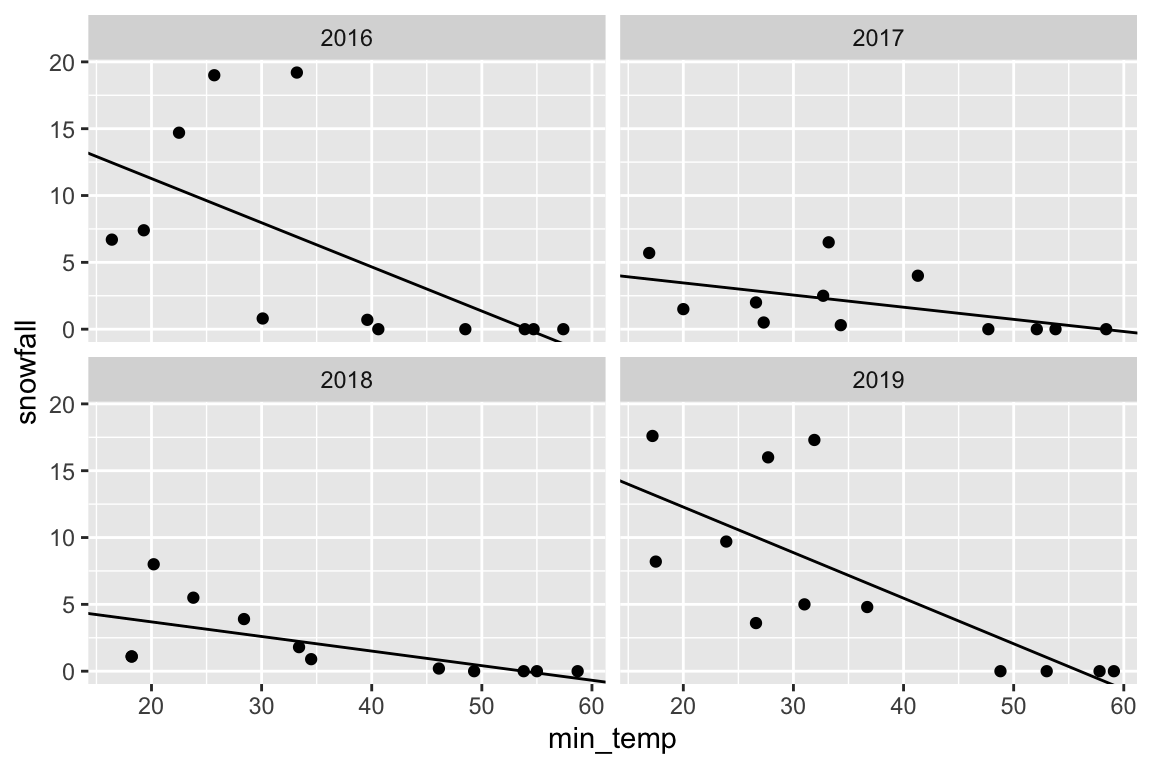
\includegraphics{_main_files/figure-latex/unnamed-chunk-112-1} \end{center}

Note how difficult it is in the pie chart to tell (by eye) that \emph{A} is the smallest.

\hypertarget{data-distributions}{%
\subsection{Data Distributions}\label{data-distributions}}

In statistics, a distribution refers to the way in which a set of data is spread out or dispersed. It describes the pattern of values that a variable can take and how frequently each value occurs. A distribution can be characterized by its shape, center, and spread, and can be represented graphically using tools such as histograms, box plots, and density plots.

\hypertarget{histograms}{%
\subsubsection*{Histograms}\label{histograms}}
\addcontentsline{toc}{subsubsection}{Histograms}

A histogram is a graphical representation of the distribution of a dataset. It is a type of bar chart that displays the frequency of data values falling into specified intervals or ranges of values, known as bins. The x-axis of the histogram represents the bins or intervals, and the y-axis represents the frequency or count of values falling into each bin.

Histograms are widely used to summarize large datasets and identify patterns or trends and to visualize the shape of a distribution, whether it is symmetric or skewed, and whether it has any outliers or gaps in the data. They can also be used to compare the distributions of two or more datasets, by plotting them on the same graph with different colors or patterns.

\begin{Shaded}
\begin{Highlighting}[]
\NormalTok{p10 }\OtherTok{\textless{}{-}}\NormalTok{ tbl\_mz }\SpecialCharTok{\%\textgreater{}\%} 
  \FunctionTok{ggplot}\NormalTok{(}\FunctionTok{aes}\NormalTok{(}\FunctionTok{log10}\NormalTok{(int))) }\SpecialCharTok{+} 
  \FunctionTok{geom\_histogram}\NormalTok{(}\AttributeTok{binwidth =} \DecValTok{1}\NormalTok{)}
\end{Highlighting}
\end{Shaded}

\begin{center}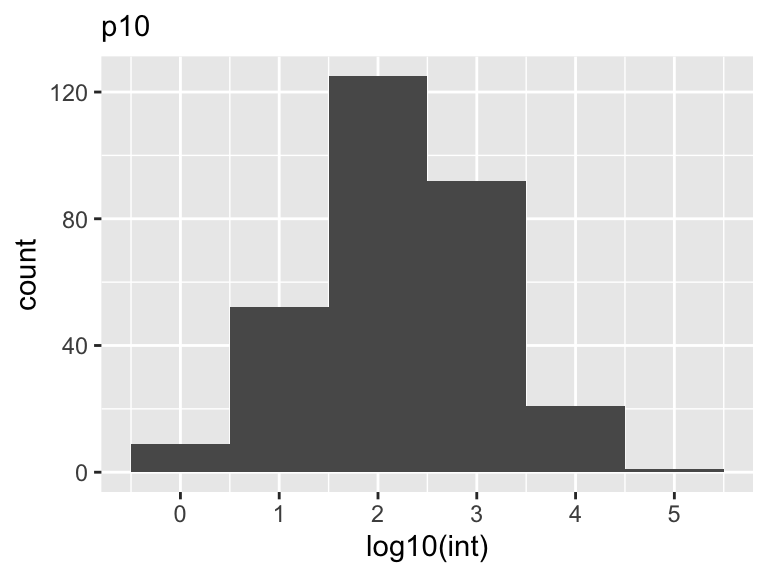
\includegraphics{_main_files/figure-latex/unnamed-chunk-114-1} \end{center}

\hypertarget{density}{%
\subsubsection*{Density}\label{density}}
\addcontentsline{toc}{subsubsection}{Density}

A density plot is a graphical representation of the distribution of a dataset. It is formed by smoothing the data values and representing them as a continuous probability density function. The density plot is a variation of the histogram that provides a smoother representation of the data, eliminating the need for binning. It is particularly useful when the data is continuous and the sample size is large. The density plot can be used to identify the shape of the distribution, the presence of multiple modes, and the presence of outliers. Again, it can also be used to compare the distributions of two or more datasets by overlaying them on the same plot.

\begin{Shaded}
\begin{Highlighting}[]
\NormalTok{p11 }\OtherTok{\textless{}{-}}\NormalTok{ tbl\_mz }\SpecialCharTok{\%\textgreater{}\%} 
  \FunctionTok{ggplot}\NormalTok{(}\FunctionTok{aes}\NormalTok{(}\FunctionTok{log10}\NormalTok{(int))) }\SpecialCharTok{+} 
  \FunctionTok{geom\_density}\NormalTok{()}
\end{Highlighting}
\end{Shaded}

\begin{center}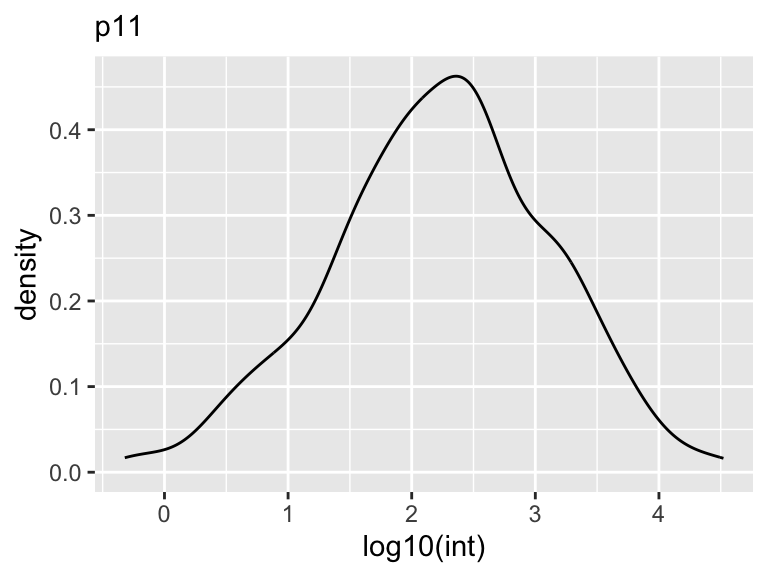
\includegraphics{_main_files/figure-latex/unnamed-chunk-116-1} \end{center}

\hypertarget{box-plot}{%
\subsubsection*{Box-Plot}\label{box-plot}}
\addcontentsline{toc}{subsubsection}{Box-Plot}

One of the most commonly used types of plots in GGplot2 is the box plot. A box plot is used to display the distribution of a continuous variable. It shows the median, interquartile range, and any outliers present in the data.

Box plots are useful in scientific analysis because they allow us to quickly see the distribution of a variable and identify any potential outliers. They are particularly useful when comparing the distribution of a variable across different groups or categories. For example, we may use a box plot to compare the distribution of values across different class levels.

To create a box plot in GGplot2, we use the \texttt{geom\_boxplot()} function. We specify the variable we want to plot on the y-axis and any grouping variables on the x-axis.

\begin{Shaded}
\begin{Highlighting}[]
\NormalTok{p12 }\OtherTok{\textless{}{-}}\NormalTok{ tbl\_mz }\SpecialCharTok{\%\textgreater{}\%} 
  \FunctionTok{ggplot}\NormalTok{(}\FunctionTok{aes}\NormalTok{(class, }\FunctionTok{log10}\NormalTok{(int))) }\SpecialCharTok{+} 
  \FunctionTok{geom\_boxplot}\NormalTok{()}
\end{Highlighting}
\end{Shaded}

\begin{center}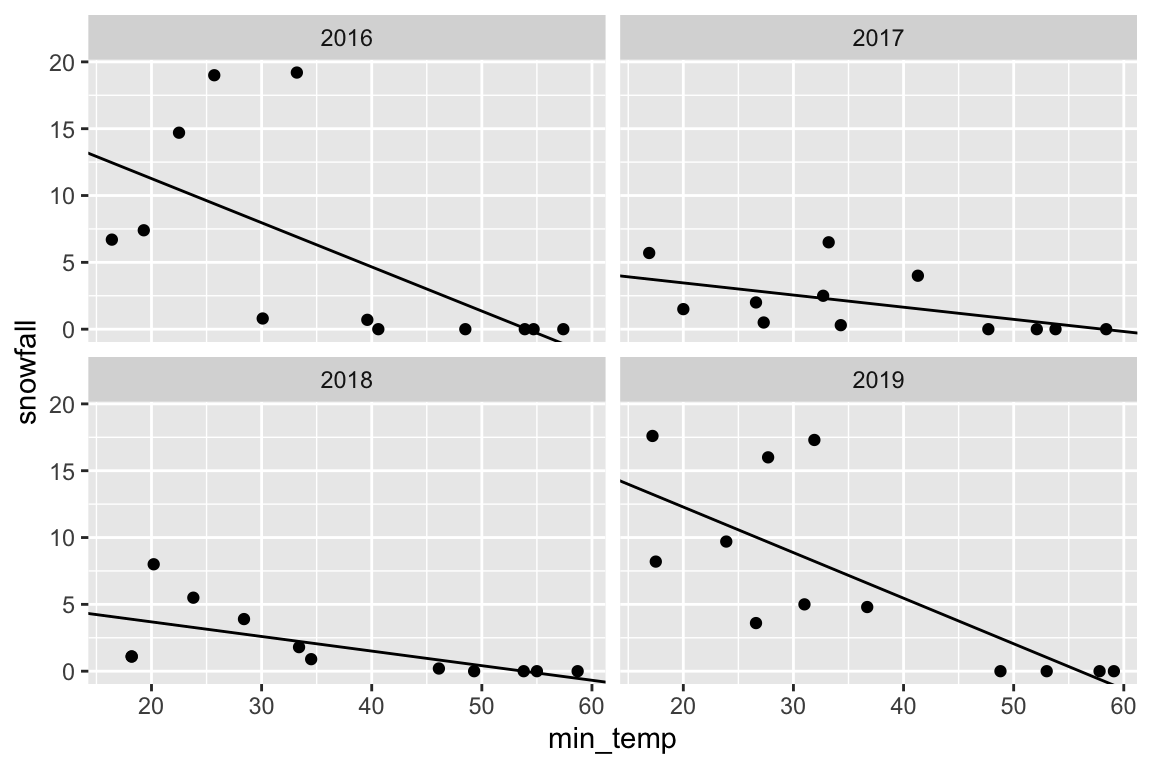
\includegraphics{_main_files/figure-latex/unnamed-chunk-118-1} \end{center}

\hypertarget{extended-syntax}{%
\subsection{Extended Syntax}\label{extended-syntax}}

One way to enhance the functionality of ggplots is by using additional modifiers. These modifiers can help you to create more intricate and detailed visualizations that better represent your data. By tweaking the parameters of your ggplots, you can create visualizations that are more informative, aesthetically pleasing, and tailored to your specific needs. Whether you want to adjust the color scheme, add annotations, or modify the axis labels, additional modifiers can help you to achieve your desired outcome.

\hypertarget{colors}{%
\subsubsection*{Colors}\label{colors}}
\addcontentsline{toc}{subsubsection}{Colors}

We saw a bit how to adjust colors in the previous plots. The two color arguments to consider are \texttt{color}, which modifies the point, line and edge color, and \texttt{fill}, which modifies the internal color of a shape for plots such as \texttt{geom\_bar} and \texttt{geom\_histogram}.

\begin{Shaded}
\begin{Highlighting}[]
\NormalTok{p13 }\OtherTok{\textless{}{-}}\NormalTok{ tbl\_mz }\SpecialCharTok{\%\textgreater{}\%} 
  \FunctionTok{ggplot}\NormalTok{(}\FunctionTok{aes}\NormalTok{(}\FunctionTok{log10}\NormalTok{(int))) }\SpecialCharTok{+} 
  \FunctionTok{geom\_histogram}\NormalTok{(}\AttributeTok{color =} \StringTok{\textquotesingle{}blue\textquotesingle{}}\NormalTok{, }\AttributeTok{fill =} \StringTok{\textquotesingle{}purple\textquotesingle{}}\NormalTok{, }\AttributeTok{binwidth =} \DecValTok{1}\NormalTok{)}

\NormalTok{p14 }\OtherTok{\textless{}{-}}\NormalTok{ tbl\_mz }\SpecialCharTok{\%\textgreater{}\%} 
  \FunctionTok{ggplot}\NormalTok{(}\FunctionTok{aes}\NormalTok{(}\FunctionTok{log10}\NormalTok{(int))) }\SpecialCharTok{+} 
  \FunctionTok{geom\_density}\NormalTok{(}\AttributeTok{color =} \StringTok{\textquotesingle{}red\textquotesingle{}}\NormalTok{, }\AttributeTok{fill =} \StringTok{\textquotesingle{}orange\textquotesingle{}}\NormalTok{)}
\end{Highlighting}
\end{Shaded}

\begin{center}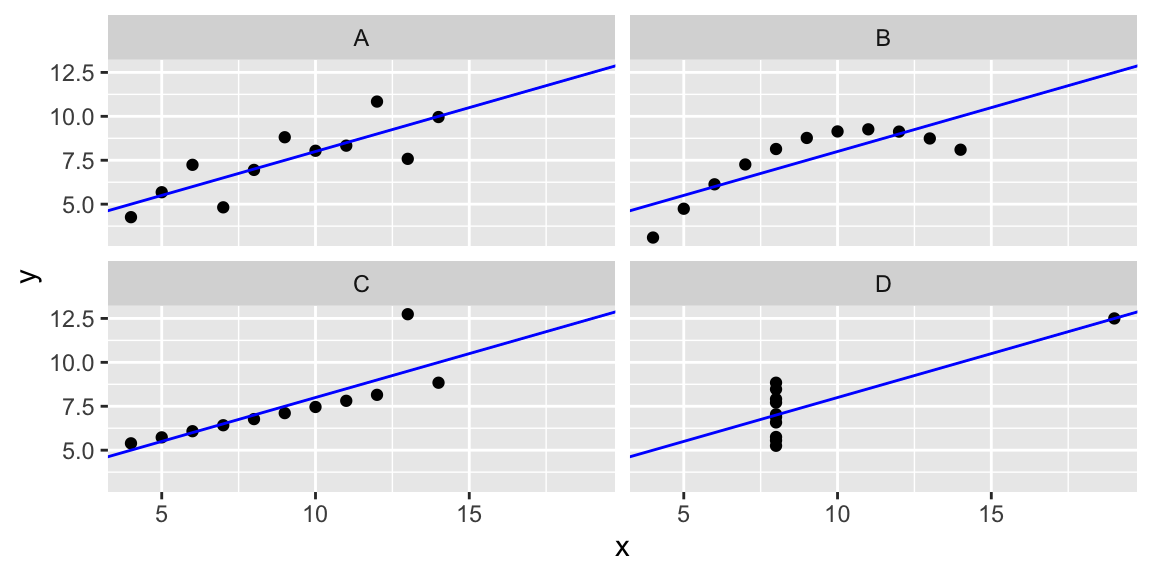
\includegraphics{_main_files/figure-latex/unnamed-chunk-120-1} \end{center}

Colors can also take on a transparency called \texttt{alpha}, which allows one layer to show through when two or more are plotted together.

\begin{Shaded}
\begin{Highlighting}[]
\NormalTok{p15 }\OtherTok{\textless{}{-}}\NormalTok{ tbl\_mz }\SpecialCharTok{\%\textgreater{}\%} 
  \FunctionTok{ggplot}\NormalTok{(}\FunctionTok{aes}\NormalTok{(}\FunctionTok{log10}\NormalTok{(int))) }\SpecialCharTok{+} 
  \FunctionTok{geom\_density}\NormalTok{(}\FunctionTok{aes}\NormalTok{(}\AttributeTok{fill =}\NormalTok{ class))}

\NormalTok{p16 }\OtherTok{\textless{}{-}}\NormalTok{ tbl\_mz }\SpecialCharTok{\%\textgreater{}\%} 
  \FunctionTok{ggplot}\NormalTok{(}\FunctionTok{aes}\NormalTok{(}\FunctionTok{log10}\NormalTok{(int))) }\SpecialCharTok{+} 
  \FunctionTok{geom\_density}\NormalTok{(}\FunctionTok{aes}\NormalTok{(}\AttributeTok{fill =}\NormalTok{ class), }\AttributeTok{alpha =}\NormalTok{ .}\DecValTok{25}\NormalTok{)}
\end{Highlighting}
\end{Shaded}

\begin{center}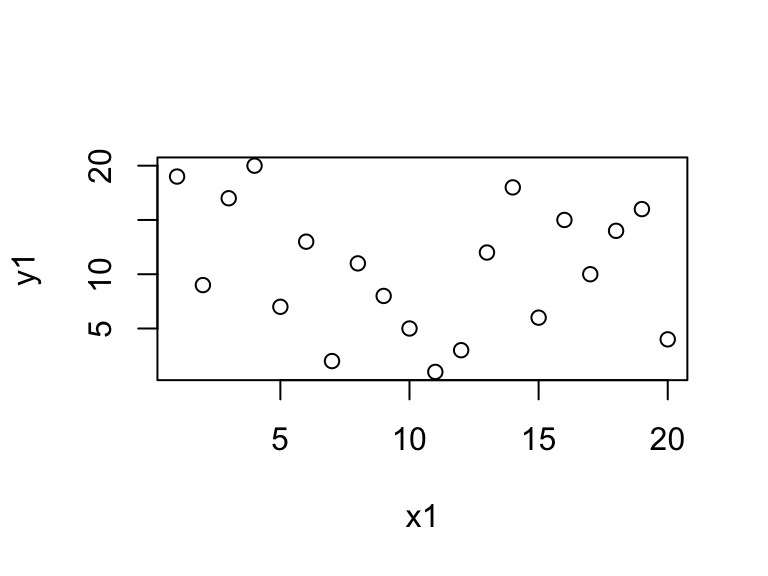
\includegraphics{_main_files/figure-latex/unnamed-chunk-122-1} \end{center}

\hypertarget{scales}{%
\subsubsection*{Scales}\label{scales}}
\addcontentsline{toc}{subsubsection}{Scales}

GGplot2 is a popular data visualization package in R that allows users to create stunning and insightful visualizations. One of the key features of GGplot2 is its ability to handle scales, which are critical for displaying data accurately and effectively. In this document, we will explore how to use scales in GGplot2, specifically for log10 and manual scales.

\hypertarget{log10-scale}{%
\paragraph*{Log10 Scale}\label{log10-scale}}
\addcontentsline{toc}{paragraph}{Log10 Scale}

Logarithmic scales are useful when the data spans several orders of magnitude. GGplot2 makes it easy to create log10 scales using the \texttt{scale\_y\_log10()} and \texttt{scale\_x\_log10()} functions.

Using the same examples from above, yet instead of applying the \texttt{log10()} function directly to the variable, we can apply it to the scale instead.

\begin{Shaded}
\begin{Highlighting}[]
\NormalTok{p17 }\OtherTok{\textless{}{-}}\NormalTok{ tbl\_mz }\SpecialCharTok{\%\textgreater{}\%} 
  \FunctionTok{ggplot}\NormalTok{(}\FunctionTok{aes}\NormalTok{(int)) }\SpecialCharTok{+} 
  \FunctionTok{geom\_histogram}\NormalTok{(}\FunctionTok{aes}\NormalTok{(}\AttributeTok{fill =}\NormalTok{ class), }\AttributeTok{position =} \StringTok{\textquotesingle{}identity\textquotesingle{}}\NormalTok{, }\AttributeTok{alpha =}\NormalTok{ .}\DecValTok{5}\NormalTok{, }\AttributeTok{binwidth =} \DecValTok{1}\NormalTok{) }\SpecialCharTok{+}
  \FunctionTok{scale\_x\_log10}\NormalTok{()}

\NormalTok{p18 }\OtherTok{\textless{}{-}}\NormalTok{ tbl\_mz }\SpecialCharTok{\%\textgreater{}\%} 
  \FunctionTok{ggplot}\NormalTok{(}\FunctionTok{aes}\NormalTok{(int)) }\SpecialCharTok{+} 
  \FunctionTok{geom\_density}\NormalTok{(}\FunctionTok{aes}\NormalTok{(}\AttributeTok{fill =}\NormalTok{ class), }\AttributeTok{alpha =}\NormalTok{ .}\DecValTok{25}\NormalTok{) }\SpecialCharTok{+}
  \FunctionTok{scale\_x\_log10}\NormalTok{()}
\end{Highlighting}
\end{Shaded}

\begin{center}\includegraphics{_main_files/figure-latex/unnamed-chunk-124-1} \end{center}

This results in a plot where the y-axis is scaled logarithmically, making it easier to see the differences between the different car classes. Note, that when we specified the \texttt{binwidth\ =\ 1} in the \texttt{geom\_histogram()}, GGplot2 applied that to the log10 space specified from the \texttt{scale\_x\_log10()}.

\hypertarget{manual-scales}{%
\paragraph*{Manual Scales}\label{manual-scales}}
\addcontentsline{toc}{paragraph}{Manual Scales}

Sometimes, we may want to manually define the scale for our plots. For example, we may want to create a plot where the y-axis only shows values between 0 and 10. We can do this using the \texttt{scale\_y\_continuous()} function in GGplot2.

Here is an example of how to use the \texttt{scale\_y\_continuous()} function to manually define the y-axis scale:

\begin{Shaded}
\begin{Highlighting}[]
\NormalTok{p19 }\OtherTok{\textless{}{-}}\NormalTok{ tbl\_mz }\SpecialCharTok{\%\textgreater{}\%} 
  \FunctionTok{ggplot}\NormalTok{(}\FunctionTok{aes}\NormalTok{(mz, int)) }\SpecialCharTok{+} 
  \FunctionTok{geom\_segment}\NormalTok{(}\FunctionTok{aes}\NormalTok{(}\AttributeTok{xend =}\NormalTok{ mz, }\AttributeTok{yend =} \DecValTok{0}\NormalTok{)) }\SpecialCharTok{+}
  \FunctionTok{scale\_y\_continuous}\NormalTok{(}\AttributeTok{n.breaks =} \DecValTok{13}\NormalTok{) }\SpecialCharTok{+}
  \FunctionTok{scale\_x\_continuous}\NormalTok{(}\AttributeTok{n.breaks =} \DecValTok{5}\NormalTok{, }\AttributeTok{limits =} \FunctionTok{c}\NormalTok{(}\DecValTok{500}\NormalTok{,}\DecValTok{1500}\NormalTok{))}
\end{Highlighting}
\end{Shaded}

\begin{center}\includegraphics{_main_files/figure-latex/unnamed-chunk-126-1} \end{center}

In this example, we added a manual scale to both the x- and y-axis using the \texttt{scale\_x\_continuous()} and \texttt{scale\_y\_continuous()} functions, respectively, and specifying the number of breaks \texttt{n.breaks\ =} and the limits \texttt{limits\ =}.

\hypertarget{faceting}{%
\paragraph*{Faceting}\label{faceting}}
\addcontentsline{toc}{paragraph}{Faceting}

Faceting is a powerful feature in ggplot2 that allows us to split a single plot into multiple small plots based on a categorical variable. It enables us to visualize complex data patterns and relationships in a more understandable way. There are two types of faceting in ggplot2: facet\_wrap and facet\_grid.

\hypertarget{facet_wrap}{%
\subparagraph*{facet\_wrap}\label{facet_wrap}}
\addcontentsline{toc}{subparagraph}{facet\_wrap}

\texttt{facet\_wrap} creates a grid of plots by wrapping the facets from left-to-right and top-to-bottom in the plot. Each facet is displayed in a separate panel, and the panels are arranged in rows and columns based on the levels of the specified categorical variable.

\begin{Shaded}
\begin{Highlighting}[]
\NormalTok{p20 }\OtherTok{\textless{}{-}}\NormalTok{ p17 }\SpecialCharTok{+} \FunctionTok{facet\_wrap}\NormalTok{(. }\SpecialCharTok{\textasciitilde{}}\NormalTok{ class)}

\NormalTok{p21 }\OtherTok{\textless{}{-}}\NormalTok{ p17 }\SpecialCharTok{+} \FunctionTok{facet\_wrap}\NormalTok{(. }\SpecialCharTok{\textasciitilde{}}\NormalTok{ class, }\AttributeTok{scales =} \StringTok{\textquotesingle{}free\textquotesingle{}}\NormalTok{)}
\end{Highlighting}
\end{Shaded}

\begin{center}\includegraphics{_main_files/figure-latex/unnamed-chunk-128-1} \end{center}

In this example, we are reused ggplot object \texttt{p17} and created two additional plots. The \texttt{facet\_wrap} function is used to split the plot into multiple panels based on the categorical variable \texttt{class} using the tilde \texttt{.\ \textasciitilde{}\ class}. In this case, the dot \texttt{.} prior to the tilde \texttt{\textasciitilde{}} tells ggplot to consider only a single variable, \texttt{class} as we had defined it. You can think of the tilde as a type of function \texttt{this\ \textquotesingle{}by\textquotesingle{}\ that} or \texttt{y\ \textasciitilde{}\ x}. This becomes more important in the \texttt{facet\_grid()} function. Notice in the \texttt{p21} plot we set the scales \texttt{free}, allowing each facet to dictate \texttt{x} and \texttt{y} plot scales.

\hypertarget{facet_grid}{%
\subparagraph*{facet\_grid}\label{facet_grid}}
\addcontentsline{toc}{subparagraph}{facet\_grid}

\texttt{facet\_grid} creates a grid of plots by specifying one or more categorical variables that define the rows and columns of the grid. It allows us to create more complex faceted plots than \texttt{facet\_wrap}. In this example we will randomly add a new varaible called \texttt{group} that will allow us to create the \texttt{y} direction of the facet.

\begin{Shaded}
\begin{Highlighting}[]
\NormalTok{tbl\_new }\OtherTok{\textless{}{-}}\NormalTok{ tbl\_mz }\SpecialCharTok{\%\textgreater{}\%}
  \FunctionTok{mutate}\NormalTok{(}\AttributeTok{group =} \FunctionTok{sample}\NormalTok{(}\FunctionTok{c}\NormalTok{(}\StringTok{\textquotesingle{}positive\textquotesingle{}}\NormalTok{, }\StringTok{\textquotesingle{}negative\textquotesingle{}}\NormalTok{), n\_peaks, }\AttributeTok{replace =} \ConstantTok{TRUE}\NormalTok{))}

\NormalTok{p22 }\OtherTok{\textless{}{-}}\NormalTok{ tbl\_new }\SpecialCharTok{\%\textgreater{}\%} 
  \FunctionTok{ggplot}\NormalTok{(}\FunctionTok{aes}\NormalTok{(int)) }\SpecialCharTok{+} 
  \FunctionTok{geom\_histogram}\NormalTok{(}\AttributeTok{binwidth =} \DecValTok{1}\NormalTok{) }\SpecialCharTok{+}
  \FunctionTok{scale\_x\_log10}\NormalTok{() }\SpecialCharTok{+}
  \FunctionTok{facet\_grid}\NormalTok{(group }\SpecialCharTok{\textasciitilde{}}\NormalTok{ class)}
\end{Highlighting}
\end{Shaded}

\begin{center}\includegraphics{_main_files/figure-latex/unnamed-chunk-130-1} \end{center}

To illistrate the difference between \texttt{facet\_wrap()} and \texttt{facet\_grid()} consider what happens when a set of data is missing. Note in \texttt{p24} it is not immediately intuitive in \texttt{facet\_wrap()} that \texttt{c-negative} is missing, where as in \texttt{facet\_grid()}, the layout highlights this realization.

\begin{Shaded}
\begin{Highlighting}[]
\NormalTok{tbl\_new }\OtherTok{\textless{}{-}}\NormalTok{ tbl\_mz }\SpecialCharTok{\%\textgreater{}\%}
  \FunctionTok{mutate}\NormalTok{(}\AttributeTok{group =} \FunctionTok{sample}\NormalTok{(}\FunctionTok{c}\NormalTok{(}\StringTok{\textquotesingle{}positive\textquotesingle{}}\NormalTok{, }\StringTok{\textquotesingle{}negative\textquotesingle{}}\NormalTok{), n\_peaks, }\AttributeTok{replace =} \ConstantTok{TRUE}\NormalTok{))}

\NormalTok{w }\OtherTok{\textless{}{-}} \FunctionTok{which}\NormalTok{(tbl\_new}\SpecialCharTok{$}\NormalTok{class }\SpecialCharTok{==} \StringTok{\textquotesingle{}C\textquotesingle{}} \SpecialCharTok{\&}\NormalTok{ tbl\_new}\SpecialCharTok{$}\NormalTok{group }\SpecialCharTok{==} \StringTok{\textquotesingle{}negative\textquotesingle{}}\NormalTok{)}

\NormalTok{p23 }\OtherTok{\textless{}{-}}\NormalTok{ tbl\_new[}\SpecialCharTok{{-}}\NormalTok{w, ] }\SpecialCharTok{\%\textgreater{}\%} 
  \FunctionTok{ggplot}\NormalTok{(}\FunctionTok{aes}\NormalTok{(int)) }\SpecialCharTok{+} 
  \FunctionTok{geom\_histogram}\NormalTok{(}\AttributeTok{binwidth =} \DecValTok{1}\NormalTok{) }\SpecialCharTok{+}
  \FunctionTok{scale\_x\_log10}\NormalTok{()}

\NormalTok{p24 }\OtherTok{\textless{}{-}}\NormalTok{ p23 }\SpecialCharTok{+} \FunctionTok{facet\_wrap}\NormalTok{(group }\SpecialCharTok{\textasciitilde{}}\NormalTok{ class)}
\NormalTok{p25 }\OtherTok{\textless{}{-}}\NormalTok{ p23 }\SpecialCharTok{+} \FunctionTok{facet\_grid}\NormalTok{(group }\SpecialCharTok{\textasciitilde{}}\NormalTok{ class)}
\end{Highlighting}
\end{Shaded}

\begin{center}\includegraphics{_main_files/figure-latex/unnamed-chunk-132-1} \end{center}

\hypertarget{labels}{%
\subsubsection*{Labels}\label{labels}}
\addcontentsline{toc}{subsubsection}{Labels}

\hypertarget{annotations}{%
\subsubsection*{Annotations}\label{annotations}}
\addcontentsline{toc}{subsubsection}{Annotations}

\hypertarget{style}{%
\subsubsection*{Style}\label{style}}
\addcontentsline{toc}{subsubsection}{Style}

Creating a plotting style can help you to quickly improve the appearance of your plots and make them more consistent with your brand. When working with data visualization, it's important to keep in mind that the appearance of your plots can significantly impact the way your audience interprets your data. GGplot2 themes and colors offer an easy way to create professional-looking visualizations that will make your data stand out.

\hypertarget{themes}{%
\paragraph*{Themes}\label{themes}}
\addcontentsline{toc}{paragraph}{Themes}

To apply a theme to your plot, you simply need to call the \texttt{theme()} function and specify the name of the theme you want to use. Some of the most popular themes include:

\begin{itemize}
\tightlist
\item
  \texttt{theme\_gray()}: A simple, gray background with white gridlines.
\item
  \texttt{theme\_dark()}: A simple, gray background with white gridlines.
\item
  \texttt{theme\_classic()}: A classic black and white theme with no gridlines.
\item
  \texttt{theme\_minimal()}: A minimalistic theme with no background or gridlines.
\item
  \texttt{theme\_bw()}: A black and white theme with gray gridlines.
\end{itemize}

You can also create your own custom themes by modifying various theme elements. For example, you can change the background color, font, and size of the plot elements. To do this, you can use the \texttt{element\_*()} functions. For example, the \texttt{element\_text()} function allows you to modify the font size, color, and family of your text.

Another great feature of GGplot2 themes is that they allow you to maintain consistency across multiple visualizations. If you're creating a series of plots, applying the same theme to each one will give your work a more polished and professional look.

\begin{Shaded}
\begin{Highlighting}[]
\NormalTok{p28 }\OtherTok{\textless{}{-}}\NormalTok{ p12 }\SpecialCharTok{+} \FunctionTok{theme\_gray}\NormalTok{() }\CommentTok{\# default}
\NormalTok{p29 }\OtherTok{\textless{}{-}}\NormalTok{ p12 }\SpecialCharTok{+} \FunctionTok{theme\_dark}\NormalTok{()}
\NormalTok{p30 }\OtherTok{\textless{}{-}}\NormalTok{ p12 }\SpecialCharTok{+} \FunctionTok{theme\_light}\NormalTok{()}
\NormalTok{p31 }\OtherTok{\textless{}{-}}\NormalTok{ p12 }\SpecialCharTok{+} \FunctionTok{theme\_classic}\NormalTok{()}
\NormalTok{p32 }\OtherTok{\textless{}{-}}\NormalTok{ p12 }\SpecialCharTok{+} \FunctionTok{theme\_minimal}\NormalTok{()}
\NormalTok{p33 }\OtherTok{\textless{}{-}}\NormalTok{ p12 }\SpecialCharTok{+} \FunctionTok{theme\_bw}\NormalTok{()}
\end{Highlighting}
\end{Shaded}

\begin{center}\includegraphics{_main_files/figure-latex/unnamed-chunk-135-1} \end{center}

\hypertarget{colors-1}{%
\paragraph*{Colors}\label{colors-1}}
\addcontentsline{toc}{paragraph}{Colors}

In addition to applying a theme to your layout, you can should also consider the color scheme. GGplot2 is a powerful data visualization package in R that allows users to create beautiful and informative graphs. The package is highly customizable, and one of its most important features is the ability to customize colors using Brewer and manual color scales.

\hypertarget{brewer-color-scales}{%
\subparagraph*{Brewer Color Scales}\label{brewer-color-scales}}
\addcontentsline{toc}{subparagraph}{Brewer Color Scales}

The Brewer color scales in GGplot2 are color palettes that have been specifically designed to be distinguishable by people with color vision deficiencies. These color scales are useful when creating visualizations where color is used to convey information.

The Brewer palettes are particularly useful because they are carefully curated to ensure that the colors are distinguishable from one another, even for individuals with color vision deficiencies. This makes them a great option for creating informative data visualizations.

To use Brewer color scales in GGplot2, you can simply specify the name of the color scale as an argument to the \texttt{scale\_color\_brewer()} or \texttt{scale\_fill\_brewer()} functions. Other popular Brewer color scales include Blues, Greens, Oranges, and Purples. By using these scales, you can create beautiful visualizations that are both aesthetically pleasing and informative.

\hypertarget{manual-color-scales}{%
\subparagraph*{Manual Color Scales}\label{manual-color-scales}}
\addcontentsline{toc}{subparagraph}{Manual Color Scales}

In addition to the Brewer color scales, GGplot2 also allows users to specify custom color scales using the \texttt{scale\_color\_manual()} or \texttt{scale\_fill\_manual()} functions. These functions take a vector of colors as an argument, which can be specified using names, hex codes, or RGB values.

Manual color scales are particularly useful when you want to use specific colors that are not included in the Brewer palettes. For example, if you are creating a visualization for a company and you want to use the company's brand colors, you can specify the colors using a manual color scale.

\begin{Shaded}
\begin{Highlighting}[]
\NormalTok{p34 }\OtherTok{\textless{}{-}}\NormalTok{ p31}
\NormalTok{p35 }\OtherTok{\textless{}{-}}\NormalTok{ p31 }\SpecialCharTok{+} \FunctionTok{scale\_fill\_brewer}\NormalTok{(}\AttributeTok{palette =} \StringTok{\textquotesingle{}Set1\textquotesingle{}}\NormalTok{)}
\NormalTok{p36 }\OtherTok{\textless{}{-}}\NormalTok{ p31 }\SpecialCharTok{+} \FunctionTok{scale\_fill\_brewer}\NormalTok{(}\AttributeTok{palette =} \StringTok{\textquotesingle{}Blues\textquotesingle{}}\NormalTok{)}
\NormalTok{p37 }\OtherTok{\textless{}{-}}\NormalTok{ p31 }\SpecialCharTok{+} \FunctionTok{scale\_fill\_manual}\NormalTok{(}\AttributeTok{values =} \FunctionTok{c}\NormalTok{(}\StringTok{"\#d97828"}\NormalTok{, }\StringTok{"\#83992a"}\NormalTok{, }\StringTok{"\#995d81"}\NormalTok{,}\StringTok{"\#44709d"}\NormalTok{))}
\end{Highlighting}
\end{Shaded}

\begin{center}\includegraphics{_main_files/figure-latex/unnamed-chunk-138-1} \end{center}

\hypertarget{package-ggrepel}{%
\subsubsection*{Package ggrepel}\label{package-ggrepel}}
\addcontentsline{toc}{subsubsection}{Package ggrepel}

\hypertarget{alternatives-1}{%
\section{Alternatives}\label{alternatives-1}}

\hypertarget{lattice}{%
\subsection*{lattice}\label{lattice}}
\addcontentsline{toc}{subsection}{lattice}

The Lattice package is an R package that is used for plotting graphs, and is based on the grid graphics system. The package provides a high-level interface to grid graphics, which makes it easy to create complex visualizations with an emphasis on multivariate data. It is designed to meet most typical graphics needs with minimal tuning, but can also be easily extended to handle most nonstandard requirements.

Trellis Graphics, originally developed for S and S-PLUS at the Bell Labs, is a framework for data visualization developed by \emph{R. A. Becker, W. S. Cleveland, et al, extending ideas presented in Cleveland's 1993 book Visualizing Data}. The Lattice API is based on the original design in S, but extends it in many ways.

Various types of lattice plots available for data visualization. Among the different types of plots, \textbf{univariate} plots stand out as they utilize only a single variable for plotting. The different options available for univariate plots include bar plots, box-and-whisker plots, kernel density estimates, dot plots, histograms, quantile plots, and one-dimensional scatter plots. \textbf{Bivariate} plots involve plotting two variables against each other. Examples of bivariate plots include scatterplots and quantile plots. These types of plots are useful in analyzing the relationship between two variables and can provide valuable insights into the data. \textbf{Trivariate} plots, as the name implies, involve plotting three variables and provide a more complex visualization of the data. Options for trivariate plots include level plots, contour plots, three-dimensional scatter plots, and three-dimensional surface plots. These types of plots can be particularly helpful in analyzing complex data sets and identifying patterns in the data that may not be immediately apparent.

\begin{Shaded}
\begin{Highlighting}[]
\FunctionTok{library}\NormalTok{(lattice)}

\NormalTok{p51 }\OtherTok{\textless{}{-}} \FunctionTok{xyplot}\NormalTok{(int }\SpecialCharTok{\textasciitilde{}}\NormalTok{ mz, }\AttributeTok{data =}\NormalTok{ tbl\_mz, }\AttributeTok{main =} \StringTok{"Scatter Plot"}\NormalTok{)}
\NormalTok{p52 }\OtherTok{\textless{}{-}} \FunctionTok{xyplot}\NormalTok{(int }\SpecialCharTok{\textasciitilde{}}\NormalTok{ mz, }\AttributeTok{data =}\NormalTok{ tbl\_mz, }\AttributeTok{type=}\StringTok{\textquotesingle{}a\textquotesingle{}}\NormalTok{, }\AttributeTok{main =} \StringTok{"Line Plot"}\NormalTok{)}
\NormalTok{p53 }\OtherTok{\textless{}{-}} \FunctionTok{histogram}\NormalTok{(}\SpecialCharTok{\textasciitilde{}} \FunctionTok{log10}\NormalTok{(int) }\SpecialCharTok{|}\NormalTok{ class, }\AttributeTok{data =}\NormalTok{ tbl\_mz, }\AttributeTok{main =} \StringTok{"Histogram"}\NormalTok{)}
\NormalTok{p54 }\OtherTok{\textless{}{-}} \FunctionTok{densityplot}\NormalTok{(}\SpecialCharTok{\textasciitilde{}} \FunctionTok{log10}\NormalTok{(int) }\SpecialCharTok{|}\NormalTok{ class, }\AttributeTok{data =}\NormalTok{ tbl\_mz, }\AttributeTok{main =} \StringTok{"Density Plot"}\NormalTok{)}
\end{Highlighting}
\end{Shaded}

\begin{center}\includegraphics{_main_files/figure-latex/unnamed-chunk-140-1} \end{center}

\hypertarget{plotly}{%
\subsection*{plotly}\label{plotly}}
\addcontentsline{toc}{subsection}{plotly}

Plotly is an open-source data visualization library that allows you to create interactive visualizations in R \href{https://plotly.com/r/}{plotly.com/r/}. It offers a wide range of graphs and charts, including line plots, scatter plots, area charts, bar charts, error bars, box plots, histograms, heatmaps, subplots, plots with multiple-axes, 3D plots, and more. The package is built on top of \textbf{htmlwidgets}, which means that you can easily embed your visualizations in web applications or other HTML documents.

Plotly also nativity supports many data science languages such as R, Python, Julia, Java-script, MATLAB and F\#.

\begin{Shaded}
\begin{Highlighting}[]
\FunctionTok{library}\NormalTok{(plotly)}
\end{Highlighting}
\end{Shaded}

\begin{Shaded}
\begin{Highlighting}[]
\FunctionTok{plot\_ly}\NormalTok{(tbl\_mz, }\AttributeTok{x =} \SpecialCharTok{\textasciitilde{}}\NormalTok{mz, }\AttributeTok{y =} \SpecialCharTok{\textasciitilde{}}\NormalTok{int, }\AttributeTok{color =} \SpecialCharTok{\textasciitilde{}}\NormalTok{class,}
        \AttributeTok{mode =} \StringTok{"markers"}\NormalTok{, }\AttributeTok{type =} \StringTok{"scatter"}\NormalTok{) }\SpecialCharTok{\%\textgreater{}\%} 
  \FunctionTok{layout}\NormalTok{(}\AttributeTok{title =} \StringTok{\textquotesingle{}Scatter Plot\textquotesingle{}}\NormalTok{)}
\end{Highlighting}
\end{Shaded}

\hypertarget{exercises-5}{%
\section*{Exercises}\label{exercises-5}}
\addcontentsline{toc}{section}{Exercises}

\begin{longtable}[]{@{}
  >{\raggedright\arraybackslash}p{(\columnwidth - 2\tabcolsep) * \real{0.3091}}
  >{\raggedright\arraybackslash}p{(\columnwidth - 2\tabcolsep) * \real{0.6909}}@{}}
\toprule\noalign{}
\endhead
\bottomrule\noalign{}
\endlastfoot
\includegraphics[width=\textwidth,height=0.70833in]{images/07.png} & \begin{minipage}[t]{\linewidth}\raggedright
\begin{itemize}
\item
  Create a new R Studio Project and name it \textbf{006\_data\_visualizing}.
\item
  Create a new R script, add your name and date at the top as comments.
\item
  Locate and/or download a GGplot2 cheat-sheet and refer to it as needed.
\end{itemize}
\end{minipage} \\
\end{longtable}

\begin{enumerate}
\def\labelenumi{\arabic{enumi}.}
\tightlist
\item
  If not already done, download \emph{Bacterial Metabolite Data} to use as an example data file.
\end{enumerate}

\begin{Shaded}
\begin{Highlighting}[]
\NormalTok{url }\OtherTok{\textless{}{-}} \StringTok{"https://raw.githubusercontent.com/jeffsocal/ASMS\_R\_Basics/main/data/bacterial{-}metabolites\_dose{-}simicillin\_tidy.csv"}
\FunctionTok{download.file}\NormalTok{(url, }\AttributeTok{destfile =} \StringTok{"./data/bacterial{-}metabolites\_dose{-}simicillin\_tidy.csv"}\NormalTok{)}
\end{Highlighting}
\end{Shaded}

\begin{enumerate}
\def\labelenumi{\arabic{enumi}.}
\setcounter{enumi}{1}
\item
  Read in the dataset .csv using the \texttt{tidyverse} set of packages.
\item
  Create a metabolite \texttt{abundance} by \texttt{time\_min} \ldots{}
\end{enumerate}

\begin{center}\includegraphics{_main_files/figure-latex/unnamed-chunk-145-1} \end{center}

\begin{enumerate}
\def\labelenumi{\arabic{enumi}.}
\setcounter{enumi}{3}
\tightlist
\item
  \ldots{} facet by \texttt{culture} and \texttt{metabolite}\ldots{}
\end{enumerate}

\begin{center}\includegraphics{_main_files/figure-latex/unnamed-chunk-146-1} \end{center}

\begin{enumerate}
\def\labelenumi{\arabic{enumi}.}
\setcounter{enumi}{3}
\tightlist
\item
  \ldots{} adjust the y-axis to log10, color by \texttt{dose\_mg}, and add a 50\% transparent line \ldots{}
\end{enumerate}

\begin{center}\includegraphics{_main_files/figure-latex/unnamed-chunk-147-1} \end{center}

\begin{enumerate}
\def\labelenumi{\arabic{enumi}.}
\setcounter{enumi}{4}
\tightlist
\item
  \ldots{} change the theme to something publishable, add a title, modify the x- and y-axis label, modify the legend title, adjust the y-axis ticks to show the actually measured time values, and pick a color scheme that highlights the dose value\ldots{}
\end{enumerate}

\begin{center}\includegraphics{_main_files/figure-latex/unnamed-chunk-148-1} \end{center}

\hypertarget{sharing}{%
\chapter{Sharing}\label{sharing}}

This topic covers a variety of ways to share R code with others. The goal is to make your work accessible and reproducible for others. Sharing can take many forms, including sharing your RStudio project, creating a distilled version of your analysis that others can follow, developing a web-based application for others to use, or finding ways to contain and disseminate reproducible analyses. By sharing your work, you enable others to learn from and build upon your research, making it more impactful and useful for the wider community.

\hfill\break

\begin{longtable}[]{@{}
  >{\raggedright\arraybackslash}p{(\columnwidth - 2\tabcolsep) * \real{0.3656}}
  >{\raggedright\arraybackslash}p{(\columnwidth - 2\tabcolsep) * \real{0.6344}}@{}}
\toprule\noalign{}
\endhead
\bottomrule\noalign{}
\endlastfoot
\includegraphics[width=\textwidth,height=0.70833in]{images/03.png} & \begin{minipage}[t]{\linewidth}\raggedright
\textbf{At the end of this chapter you should be able to}

\begin{itemize}
\item
  Understand the options for sharing analyses.
\item
  Start an R Notebook project to share.
\end{itemize}
\end{minipage} \\
\end{longtable}

\hfill\break

\hypertarget{notebooks}{%
\section{Notebooks}\label{notebooks}}

Notebooks in RStudio IDE are interactive documents that allow developers to create and share code, visualizations, and narrative text in a single document. R Notebooks provide an intuitive interface for data analysis, making it easy to explore data, create models, and communicate results.

\hypertarget{using-notebooks}{%
\subsection*{Using Notebooks}\label{using-notebooks}}
\addcontentsline{toc}{subsection}{Using Notebooks}

To use notebooks in RStudio IDE, follow these steps:

\begin{enumerate}
\def\labelenumi{\arabic{enumi}.}
\tightlist
\item
  Open RStudio IDE and create a new R Notebook by navigating to File \textgreater{} New File \textgreater{} R Notebook.
\item
  Add code chunks by clicking the ``Insert a new code chunk'' button in the toolbar or by using the keyboard shortcut ``Ctrl + Alt + I''.
\item
  Write R code in the code chunks and run them by clicking the ``Run'' button in the toolbar or by using the keyboard shortcut ``Ctrl + Enter''.
\item
  Add markdown text to the notebook by typing in markdown cells.
\end{enumerate}

One of the most significant benefits of R Notebooks is that they allow you to mix code and narrative text. You can add markdown cells to your notebook to provide context for your code, explain your thought process and methodology, and document your findings. This feature makes it easy for others to understand your work and reproduce your analysis.

With R Notebooks, it is also possible to:

\begin{itemize}
\tightlist
\item
  Insert tables and images: You can add tables and images to your notebooks using markdown syntax or by using the ``Insert'' menu in the toolbar.
\item
  Use LaTeX to display formulas: You can use LaTeX syntax to display mathematical formulas in your notebooks.
\item
  Use HTML to display interactive widgets: You can use HTML code to create interactive widgets that allow users to interact with your code and data.
\end{itemize}

\hypertarget{sharing-a-notebook}{%
\subsection*{Sharing A Notebook}\label{sharing-a-notebook}}
\addcontentsline{toc}{subsection}{Sharing A Notebook}

Sharing your notebook project in RStudio IDE is a straightforward process. By sharing your projects, you can collaborate with other data scientists and benefit from the insights and expertise of your colleagues. Here are the steps to share your projects:

\hypertarget{packrat}{%
\section{Packrat}\label{packrat}}

Packrat is an R package that provides a way to manage R package dependencies for projects. It is a powerful tool for reproducible research, as it allows you to create a local library of packages specific to a project that can be shared with collaborators or moved to another machine. With Packrat, packages used in a project are kept at a specific version, ensuring that the same results can be obtained regardless of the version of the package used.

\hypertarget{initiating-a-packrat-project}{%
\subsection*{Initiating a Packrat Project}\label{initiating-a-packrat-project}}
\addcontentsline{toc}{subsection}{Initiating a Packrat Project}

To initiate a Packrat project, you need to run the \texttt{packrat::init()} function in your R console. This will create a \texttt{packrat} directory in your project folder, which will contain all the necessary files and information for Packrat to manage the package dependencies for your project.

\begin{Shaded}
\begin{Highlighting}[]
\FunctionTok{library}\NormalTok{(packrat)}
\NormalTok{packrat}\SpecialCharTok{::}\FunctionTok{init}\NormalTok{()}
\end{Highlighting}
\end{Shaded}

\hypertarget{installing-a-package-into-the-project-library}{%
\subsection*{Installing a Package into the Project Library}\label{installing-a-package-into-the-project-library}}
\addcontentsline{toc}{subsection}{Installing a Package into the Project Library}

To install a package into the project-specific library, you can use the \texttt{packrat::install.packages()} function. Packrat will automatically detect package dependencies and install them as well.

\begin{Shaded}
\begin{Highlighting}[]
\NormalTok{packrat}\SpecialCharTok{::}\FunctionTok{install.packages}\NormalTok{(}\StringTok{"dplyr"}\NormalTok{)}
\end{Highlighting}
\end{Shaded}

\hypertarget{loading-a-package-from-the-project-library}{%
\subsection*{Loading a Package from the Project Library}\label{loading-a-package-from-the-project-library}}
\addcontentsline{toc}{subsection}{Loading a Package from the Project Library}

To load a package from the project library, you simply use the \texttt{library()} function as usual. Packrat will ensure that the correct versions are used.

\begin{Shaded}
\begin{Highlighting}[]
\FunctionTok{library}\NormalTok{(dplyr)}
\end{Highlighting}
\end{Shaded}

\hypertarget{updating-a-package-in-the-project-library}{%
\subsection*{Updating a Package in the Project Library}\label{updating-a-package-in-the-project-library}}
\addcontentsline{toc}{subsection}{Updating a Package in the Project Library}

To update a package in the project library, you can use the \texttt{packrat::update.packages()} function. Packrat will update the package and all its dependencies.

\begin{Shaded}
\begin{Highlighting}[]
\NormalTok{packrat}\SpecialCharTok{::}\FunctionTok{update.packages}\NormalTok{(}\StringTok{"dplyr"}\NormalTok{)}
\end{Highlighting}
\end{Shaded}

Overall, Packrat is a valuable tool for reproducible research, as it allows you to manage package dependencies for your projects and ensure that the same results can be obtained regardless of the version of the package used.

\hypertarget{github}{%
\section{GitHub}\label{github}}

GitHub is an online platform that provides version control and collaboration features for software development projects. It is widely used by developers to store and manage their code repositories, track changes made to code over time, and collaborate with others on projects. It is a powerful tool that simplifies the process of managing code and makes it easier for developers to work together. A key benefit of RStudio IDE is that it has built-in support for version control systems like GitHub, which makes it easy to manage and share code with others.

\hypertarget{how-to-use-github}{%
\subsection*{How to Use GitHub}\label{how-to-use-github}}
\addcontentsline{toc}{subsection}{How to Use GitHub}

To use GitHub within RStudio IDE, you need to first create a GitHub account and set up a repository. Once you have created a repository, you can follow these steps to use it within RStudio IDE:

\begin{enumerate}
\def\labelenumi{\arabic{enumi}.}
\tightlist
\item
  Open RStudio IDE and navigate to the ``New Project'' tab.
\item
  Select ``Version Control'' and then ``Git''.
\item
  Enter the URL of your GitHub repository and choose a project directory.
\item
  Click ``Create Project'' to create a new RStudio project that is linked to your GitHub repository.
\end{enumerate}

\hypertarget{how-to-share-a-github-repository}{%
\subsection*{How to Share A GitHub Repository}\label{how-to-share-a-github-repository}}
\addcontentsline{toc}{subsection}{How to Share A GitHub Repository}

Sharing code with others using GitHub and RStudio IDE is a straightforward process. Once you have set up your GitHub repository and linked it to your RStudio project, you can follow these steps to share code with others:

\begin{enumerate}
\def\labelenumi{\arabic{enumi}.}
\tightlist
\item
  Make changes to your code in RStudio IDE.
\item
  Commit your changes to the local Git repository using the ``Commit'' button in the ``Git'' tab.
\item
  Push your changes to your GitHub repository using the ``Push'' button in the ``Git'' tab.
\item
  Share the URL of your GitHub repository with others so they can access your code.
\end{enumerate}

\hypertarget{docker}{%
\section{Docker}\label{docker}}

Docker is an open-source platform that allows developers to easily create, deploy, and run applications in containers. Containers are lightweight, portable, and self-contained environments that can run isolated applications. Docker helps to simplify the process of software development, testing, and deployment by providing a consistent environment that runs the same way on any machine, independent of the host operating system.

For more information check out the main \href{https://www.docker.com/}{Docker} website in addition to the \href{https://rocker-project.org/}{Rocker R Project}.

\hypertarget{r-packages}{%
\section{R Packages}\label{r-packages}}

In R, packages are collections of R functions, data, and compiled code that can be easily shared and reused with others. They are an essential part of the R ecosystem and are used for a variety of purposes, such as data analysis, visualization, and statistical modeling.

Creating a package in R is a straightforward process, and RStudio IDE provides several tools to simplify the package development process. Packages are a way of organizing your code and data into a single, self-contained unit that can be easily shared and distributed with other R users.

\hypertarget{creating-a-package-in-rstudio}{%
\subsection*{Creating a Package in RStudio}\label{creating-a-package-in-rstudio}}
\addcontentsline{toc}{subsection}{Creating a Package in RStudio}

To create a package in RStudio, follow these simple steps:

\begin{enumerate}
\def\labelenumi{\arabic{enumi}.}
\tightlist
\item
  Create a new R Project. Go to ``File'' -\textgreater{} ``New Project'' -\textgreater{} ``New Directory'' -\textgreater{} ``R Package''
\item
  Choose a name for the package, such as my\_new\_rpackage and a directory location where it will be saved.
\item
  Once the project is created, RStudio will generate a basic package structure with the following files:
\end{enumerate}

\begin{itemize}
\tightlist
\item
  DESCRIPTION: This file contains information about the package, such as its name, version, author, and dependencies.
\item
  NAMESPACE: This file defines the package's API, i.e., the set of functions and objects that are intended for public use.
\item
  R/: This directory contains the package's R source code files.
\item
  man/: This directory contains the package's documentation files.
\end{itemize}

\begin{enumerate}
\def\labelenumi{\arabic{enumi}.}
\tightlist
\item
  Now it's time to write some code. You can start by creating a simple function that outputs ``Hello ASMS''. Here's an example:
\end{enumerate}

\begin{Shaded}
\begin{Highlighting}[]
\CommentTok{\#\textquotesingle{} Hello ASMS Function}
\CommentTok{\#\textquotesingle{}}
\CommentTok{\#\textquotesingle{} This function prints "Hello ASMS" to the console.}
\CommentTok{\#\textquotesingle{}}
\CommentTok{\#\textquotesingle{} @return A character vector with the message "Hello ASMS".}
\CommentTok{\#\textquotesingle{} @export}
\NormalTok{say\_hello }\OtherTok{\textless{}{-}} \ControlFlowTok{function}\NormalTok{() \{}
  \FunctionTok{return}\NormalTok{(}\StringTok{"Hello ASMS"}\NormalTok{)}
\NormalTok{\}}
\end{Highlighting}
\end{Shaded}

\begin{enumerate}
\def\labelenumi{\arabic{enumi}.}
\tightlist
\item
  Save the function in a new R script file called ``hello\_world.R'' and place it in the package's R/ directory.
\item
  Build the package by running ``Build'' -\textgreater{} ``Build \& Reload'' from the ``Build'' tab. This will compile the package code and create a binary package file (.tar.gz) in the ``build/'' directory.
\item
  Finally, install the package by running ``Install and Restart'' from the ``Build'' tab. This will install the package on your local machine, making it available for use.
\end{enumerate}

\hypertarget{using-the-package}{%
\subsection*{Using the Package}\label{using-the-package}}
\addcontentsline{toc}{subsection}{Using the Package}

Once the package is installed, you can load it into your R session using the \texttt{library()} function. Here's an example:

\begin{Shaded}
\begin{Highlighting}[]
\FunctionTok{library}\NormalTok{(my\_new\_rpackage)}
\FunctionTok{say\_hello}\NormalTok{()}
\end{Highlighting}
\end{Shaded}

This will output ``Hello ASMS'' to the console.

\hypertarget{r-shiny-applications}{%
\section{R Shiny Applications}\label{r-shiny-applications}}

R Shiny is an R package that allows users to create interactive web applications using R. With R Shiny, users can create and customize web-based dashboards, data visualization tools, and other interactive applications that can be easily shared with others.

The benefits of using R Shiny include creating powerful data-driven web applications with ease and providing a user-friendly interface for data analysis. R Shiny is widely used in various industries, including finance, healthcare, and e-commerce.

\hypertarget{how-to-create-an-r-shiny-application-in-the-rstudio-ide}{%
\subsection*{How to Create an R Shiny Application in the RStudio IDE}\label{how-to-create-an-r-shiny-application-in-the-rstudio-ide}}
\addcontentsline{toc}{subsection}{How to Create an R Shiny Application in the RStudio IDE}

Creating an R Shiny application is relatively easy, and it can be done in the RStudio IDE. Here are the steps to follow:

\begin{enumerate}
\def\labelenumi{\arabic{enumi}.}
\item
  Open RStudio and create a new R script file.
\item
  Install the `shiny' R package by running the following command:

  \texttt{install.packages("shiny")}
\item
  Load the `shiny' package by running the following command:

  \texttt{library(shiny)}
\item
  Create a new Shiny application by running the following command:

  \texttt{shinyApp(ui\ =\ ui,\ server\ =\ server)}

  The `ui' argument should contain the user interface (UI) code for the application, while the `server' argument should contain the server-side code for the application.
\item
  Write the UI code and server-side code for your application, and save the file with a `.R' extension.
\item
  Run the application by clicking on the `Run App' button in the RStudio IDE, or by running the following command:

  \texttt{runApp("path/to/your/app.R")}
\end{enumerate}

\hypertarget{example-of-an-r-shiny-application-for-plotting-points}{%
\subsection*{Example of an R Shiny Application for Plotting Points}\label{example-of-an-r-shiny-application-for-plotting-points}}
\addcontentsline{toc}{subsection}{Example of an R Shiny Application for Plotting Points}

Here's an example of an R Shiny application that allows users to plot points on a graph:

\begin{verbatim}
library(shiny)

# Define UI for application
ui <- fluidPage(
  titlePanel("Plotting Points"),
  sidebarLayout(
    sidebarPanel(
      numericInput("x", "X Coordinate:", 0),
      numericInput("y", "Y Coordinate:", 0),
      actionButton("plot", "Plot Point")
    ),
    mainPanel(
      plotOutput("plot")
    )
  )
)

# Define server logic
server <- function(input, output) {
  coords <- reactiveValues(x = numeric(), y = numeric())

  observeEvent(input$plot, {
    coords$x <- c(coords$x, input$x)
    coords$y <- c(coords$y, input$y)
  })

  output$plot <- renderPlot({
    plot(coords$x, coords$y, xlim = c(0, 10), ylim = c(0, 10), pch = 19, col = "blue")
  })
}

# Run the application
shinyApp(ui = ui, server = server)
\end{verbatim}

In this example, the UI code defines a sidebar panel with input fields for the X and Y coordinates of a point, as well as a button to plot the point. The main panel contains a plot that displays all of the points that have been plotted by the user.

The server-side code defines a reactive variable called `coords' which stores the X and Y coordinates of each plotted point. When the user clicks the `Plot Point' button, an observer function is triggered that adds the new point to the `coords' variable. The renderPlot function then plots all of the points on the graph.

Check out the \href{https://shiny.rstudio.com/}{R Shiny} web page for more information.

\hypertarget{mass-spectrometry}{%
\chapter{Mass Spectrometry}\label{mass-spectrometry}}

\hfill\break

\begin{longtable}[]{@{}
  >{\raggedright\arraybackslash}p{(\columnwidth - 2\tabcolsep) * \real{0.3269}}
  >{\raggedright\arraybackslash}p{(\columnwidth - 2\tabcolsep) * \real{0.6731}}@{}}
\toprule\noalign{}
\endhead
\bottomrule\noalign{}
\endlastfoot
\includegraphics[width=\textwidth,height=0.70833in]{images/03.png} & \begin{minipage}[t]{\linewidth}\raggedright
\textbf{At the end of this chapter you should be able to}

\begin{itemize}
\item
  Understand commercially proprietary raw data.
\item
  How to convert raw data to an open access format.
\item
  Be familiar with some R packages specific to mass spectrometry.
\end{itemize}
\end{minipage} \\
\end{longtable}

\hfill\break

\hypertarget{data-formats}{%
\section{Data Formats}\label{data-formats}}

\hypertarget{raw-thermo}{%
\subsection*{RAW (Thermo)}\label{raw-thermo}}
\addcontentsline{toc}{subsection}{RAW (Thermo)}

\hypertarget{wiff-sciex}{%
\subsection*{WIFF (Sciex)}\label{wiff-sciex}}
\addcontentsline{toc}{subsection}{WIFF (Sciex)}

\hypertarget{d-agilent}{%
\subsection*{D (Agilent)}\label{d-agilent}}
\addcontentsline{toc}{subsection}{D (Agilent)}

\hypertarget{d-bruker}{%
\subsection*{D (Bruker)}\label{d-bruker}}
\addcontentsline{toc}{subsection}{D (Bruker)}

\hypertarget{open-access-data}{%
\section{Open Access Data}\label{open-access-data}}

Mass spectrometry (MS) is a powerful analytical method that can be used to determine the mass-to-charge ratio (m/z) of ions in a sample. Mass spectrometry data is generated from MS experiments and can be stored in various formats, including mzXML, mzML, and mzH5.

\emph{ProteoWizard} is an open-source software suite that provides a collection of open-source, cross-platform software libraries and tools for extracting raw mass spectrometry data from from various instrument vendor formats and converting it to the formats listed below.

\begin{quote}
\_Kessner, D., Chambers, M., Burke, R., Agus, D., \& Mallick, P. (2008). ProteoWizard: open source software for rapid proteomics tools development. Bioinformatics, 24(21), 2534--2536.

\href{https://proteowizard.sourceforge.io/}{proteowizard.sourceforge.io/}
\end{quote}

\hypertarget{mzxml}{%
\subsection*{mzXML}\label{mzxml}}
\addcontentsline{toc}{subsection}{mzXML}

mzXML is an open XML-based format for encoding MS data. It was developed by the Seattle Proteome Center and is widely used in the mass spectrometry community. mzXML files contain raw MS data, as well as metadata describing the instrument parameters used to acquire the data. mzXML files can be processed using a variety of software tools, such as the Trans-Proteomic Pipeline and ProteoWizard.

The mzXML format has been shown to be effective in handling data from a wide range of instruments. It has a simple structure that makes it easy to parse and process, making it an attractive choice for many researchers. The format is also relatively lightweight, which makes it easy to transfer and store large amounts of data.

\begin{quote}
\emph{Pedrioli, P.G., Eng, J.K., Hubley, R., Vogelzang, M., Deutsch, E.W., Raught, B., Pratt, B., Nilsson, E., Angeletti, R.H., Apweiler, R. and Cheung, K., 2004. A common open representation of mass spectrometry data and its application to proteomics research. Nature biotechnology, 22(11), pp.1459-1466.}
\end{quote}

\hypertarget{mzml}{%
\subsection*{mzML}\label{mzml}}
\addcontentsline{toc}{subsection}{mzML}

The mzML format is another open XML-based format for MS data, developed by the Proteomics Standards Initiative. It is designed to be more flexible than mzXML and includes more detailed metadata. mzML files can be processed using software tools such as OpenMS and mzR.

The mzML format allows for more detailed and comprehensive data storage than mzXML. This is because mzML has a more complex structure, which enables the storage of a wider range of experimental metadata. The format is also more flexible, which means that it can be easily adapted to different types of experiments and instruments.

\begin{quote}
\emph{Martens, L., Chambers, M., Sturm, M., Kessner, D., Levander, F., Shofstahl, J., Tang, W.H., Römpp, A., Neumann, S., Pizarro, A.D. and Montecchi-Palazzi, L., 2011. mzML---a community standard for mass spectrometry data. Molecular \& cellular proteomics, 10(1), p.R110. 000133.}
\end{quote}

\hypertarget{mzmlb}{%
\subsection*{mzMLb}\label{mzmlb}}
\addcontentsline{toc}{subsection}{mzMLb}

Recently proposed as a new file format based on HDF5 and NetCDF4 standards, mzMLb is faster and more flexible than existing approaches while preserving the XML encoding of metadata. Additionally, it is optimized for both read/write speed and storage efficiency. The format has a reference implementation provided within the ProteoWizard toolkit.

\begin{quote}
\emph{Bhamber, Ranjeet S., et al.~``mzMLb: A future-proof raw mass spectrometry data format based on standards-compliant mzML and optimized for speed and storage requirements.'' Journal of proteome research 20.1 (2020): 172-183.}
\end{quote}

\hypertarget{r-calculate-mass}{%
\section{R Calculate Mass}\label{r-calculate-mass}}

Molecular mass is the sum of the atomic masses of all the atoms in a molecule. It is an important parameter used in various fields of chemistry. The molecular mass of a molecule is usually expressed in atomic mass units (amu) or daltons (Da). Mass spectrometry based measurements require a charge and are expressed as mass-to-charge (m/z) or as Thompsons (Th).

Isotopic probabilities are also important in determining molecular mass. Isotopes are atoms of the same element that have different numbers of neutrons in their nuclei. Isotopes of an element have different atomic masses. The isotopic probability of an element is the probability that a given isotope of that element will occur in nature. For example, carbon (C) has two stable isotopes, carbon-12 (12C) and carbon-13 (13C), with atomic masses of 12.000 amu and 13.003 amu, respectively. The isotopic probability of carbon-12 is 98.9\%, while that of carbon-13 is 1.1\%. Therefore, the average atomic mass of carbon in nature is 12.011 amu.

There are several measures of a molecular mass that can be reported. The \emph{average mass} is that of the weighted average of all isotopes and likely to be reported for small molecules. While the \emph{nominal mass} of a molecule is defined as the sum of the integer masses of the most abundant isotopes in a molecule. The \emph{monoisotopic mass} is commonly considered the as the sum of the exact masses of the lightest isotopes, and this value is considered in all peptide-based proteomics applications.

\hypertarget{brain}{%
\subsection*{BRAIN}\label{brain}}
\addcontentsline{toc}{subsection}{BRAIN}

\textbf{Baffling Recursive Algorithm for Isotope distributioN calculations}

R BRAIN is an isotopic abundance calculator implemented in R programming language and is especially useful for chemists and researchers who deal with complex molecules and need to calculate their isotopic composition accurately. In addition, it has a handy function for calculating the mass directly from an amino acid sequence.

\hfill\break

\begin{longtable}[]{@{}
  >{\raggedright\arraybackslash}p{(\columnwidth - 2\tabcolsep) * \real{0.2313}}
  >{\raggedright\arraybackslash}p{(\columnwidth - 2\tabcolsep) * \real{0.7687}}@{}}
\toprule\noalign{}
\endhead
\bottomrule\noalign{}
\endlastfoot
\includegraphics[width=\textwidth,height=0.70833in]{images/05.png} & \textbf{Documentation} \textbar{} \href{https://bioconductor.org/packages/release/bioc/manuals/BRAIN/man/BRAIN.pdf}{Bioconductor}

\textbf{Literature} \textbar{} \emph{Analytical chemistry} 2013 85(4), 1991-1994 \\
\end{longtable}

\hfill\break

\hypertarget{installation-1}{%
\subsubsection*{Installation}\label{installation-1}}
\addcontentsline{toc}{subsubsection}{Installation}

\begin{Shaded}
\begin{Highlighting}[]
\NormalTok{BiocManager}\SpecialCharTok{::}\FunctionTok{install}\NormalTok{(}\StringTok{"BRAIN"}\NormalTok{)}
\end{Highlighting}
\end{Shaded}

\hypertarget{use}{%
\subsubsection*{Use}\label{use}}
\addcontentsline{toc}{subsubsection}{Use}

\begin{Shaded}
\begin{Highlighting}[]
\FunctionTok{library}\NormalTok{(BRAIN)}

\CommentTok{\# Human insulin amino acid sequence}
\NormalTok{str\_seq }\OtherTok{\textless{}{-}} \StringTok{"MALWMRLLPLLALLALWGPDPAAAFVNQHLCGSHLVEALYLVCGERGFFYTPKTRREAEDLQVGQVELGGGPGAGSLQPLALEGSLQKRGIVEQCCTSICSLYQLENYCN"}

\CommentTok{\# get a list{-}object of atoms}
\NormalTok{lst\_atm }\OtherTok{\textless{}{-}} \FunctionTok{getAtomsFromSeq}\NormalTok{(str\_seq) }
\end{Highlighting}
\end{Shaded}

Calculate the average mass.

\begin{Shaded}
\begin{Highlighting}[]
\FunctionTok{calculateAverageMass}\NormalTok{(lst\_atm)}
\end{Highlighting}
\end{Shaded}

\begin{verbatim}
## [1] 11980.82
\end{verbatim}

Calculate the monoisotopic mass.

\begin{Shaded}
\begin{Highlighting}[]
\FunctionTok{calculateMonoisotopicMass}\NormalTok{(lst\_atm)}
\end{Highlighting}
\end{Shaded}

\begin{verbatim}
## [1] 11973.02
\end{verbatim}

Calculate the isotopic abundances (probabilities) mass.

\begin{Shaded}
\begin{Highlighting}[]
\NormalTok{lst\_isotopes }\OtherTok{\textless{}{-}} \FunctionTok{useBRAIN}\NormalTok{(lst\_atm, }\AttributeTok{nrPeaks =} \DecValTok{20}\NormalTok{)}

\FunctionTok{plot}\NormalTok{(lst\_isotopes}\SpecialCharTok{$}\NormalTok{masses, lst\_isotopes}\SpecialCharTok{$}\NormalTok{isoDistr, }\AttributeTok{xlab=}\StringTok{\textquotesingle{}Mass\textquotesingle{}}\NormalTok{, }\AttributeTok{ylab=}\StringTok{\textquotesingle{}Probability\textquotesingle{}}\NormalTok{, }\AttributeTok{type =} \StringTok{\textquotesingle{}h\textquotesingle{}}\NormalTok{)}
\end{Highlighting}
\end{Shaded}

\begin{center}\includegraphics{_main_files/figure-latex/unnamed-chunk-159-1} \end{center}

Calculate the isotopic abundances (probabilities) mass for a metabolite {[}C100H200S2Cl5{]}.

\begin{Shaded}
\begin{Highlighting}[]
\NormalTok{lst\_atm }\OtherTok{\textless{}{-}} \FunctionTok{list}\NormalTok{(}\AttributeTok{C=}\DecValTok{100}\NormalTok{, }\AttributeTok{H=}\DecValTok{200}\NormalTok{, }\AttributeTok{S=}\DecValTok{2}\NormalTok{, }\AttributeTok{Cl=}\DecValTok{5}\NormalTok{)}

\NormalTok{lst\_isotopes }\OtherTok{\textless{}{-}} \FunctionTok{useBRAIN}\NormalTok{(lst\_atm, }\AttributeTok{nrPeaks =} \DecValTok{13}\NormalTok{)}

\FunctionTok{plot}\NormalTok{(}\AttributeTok{x =}\NormalTok{ lst\_isotopes}\SpecialCharTok{$}\NormalTok{masses, }
     \AttributeTok{y =}\NormalTok{ lst\_isotopes}\SpecialCharTok{$}\NormalTok{isoDistr }\SpecialCharTok{/} \FunctionTok{max}\NormalTok{(lst\_isotopes}\SpecialCharTok{$}\NormalTok{isoDistr) }\SpecialCharTok{*} \DecValTok{100}\NormalTok{, }
     \AttributeTok{xlab=}\StringTok{\textquotesingle{}Mass\textquotesingle{}}\NormalTok{, }\AttributeTok{ylab=}\StringTok{\textquotesingle{}Relative abundance\textquotesingle{}}\NormalTok{, }\AttributeTok{type =} \StringTok{\textquotesingle{}h\textquotesingle{}}\NormalTok{)}
\end{Highlighting}
\end{Shaded}

\begin{center}\includegraphics{_main_files/figure-latex/unnamed-chunk-160-1} \end{center}

\hypertarget{envipat}{%
\subsection{enviPat}\label{envipat}}

\textbf{Isotope Pattern, Profile and Centroid Calculation for Mass Spectrometry}

A new method (year 2022) for calculating theoretical isotope patterns in mass spectrometry. This method uses a treelike structure to derive sets of subisotopologues for each element in a molecule. By doing so, it allows for early pruning of low-probability isotopologues and the detection of the most probable isotopologue. The method was validated in a large-scale benchmark simulation.

\hfill\break

\begin{longtable}[]{@{}
  >{\raggedright\arraybackslash}p{(\columnwidth - 2\tabcolsep) * \real{0.2742}}
  >{\raggedright\arraybackslash}p{(\columnwidth - 2\tabcolsep) * \real{0.7258}}@{}}
\toprule\noalign{}
\endhead
\bottomrule\noalign{}
\endlastfoot
\includegraphics[width=\textwidth,height=0.70833in]{images/05.png} & \textbf{Documentation} \textbar{} \href{https://cran.r-project.org/web/packages/enviPat/enviPat.pdf}{CRAN}

\textbf{Literature} \textbar{} \emph{Anal. Chem.} 2015, 87, 11, 5738--5744 \\
\end{longtable}

\hfill\break

\hypertarget{installation-2}{%
\subsubsection*{Installation}\label{installation-2}}
\addcontentsline{toc}{subsubsection}{Installation}

\begin{Shaded}
\begin{Highlighting}[]
\FunctionTok{install.packages}\NormalTok{(}\StringTok{"enviPat"}\NormalTok{)}
\end{Highlighting}
\end{Shaded}

\hypertarget{use-1}{%
\subsubsection*{Use}\label{use-1}}
\addcontentsline{toc}{subsubsection}{Use}

\begin{Shaded}
\begin{Highlighting}[]
\FunctionTok{library}\NormalTok{(enviPat)}

\FunctionTok{data}\NormalTok{(}\StringTok{"isotopes"}\NormalTok{)}

\NormalTok{pattern }\OtherTok{\textless{}{-}} \FunctionTok{isopattern}\NormalTok{(}
\NormalTok{  isotopes,}
  \StringTok{"C100H200S2Cl5"}\NormalTok{,}
  \AttributeTok{threshold=}\FloatTok{0.1}\NormalTok{,}
  \AttributeTok{plotit=}\ConstantTok{TRUE}\NormalTok{,}
  \AttributeTok{charge=}\ConstantTok{FALSE}\NormalTok{,}
  \AttributeTok{emass=}\FloatTok{0.00054858}\NormalTok{,}
  \AttributeTok{algo=}\DecValTok{1}
\NormalTok{)}
\end{Highlighting}
\end{Shaded}

\begin{center}\includegraphics{_main_files/figure-latex/unnamed-chunk-162-1} \end{center}

\hypertarget{r-ms-data}{%
\section{R MS Data}\label{r-ms-data}}

\hypertarget{xcms}{%
\subsection*{xcms}\label{xcms}}
\addcontentsline{toc}{subsection}{xcms}

\hypertarget{mzr}{%
\subsection*{mzR}\label{mzr}}
\addcontentsline{toc}{subsection}{mzR}

\hypertarget{r-ms-analysis}{%
\section{R MS Analysis}\label{r-ms-analysis}}

Finally, there are numerous R packages that implement methods, common and advanced, in statistical post analysis of quantitative data. Explored here are only a few of the available packages.

\hypertarget{deqms}{%
\subsection*{deqms}\label{deqms}}
\addcontentsline{toc}{subsection}{deqms}

\hypertarget{msempire}{%
\subsection*{msempire}\label{msempire}}
\addcontentsline{toc}{subsection}{msempire}

\hypertarget{msqrob}{%
\subsection*{msqrob}\label{msqrob}}
\addcontentsline{toc}{subsection}{msqrob}

\hypertarget{msstats}{%
\subsection*{MSstats}\label{msstats}}
\addcontentsline{toc}{subsection}{MSstats}

The MSstats package is an R package designed for the analysis of label-free mass spectrometry data. It provides a wide range of statistical tools for the analysis of protein abundance data, including normalization, missing value imputation, quality control, and differential expression analysis. MSstats provides a powerful and flexible way to analyze mass spectrometry data, making it an essential tool for researchers in the field.

\hfill\break

\begin{longtable}[]{@{}
  >{\raggedright\arraybackslash}p{(\columnwidth - 2\tabcolsep) * \real{0.2000}}
  >{\raggedright\arraybackslash}p{(\columnwidth - 2\tabcolsep) * \real{0.8000}}@{}}
\toprule\noalign{}
\endhead
\bottomrule\noalign{}
\endlastfoot
\includegraphics[width=\textwidth,height=0.70833in]{images/05.png} & \textbf{Documentation} \textbar{} \href{https://msstats.org}{web}, \href{https://bioconductor.org/packages/release/bioc/manuals/MSstats/man/MSstats.pdf}{PDF}

\textbf{Code} \textbar{} \href{https://www.bioconductor.org/packages/release/bioc/html/MSstats.html}{Bioconductor}

\textbf{Literature} \textbar{} \emph{Bioinformatics} 30.17 (2014): 2524-2526 \\
\end{longtable}

\hfill\break

\hypertarget{installation-3}{%
\subsubsection*{Installation}\label{installation-3}}
\addcontentsline{toc}{subsubsection}{Installation}

Install MSstats from Bioconductor:

\begin{Shaded}
\begin{Highlighting}[]
\NormalTok{BiocManager}\SpecialCharTok{::}\FunctionTok{install}\NormalTok{(}\StringTok{"MSstats"}\NormalTok{)}
\end{Highlighting}
\end{Shaded}

\hypertarget{loading-data}{%
\subsubsection*{Loading Data}\label{loading-data}}
\addcontentsline{toc}{subsubsection}{Loading Data}

The preferred data structure for use in MSstats is a .csv file in a ``long'' format with 10 columns representing the following variables: \emph{ProteinName, PeptideSequence, PrecursorCharge, FragmentIon, ProductCharge, IsotopeLabelType, Condition, BioReplicate, Run, and Intensity}. Note that the variable names are fixed and case-insensitive.

\begin{Shaded}
\begin{Highlighting}[]
\CommentTok{\# example data provided by the MSstats package}
\FunctionTok{head}\NormalTok{(SRMRawData)}
\end{Highlighting}
\end{Shaded}

\begin{verbatim}
    ProteinName PeptideSequence PrecursorCharge FragmentIon ProductCharge IsotopeLabelType Condition
243        IDHC   ATDVIVPEEGELR               2          y7            NA                H         1
244        IDHC   ATDVIVPEEGELR               2          y7            NA                L         1
245        IDHC   ATDVIVPEEGELR               2          y8            NA                H         1
246        IDHC   ATDVIVPEEGELR               2          y8            NA                L         1
247        IDHC   ATDVIVPEEGELR               2          y9            NA                H         1
248        IDHC   ATDVIVPEEGELR               2          y9            NA                L         1
    BioReplicate Run   Intensity
243        ReplA   1 84361.08350
244        ReplA   1   215.13526
245        ReplA   1 29778.10188
246        ReplA   1    98.02134
247        ReplA   1 17921.29255
248        ReplA   1    60.47029
\end{verbatim}

\hypertarget{statspro-r-package}{%
\subsection*{StatsPro R Package}\label{statspro-r-package}}
\addcontentsline{toc}{subsection}{StatsPro R Package}

\hfill\break

\begin{longtable}[]{@{}
  >{\raggedright\arraybackslash}p{(\columnwidth - 2\tabcolsep) * \real{0.1799}}
  >{\raggedright\arraybackslash}p{(\columnwidth - 2\tabcolsep) * \real{0.8201}}@{}}
\toprule\noalign{}
\endhead
\bottomrule\noalign{}
\endlastfoot
\includegraphics[width=\textwidth,height=0.70833in]{images/05.png} & \textbf{Documentation} \textbar{} \href{https://github.com/YanglabWCH/StatsPro\#Readme}{github}, \href{https://github.com/YanglabWCH/StatsPro/blob/main/StatsPro_Manual.pdf}{PDF}

\textbf{Code} \textbar{} \href{https://github.com/YanglabWCH/StatsPro}{github}

\textbf{Literature} \textbar{} \emph{Journal of Proteomics} 250 (2022): 104386. \\
\end{longtable}

\hfill\break

\hypertarget{msgrob2}{%
\subsection*{msgrob2}\label{msgrob2}}
\addcontentsline{toc}{subsection}{msgrob2}

\texttt{msgrob2} is an R package that provides functions to perform robust estimation in linear models with missing data. With the help of the Expectation-Maximization (EM) algorithm, the package estimates the parameters of the linear model and imputes the missing data. Additionally, the package offers robust methods for estimating the covariance matrix, including the Minimum Covariance Determinant (MCD) estimator and the S-estimator.

The \texttt{msgrob2} package is particularly useful in situations where data is missing from a linear model. The EM algorithm implemented in the package is a powerful tool for imputing missing data, and the robust covariance estimators allow for a better understanding of the data. The package is designed to provide efficient and accurate results when working with incomplete data, making it an essential tool for researchers and data analysts.

\hfill\break

\begin{longtable}[]{@{}
  >{\raggedright\arraybackslash}p{(\columnwidth - 2\tabcolsep) * \real{0.2329}}
  >{\raggedright\arraybackslash}p{(\columnwidth - 2\tabcolsep) * \real{0.7671}}@{}}
\toprule\noalign{}
\endhead
\bottomrule\noalign{}
\endlastfoot
\includegraphics[width=\textwidth,height=0.70833in]{images/05.png} & \textbf{Documentation} \textbar{} \href{https://www.bioconductor.org/packages/release/bioc/manuals/msqrob2/man/msqrob2.pdf}{PDF}

\textbf{Code} \textbar{} \href{https://www.bioconductor.org/packages/release/bioc/html/msqrob2.html}{Bioconductor}

\textbf{Literature} \textbar{} \emph{Molecular \& Cellular Proteomics}, \textbf{15}(2), 657-668.

\textbf{Literature} \textbar{} \emph{Molecular \& Cellular Proteomics}, \textbf{19}(7), 1209-1219.

\textbf{Literature} \textbar{} \emph{Analytical Chemistry}, \textbf{92}(9), 6278--6287. \\
\end{longtable}

\hfill\break

\hypertarget{installation-4}{%
\subsubsection*{Installation}\label{installation-4}}
\addcontentsline{toc}{subsubsection}{Installation}

To install the \texttt{msgrob2} package, you can use the following code:

\begin{Shaded}
\begin{Highlighting}[]
\FunctionTok{install.packages}\NormalTok{(}\StringTok{"msgrob2"}\NormalTok{)}
\end{Highlighting}
\end{Shaded}

\hypertarget{estimating-parameters}{%
\subsubsection*{Estimating Parameters}\label{estimating-parameters}}
\addcontentsline{toc}{subsubsection}{Estimating Parameters}

To estimate the parameters of a linear model with missing data using \texttt{msgrob2}, you can use the \texttt{msgrob()} function. The following code demonstrates how to use \texttt{msgrob()}:

\begin{Shaded}
\begin{Highlighting}[]
\CommentTok{\# Loading Example Data}
\FunctionTok{data}\NormalTok{(}\StringTok{"exMiss"}\NormalTok{)}

\CommentTok{\# Estimating Parameters}
\NormalTok{model }\OtherTok{\textless{}{-}} \FunctionTok{lm}\NormalTok{(y }\SpecialCharTok{\textasciitilde{}}\NormalTok{ x1 }\SpecialCharTok{+}\NormalTok{ x2 }\SpecialCharTok{+}\NormalTok{ x3, }\AttributeTok{data =}\NormalTok{ exMiss)}
\FunctionTok{msgrob}\NormalTok{(model)}
\end{Highlighting}
\end{Shaded}

\hypertarget{estimating-covariance-matrix}{%
\subsubsection*{Estimating Covariance Matrix}\label{estimating-covariance-matrix}}
\addcontentsline{toc}{subsubsection}{Estimating Covariance Matrix}

To estimate the covariance matrix using \texttt{msgrob2}, you can use the \texttt{covrob()} function. The following code demonstrates how to use \texttt{covrob()}:

\begin{Shaded}
\begin{Highlighting}[]
\CommentTok{\# Loading Example Data}
\FunctionTok{data}\NormalTok{(}\StringTok{"exMiss"}\NormalTok{)}

\CommentTok{\# Estimating Covariance Matrix}
\FunctionTok{covrob}\NormalTok{(exMiss[,}\DecValTok{2}\SpecialCharTok{:}\DecValTok{4}\NormalTok{], }\AttributeTok{method =} \StringTok{"MCD"}\NormalTok{)}
\end{Highlighting}
\end{Shaded}

In summary, \texttt{msgrob2} is a comprehensive R package that provides an array of functions for robust estimation in linear models with missing data. The package's implementation of the EM algorithm and robust covariance estimators make it an essential tool for researchers and data analysts working with incomplete data. The package is easy to install and use, with code examples readily available for reference.

\hypertarget{tidyproteomics}{%
\subsection*{Tidyproteomics}\label{tidyproteomics}}
\addcontentsline{toc}{subsection}{Tidyproteomics}

The tidyproteomics R package is a tool that provides a set of functions to preprocess and analyze proteomics data using the tidy data framework. This package is built on top of the tidyverse and Bioconductor packages, which are widely used in the R community for data manipulation and analysis.

\hfill\break

\begin{longtable}[]{@{}
  >{\raggedright\arraybackslash}p{(\columnwidth - 2\tabcolsep) * \real{0.2857}}
  >{\raggedright\arraybackslash}p{(\columnwidth - 2\tabcolsep) * \real{0.7143}}@{}}
\toprule\noalign{}
\endhead
\bottomrule\noalign{}
\endlastfoot
\includegraphics[width=\textwidth,height=0.70833in]{images/05.png} & \textbf{Documentation} \textbar{} \href{https://jeffsocal.github.io/tidyproteomics/}{github}

\textbf{Code} \textbar{} \href{https://github.com/jeffsocal/tidyproteomics}{github}

\textbf{Web App} \textbar{} \href{bioinformatics.pel.caltech.edu/tidyproteomics/}{tidyproteomics}

\textbf{Literature} \\
\end{longtable}

\hfill\break

Some of the main features of the tidyproteomics package include:

\begin{itemize}
\tightlist
\item
  Data preprocessing functions for common tasks such as filtering, normalization, and imputation.
\item
  Functions for quality assessment and visualization of proteomics data.
\item
  Integration with other Bioconductor packages for downstream analysis such as differential expression analysis and pathway analysis.
\end{itemize}

\begin{figure}

{\centering \includegraphics[width=9.17in]{images/10_001_tidyproteomics} 

}

\caption{\label{fig:10001}tidyproteomics workflow}\label{fig:10001}
\end{figure}

\hypertarget{installation-5}{%
\subsubsection*{Installation}\label{installation-5}}
\addcontentsline{toc}{subsubsection}{Installation}

To install the \texttt{tidyproteomics} package, you will need to install GitHub and Bioconductor repositories:

\begin{Shaded}
\begin{Highlighting}[]
\FunctionTok{install.packages}\NormalTok{(}\StringTok{"devtools"}\NormalTok{)}
\NormalTok{devtools}\SpecialCharTok{::}\FunctionTok{install\_github}\NormalTok{(}\StringTok{"jeffsocal/tidyproteomics"}\NormalTok{)}

\FunctionTok{install.packages}\NormalTok{(}\StringTok{"BiocManager"}\NormalTok{)}
\NormalTok{BiocManager}\SpecialCharTok{::}\FunctionTok{install}\NormalTok{(}\FunctionTok{c}\NormalTok{(}\StringTok{"limma"}\NormalTok{,}\StringTok{"qvalue"}\NormalTok{,}\StringTok{"fgsea"}\NormalTok{,}\StringTok{"Biostrings"}\NormalTok{))}
\end{Highlighting}
\end{Shaded}

\hypertarget{loading-data-1}{%
\subsubsection*{Loading Data}\label{loading-data-1}}
\addcontentsline{toc}{subsubsection}{Loading Data}

To load your data into tidyproteomics, you can use the following code:

\begin{Shaded}
\begin{Highlighting}[]
\CommentTok{\# Load the tidyproteomics package}
\FunctionTok{library}\NormalTok{(tidyproteomics)}

\CommentTok{\# Import data}
\NormalTok{data\_proteins }\OtherTok{\textless{}{-}} \StringTok{"path\_to\_data.xlsx"} \SpecialCharTok{\%\textgreater{}\%}
  \FunctionTok{import}\NormalTok{(}\StringTok{"ProteomeDiscoverer"}\NormalTok{, }\StringTok{"proteins"}\NormalTok{) }
\end{Highlighting}
\end{Shaded}

\hypertarget{data-summaries}{%
\subsubsection*{Data Summaries}\label{data-summaries}}
\addcontentsline{toc}{subsubsection}{Data Summaries}

Currently, tidyproteomics implements two summary quantitative visualizations. The first is a simple grouped bar chart that displays individual and grouped proteins, as well as all and unique peptides. The match-between-runs is shown as a margin above the MS2 evidenced identifications. In recent literature, a summary of protein quantitation has been visualized as a rank-based dot plot. This plot can be extended to highlight statistical differences via an unbiased all-pair-wise comparison, which gives an anticipated view on how to guide downstream analyses.

\begin{Shaded}
\begin{Highlighting}[]
\NormalTok{p01 }\OtherTok{\textless{}{-}}\NormalTok{ data\_proteins }\SpecialCharTok{\%\textgreater{}\%} \FunctionTok{plot\_counts}\NormalTok{()}
\NormalTok{p02 }\OtherTok{\textless{}{-}}\NormalTok{ data\_proteins }\SpecialCharTok{\%\textgreater{}\%} \FunctionTok{plot\_quantrank}\NormalTok{()}
\end{Highlighting}
\end{Shaded}

\begin{center}\includegraphics{_main_files/figure-latex/unnamed-chunk-172-1} \end{center}

Summary Stats \{-\}
Summarizing proteomics data is vital to understanding the bigger picture and conveying summary stats that set the tone for the larger analysis. The results of each summary can be directed to via the destination option to ``print'' on screen, ``save'' to a file or ``return'' as a tibble.

\begin{Shaded}
\begin{Highlighting}[]
\NormalTok{data\_proteins }\OtherTok{\textless{}{-}}\NormalTok{ data\_proteins }\SpecialCharTok{\%\textgreater{}\%}
  \CommentTok{\# save a table of simple summary stats}
  \FunctionTok{summary}\NormalTok{(}\StringTok{"sample"}\NormalTok{, }\AttributeTok{destination =} \StringTok{"save"}\NormalTok{) }\SpecialCharTok{\%\textgreater{}\%}
  \CommentTok{\# save a report on contamination}
  \FunctionTok{summary}\NormalTok{(}\AttributeTok{contamination =} \StringTok{"CRAP"}\NormalTok{, }\AttributeTok{destination =} \StringTok{"save"}\NormalTok{) }\SpecialCharTok{\%\textgreater{}\%}
  \CommentTok{\# remove contamination}
  \FunctionTok{subset}\NormalTok{(}\SpecialCharTok{!}\NormalTok{description }\SpecialCharTok{\%like\%} \StringTok{"\^{}CRAP"}\NormalTok{)}
\end{Highlighting}
\end{Shaded}

\hypertarget{normalization-and-imputation}{%
\subsubsection*{Normalization and Imputation}\label{normalization-and-imputation}}
\addcontentsline{toc}{subsubsection}{Normalization and Imputation}

Quantitative proteomics requires accurate normalization, which can be difficult to implement. The \texttt{normalize()} function in the tidyproteomics package is a wrapper for various normalization methods, while \texttt{select\_normalization()} automatically selects the best method based on a weighted score. Both functions allow for downstream analyses such as \texttt{expression()} and \texttt{enrichment()}. The package attempts to apply each function universally to peptide and protein values using the \texttt{identifier} variable to identify the thing being measured.

\begin{Shaded}
\begin{Highlighting}[]
\NormalTok{data\_proteins }\OtherTok{\textless{}{-}}\NormalTok{ data\_proteins }\SpecialCharTok{\%\textgreater{}\%}
  \CommentTok{\# normalize via several methods, best method will be automatically selected}
  \FunctionTok{normalize}\NormalTok{(}\AttributeTok{.method =} \FunctionTok{c}\NormalTok{(}\StringTok{"median"}\NormalTok{,}\StringTok{"linear"}\NormalTok{,}\StringTok{"limma"}\NormalTok{,}\StringTok{"randomforest"}\NormalTok{)) }\SpecialCharTok{\%\textgreater{}\%}
  \CommentTok{\# impute with a minimum value (this is a knock{-}out)}
  \FunctionTok{impute}\NormalTok{(base}\SpecialCharTok{::}\NormalTok{min)}

\CommentTok{\# plot visualizations comparing normalization methods}
\NormalTok{p03 }\OtherTok{\textless{}{-}}\NormalTok{ data\_proteins }\SpecialCharTok{\%\textgreater{}\%} \FunctionTok{plot\_normalization}\NormalTok{()}
\NormalTok{p04 }\OtherTok{\textless{}{-}}\NormalTok{ data\_proteins }\SpecialCharTok{\%\textgreater{}\%} \FunctionTok{plot\_variation\_cv}\NormalTok{()}
\NormalTok{p05 }\OtherTok{\textless{}{-}}\NormalTok{ data\_proteins }\SpecialCharTok{\%\textgreater{}\%} \FunctionTok{plot\_variation\_pca}\NormalTok{()}
\NormalTok{p06 }\OtherTok{\textless{}{-}}\NormalTok{ data\_proteins }\SpecialCharTok{\%\textgreater{}\%} \FunctionTok{plot\_dynamic\_range}\NormalTok{()}
\end{Highlighting}
\end{Shaded}

\begin{center}\includegraphics{_main_files/figure-latex/unnamed-chunk-175-1} \end{center}

\begin{center}\includegraphics{_main_files/figure-latex/unnamed-chunk-176-1} \end{center}

\begin{Shaded}
\begin{Highlighting}[]
\CommentTok{\# plot visualizations of unbiased clustering}
\NormalTok{p07 }\OtherTok{\textless{}{-}}\NormalTok{ data\_proteins }\SpecialCharTok{\%\textgreater{}\%} \FunctionTok{plot\_heatmap}\NormalTok{()}
\NormalTok{p08 }\OtherTok{\textless{}{-}}\NormalTok{ data\_proteins }\SpecialCharTok{\%\textgreater{}\%} \FunctionTok{plot\_pca}\NormalTok{()}
\end{Highlighting}
\end{Shaded}

\begin{center}\includegraphics{_main_files/figure-latex/unnamed-chunk-178-1} \end{center}

\hypertarget{expression-analysis}{%
\subsubsection*{Expression Analysis}\label{expression-analysis}}
\addcontentsline{toc}{subsubsection}{Expression Analysis}

\begin{Shaded}
\begin{Highlighting}[]
\NormalTok{data\_proteins }\OtherTok{\textless{}{-}}\NormalTok{ data\_proteins }\SpecialCharTok{\%\textgreater{}\%}
  \CommentTok{\# calculate the expression between experiment: ko and control: wt}
  \FunctionTok{expression}\NormalTok{(kndw}\SpecialCharTok{/}\NormalTok{ctrl) }\SpecialCharTok{\%\textgreater{}\%}
  \CommentTok{\# plot the expression analysis}
  \FunctionTok{plot\_volcano}\NormalTok{(kndw}\SpecialCharTok{/}\NormalTok{ctrl, }\AttributeTok{destination =} \StringTok{"png"}\NormalTok{, }\AttributeTok{significance\_column =} \StringTok{"p\_value"}\NormalTok{) }\SpecialCharTok{\%\textgreater{}\%} 
  \FunctionTok{plot\_proportion}\NormalTok{(kndw}\SpecialCharTok{/}\NormalTok{ctrl, }\AttributeTok{destination =} \StringTok{"png"}\NormalTok{)}
\end{Highlighting}
\end{Shaded}

Overall, the tidyproteomics package provides a useful set of tools for preprocessing and analyzing proteomics data using the tidy data framework in R. There are several more workable examples in the online documentation.

\hypertarget{answers-to-exercises}{%
\chapter*{Answers to Exercises}\label{answers-to-exercises}}
\addcontentsline{toc}{chapter}{Answers to Exercises}

\hypertarget{the-basics}{%
\section*{\texorpdfstring{\textbf{4} The Basics}{4 The Basics}}\label{the-basics}}
\addcontentsline{toc}{section}{\textbf{4} The Basics}

\begin{Shaded}
\begin{Highlighting}[]
\CommentTok{\# John Doe}
\CommentTok{\# 2023{-}06{-}02}
\CommentTok{\# Institution Inc.}
\CommentTok{\#}
\CommentTok{\# Some basic R practice}

\CommentTok{\# 3.  Calculate the sum of 2 and 3.}
\DecValTok{2} \SpecialCharTok{+} \DecValTok{3}

\CommentTok{\# 4.  Evaluate if 0.5 is equal to 1 divided by 2.}

\FloatTok{0.5} \SpecialCharTok{==} \DecValTok{1} \SpecialCharTok{/} \DecValTok{2}

\CommentTok{\# 5.  Test if 3 is an even number. }
\CommentTok{\#     Hint, use the modulus operator and a comparison operator.}

\DecValTok{3} \SpecialCharTok{\%\%} \DecValTok{2} \SpecialCharTok{==} \DecValTok{0}

\CommentTok{\# 6.  Create a function to test if a value is even resulting in \textasciigrave{}TRUE\textasciigrave{} or \textasciigrave{}FALSE\textasciigrave{}.}

\NormalTok{even }\OtherTok{\textless{}{-}} \ControlFlowTok{function}\NormalTok{(x) \{ x }\SpecialCharTok{\%\%} \DecValTok{2} \SpecialCharTok{==} \DecValTok{0}\NormalTok{ \}}

\FunctionTok{even}\NormalTok{(}\DecValTok{3}\NormalTok{)}

\CommentTok{\# 7.  Create a function to test or *even* or *odd* by returning a string.}

\NormalTok{oddeven }\OtherTok{\textless{}{-}} \ControlFlowTok{function}\NormalTok{(x) \{ }
  \ControlFlowTok{if}\NormalTok{(x }\SpecialCharTok{\%\%} \DecValTok{2} \SpecialCharTok{==} \DecValTok{0}\NormalTok{) }\FunctionTok{return}\NormalTok{(}\StringTok{\textquotesingle{}even\textquotesingle{}}\NormalTok{)}
  \ControlFlowTok{else} \FunctionTok{return}\NormalTok{(}\StringTok{\textquotesingle{}odd\textquotesingle{}}\NormalTok{)}
\NormalTok{\}}

\FunctionTok{oddeven}\NormalTok{(}\DecValTok{3}\NormalTok{)}
\end{Highlighting}
\end{Shaded}

\hypertarget{data-structures}{%
\section*{\texorpdfstring{\textbf{5} Data Structures}{5 Data Structures}}\label{data-structures}}
\addcontentsline{toc}{section}{\textbf{5} Data Structures}

\begin{Shaded}
\begin{Highlighting}[]
\CommentTok{\# John Doe}
\CommentTok{\# 2023{-}06{-}02}
\CommentTok{\# Institution Inc.}
\CommentTok{\#}
\CommentTok{\# Data Structures Exercises}

\CommentTok{\# 1.  Construct the following vector and store as a variable.}

\NormalTok{str\_gbu }\OtherTok{\textless{}{-}} \FunctionTok{c}\NormalTok{(}\StringTok{\textquotesingle{}red\textquotesingle{}}\NormalTok{, }\StringTok{\textquotesingle{}green\textquotesingle{}}\NormalTok{, }\StringTok{\textquotesingle{}blue\textquotesingle{}}\NormalTok{)}
\FunctionTok{print}\NormalTok{(str\_gbu)}


\CommentTok{\# 2.  Extract the 2nd element in the variable.}

\FunctionTok{print}\NormalTok{(str\_gbu[}\DecValTok{2}\NormalTok{])}


\CommentTok{\# 3.  Construct a numerical vector of length 5, containing the diameters of }
\CommentTok{\#     circles with integer circumferences 1 to 5. Remember PEMDAS.}

\NormalTok{cir }\OtherTok{\textless{}{-}}\NormalTok{ (}\DecValTok{1}\SpecialCharTok{:}\DecValTok{5}\NormalTok{) }\SpecialCharTok{\^{}} \DecValTok{2} \SpecialCharTok{*}\NormalTok{ pi}


\CommentTok{\# 4.  Extract all circumferences greater than 50.}

\NormalTok{cir[}\FunctionTok{which}\NormalTok{(cir }\SpecialCharTok{\textgreater{}} \DecValTok{50}\NormalTok{)]}
\end{Highlighting}
\end{Shaded}

\hypertarget{tidyverse-2}{%
\section*{\texorpdfstring{\textbf{6} Tidyverse}{6 Tidyverse}}\label{tidyverse-2}}
\addcontentsline{toc}{section}{\textbf{6} Tidyverse}

\begin{Shaded}
\begin{Highlighting}[]
\CommentTok{\# John Doe}
\CommentTok{\# 2023{-}06{-}02}
\CommentTok{\# Institution Inc.}
\CommentTok{\#}
\CommentTok{\# Tidyverse Exercises}

\CommentTok{\# 1. Pipeline (eg. \textasciigrave{}\%\textgreater{}\%\textasciigrave{}) a data operation that provides the mean of following vector.}

\FunctionTok{c}\NormalTok{(}\FloatTok{7.48}\NormalTok{, }\FloatTok{14.15}\NormalTok{, }\FloatTok{6.23}\NormalTok{, }\FloatTok{10.21}\NormalTok{, }\FloatTok{15.13}\NormalTok{, }\FloatTok{8.19}\NormalTok{, }\FloatTok{8.58}\NormalTok{, }\FloatTok{8.09}\NormalTok{, }\FloatTok{9.14}\NormalTok{, }\FloatTok{10.41}\NormalTok{) }\SpecialCharTok{\%\textgreater{}\%} \FunctionTok{mean}\NormalTok{()}


\CommentTok{\# 2.  Employing a pipeline (eg. \textasciigrave{}\%\textgreater{}\%\textasciigrave{}), construct a tibble with columns named }
\CommentTok{\#     \textasciigrave{}circ\textasciigrave{} and \textasciigrave{}diam\textasciigrave{} which contains the diameters of circles with integer }
\CommentTok{\#     circumferences 1 to 5. Remember PEMDAS.}

\FunctionTok{library}\NormalTok{(tidyverse)}

\NormalTok{tbl\_cir }\OtherTok{\textless{}{-}} \FunctionTok{tibble}\NormalTok{(}
  \AttributeTok{circ =} \DecValTok{1}\SpecialCharTok{:}\DecValTok{5}
\NormalTok{) }\SpecialCharTok{\%\textgreater{}\%}
  \FunctionTok{mutate}\NormalTok{(}\AttributeTok{diam =}\NormalTok{ circ }\SpecialCharTok{\^{}} \DecValTok{2} \SpecialCharTok{*}\NormalTok{ pi)}

\NormalTok{tbl\_cir}


\CommentTok{\# 3.  Extract all circumferences greater than 50.}

\NormalTok{tbl\_cir }\SpecialCharTok{\%\textgreater{}\%} \FunctionTok{filter}\NormalTok{(diam }\SpecialCharTok{\textgreater{}} \DecValTok{50}\NormalTok{)}


\CommentTok{\# 4. Add a column named \textasciigrave{}circ\_type\textasciigrave{} where you assign the string *odd* or *even* }
\CommentTok{\#     depending on the column \textasciigrave{}circ\textasciigrave{}. Attempt to use the \textasciigrave{}purrr::map\textasciigrave{} function, }
\CommentTok{\#     along with the \textasciigrave{}oddeven()\textasciigrave{} function from the previous chapter, then compute }
\CommentTok{\#     the mean, standard deviation, and coefficient of variation of the diameters }
\CommentTok{\#     for each \textasciigrave{}circ\_type\textasciigrave{}.}

\NormalTok{oddeven }\OtherTok{\textless{}{-}} \ControlFlowTok{function}\NormalTok{(x) \{ }
  \ControlFlowTok{if}\NormalTok{(x }\SpecialCharTok{\%\%} \DecValTok{2} \SpecialCharTok{==} \DecValTok{0}\NormalTok{) }\FunctionTok{return}\NormalTok{(}\StringTok{\textquotesingle{}even\textquotesingle{}}\NormalTok{)}
  \ControlFlowTok{else} \FunctionTok{return}\NormalTok{(}\StringTok{\textquotesingle{}odd\textquotesingle{}}\NormalTok{)}
\NormalTok{\}}

\NormalTok{tbl\_cir }\SpecialCharTok{\%\textgreater{}\%} 
  \FunctionTok{mutate}\NormalTok{(}\AttributeTok{circ\_type =} \FunctionTok{map}\NormalTok{(circ, oddeven)) }\SpecialCharTok{\%\textgreater{}\%}
  \FunctionTok{mutate}\NormalTok{(}\AttributeTok{circ\_type =} \FunctionTok{unlist}\NormalTok{(circ\_type)) }\SpecialCharTok{\%\textgreater{}\%}
  \FunctionTok{group\_by}\NormalTok{(circ\_type) }\SpecialCharTok{\%\textgreater{}\%}
  \FunctionTok{summarise}\NormalTok{(}
    \AttributeTok{diam\_mean =} \FunctionTok{mean}\NormalTok{(diam),}
    \AttributeTok{diam\_sd =} \FunctionTok{sd}\NormalTok{(diam),}
    \AttributeTok{diam\_cv =}\NormalTok{ diam\_sd }\SpecialCharTok{/}\NormalTok{ diam\_mean}
\NormalTok{  )}
\end{Highlighting}
\end{Shaded}

\hypertarget{data-wrangling-1}{%
\section*{\texorpdfstring{\textbf{7} Data Wrangling}{7 Data Wrangling}}\label{data-wrangling-1}}
\addcontentsline{toc}{section}{\textbf{7} Data Wrangling}

\begin{Shaded}
\begin{Highlighting}[]
\CommentTok{\# John Doe}
\CommentTok{\# 2023{-}06{-}02}
\CommentTok{\# Institution Inc.}
\CommentTok{\#}
\CommentTok{\# Data Wrangling Exercises}

\CommentTok{\# 1. Download *Denver Climate Data* to use as an example data file.}

\NormalTok{url }\OtherTok{\textless{}{-}} \StringTok{"https://raw.githubusercontent.com/ZenBrayn/asms{-}2022{-}r{-}shortcourse/main/exercises/intro\_to\_r/data/denver\_climate.csv"}
\FunctionTok{download.file}\NormalTok{(url, }\AttributeTok{destfile =} \StringTok{"./data/denver\_climate.csv"}\NormalTok{)}


\CommentTok{\# 2. Read in the dataset .csv using the \textasciigrave{}tidyverse\textasciigrave{} set of packages.}

\NormalTok{tbl\_den }\OtherTok{\textless{}{-}} \StringTok{"./data/denver\_climate.csv"} \SpecialCharTok{\%\textgreater{}\%} \FunctionTok{read\_csv}\NormalTok{()}


\CommentTok{\# 3. How many rows does the table contain? Number of columns? What are the column names?}

\NormalTok{tbl\_den }\SpecialCharTok{\%\textgreater{}\%} \FunctionTok{nrow}\NormalTok{()}
\NormalTok{tbl\_den }\SpecialCharTok{\%\textgreater{}\%} \FunctionTok{ncol}\NormalTok{()}
\NormalTok{tbl\_den }\SpecialCharTok{\%\textgreater{}\%} \FunctionTok{colnames}\NormalTok{()}


\CommentTok{\# 4. Find the month and year with the highest snowfall.}

\NormalTok{tbl\_den }\SpecialCharTok{\%\textgreater{}\%} 
  \FunctionTok{filter}\NormalTok{(snowfall }\SpecialCharTok{==} \FunctionTok{max}\NormalTok{(snowfall)) }\SpecialCharTok{\%\textgreater{}\%} 
  \FunctionTok{select}\NormalTok{(month, year)}


\CommentTok{\# 5. Find months where there was no snowfall.}

\NormalTok{tbl\_den }\SpecialCharTok{\%\textgreater{}\%} 
  \FunctionTok{filter}\NormalTok{(snowfall }\SpecialCharTok{==} \DecValTok{0}\NormalTok{) }\SpecialCharTok{\%\textgreater{}\%} 
  \FunctionTok{select}\NormalTok{(month) }\SpecialCharTok{\%\textgreater{}\%} 
  \FunctionTok{unique}\NormalTok{()}


\CommentTok{\# 6. Find average precipitation per year.}

\NormalTok{tbl\_den }\SpecialCharTok{\%\textgreater{}\%} 
  \FunctionTok{group\_by}\NormalTok{(year) }\SpecialCharTok{\%\textgreater{}\%} 
  \FunctionTok{summarise}\NormalTok{(}\AttributeTok{precipitation\_avg =} \FunctionTok{mean}\NormalTok{(precipitation))}


\CommentTok{\# 7. Convert temperatures to Celsius and add new columns with these to table. }
\CommentTok{\#    Reminder \textasciigrave{}F to C conversion {-}\textgreater{} (F {-} 32) * (5/9)\textasciigrave{}.}

\NormalTok{tbl\_den }\OtherTok{\textless{}{-}}\NormalTok{ tbl\_den }\SpecialCharTok{\%\textgreater{}\%}
  \FunctionTok{mutate}\NormalTok{(}\AttributeTok{min\_temp\_C =} \FunctionTok{signif}\NormalTok{((min\_temp }\SpecialCharTok{{-}} \DecValTok{32}\NormalTok{) }\SpecialCharTok{*}\NormalTok{ (}\DecValTok{5}\SpecialCharTok{/}\DecValTok{9}\NormalTok{), }\DecValTok{3}\NormalTok{),}
         \AttributeTok{max\_temp\_C =} \FunctionTok{signif}\NormalTok{((max\_temp }\SpecialCharTok{{-}} \DecValTok{32}\NormalTok{) }\SpecialCharTok{*}\NormalTok{ (}\DecValTok{5}\SpecialCharTok{/}\DecValTok{9}\NormalTok{), }\DecValTok{3}\NormalTok{))}

\NormalTok{tbl\_den}


\CommentTok{\# 8. Find the month with the greatest difference in C between max and min temperature.}

\NormalTok{tbl\_den }\SpecialCharTok{\%\textgreater{}\%}
  \FunctionTok{mutate}\NormalTok{(}\AttributeTok{temp\_diff\_C =}\NormalTok{ max\_temp\_C }\SpecialCharTok{{-}}\NormalTok{ min\_temp\_C) }\SpecialCharTok{\%\textgreater{}\%}
  \FunctionTok{group\_by}\NormalTok{(month) }\SpecialCharTok{\%\textgreater{}\%}
  \FunctionTok{summarise}\NormalTok{(}\AttributeTok{temp\_diff\_C\_avg =} \FunctionTok{mean}\NormalTok{(temp\_diff\_C)) }\SpecialCharTok{\%\textgreater{}\%}
  \FunctionTok{filter}\NormalTok{(temp\_diff\_C\_avg }\SpecialCharTok{==} \FunctionTok{max}\NormalTok{(temp\_diff\_C\_avg))}


\CommentTok{\# 9. Write to file an .csv of the data.frame which contains the C data.}

\NormalTok{tbl\_den }\SpecialCharTok{\%\textgreater{}\%} \FunctionTok{write\_csv}\NormalTok{(}\StringTok{"data/denver\_climate.csv"}\NormalTok{)}
\end{Highlighting}
\end{Shaded}

\hypertarget{data-visualization-1}{%
\section*{\texorpdfstring{\textbf{8} Data Visualization}{8 Data Visualization}}\label{data-visualization-1}}
\addcontentsline{toc}{section}{\textbf{8} Data Visualization}

\begin{Shaded}
\begin{Highlighting}[]
\CommentTok{\# John Doe}
\CommentTok{\# 2023{-}06{-}02}
\CommentTok{\# Institution Inc.}
\CommentTok{\#}
\CommentTok{\# Data Visualization Exercises}

\CommentTok{\# 1. If not already done, download *Denver Climate Data* to use as an example data file.}

\NormalTok{url }\OtherTok{\textless{}{-}} \StringTok{"https://raw.githubusercontent.com/ZenBrayn/asms{-}2022{-}r{-}shortcourse/main/exercises/intro\_to\_r/data/denver\_climate.csv"}
\FunctionTok{download.file}\NormalTok{(url, }\AttributeTok{destfile =} \StringTok{"./data/denver\_climate.csv"}\NormalTok{)}


\CommentTok{\# 2. Read in the dataset .csv using the \textasciigrave{}tidyverse\textasciigrave{} set of packages.}

\NormalTok{tbl\_den }\OtherTok{\textless{}{-}} \StringTok{"./data/denver\_climate.csv"} \SpecialCharTok{\%\textgreater{}\%} \FunctionTok{read\_csv}\NormalTok{()}


\CommentTok{\# 3. Plot precipitation \textasciitilde{} snowfall ...}

\NormalTok{tbl\_den }\SpecialCharTok{\%\textgreater{}\%} 
  \FunctionTok{ggplot}\NormalTok{(}\FunctionTok{aes}\NormalTok{(precipitation, snowfall)) }\SpecialCharTok{+} 
  \FunctionTok{geom\_point}\NormalTok{()}


\CommentTok{\# 4. ... color by \textasciigrave{}min\_temp\textasciigrave{}, creating a color scheme of low = "lightblue" and }
\CommentTok{\#    high = "orange", mid = "yellow"...}

\NormalTok{tbl\_den }\SpecialCharTok{\%\textgreater{}\%} 
  \FunctionTok{ggplot}\NormalTok{(}\FunctionTok{aes}\NormalTok{(precipitation, snowfall)) }\SpecialCharTok{+} 
  \FunctionTok{geom\_point}\NormalTok{(}\FunctionTok{aes}\NormalTok{(}\AttributeTok{color =}\NormalTok{ min\_temp)) }\SpecialCharTok{+}
  \FunctionTok{scale\_color\_gradientn}\NormalTok{(}\AttributeTok{colors =} \FunctionTok{c}\NormalTok{(}\StringTok{\textquotesingle{}lightblue\textquotesingle{}}\NormalTok{,}\StringTok{\textquotesingle{}yellow\textquotesingle{}}\NormalTok{, }\StringTok{\textquotesingle{}orange\textquotesingle{}}\NormalTok{))}


\CommentTok{\# 5. ... add a smoothed line under the points colored grey, facet by \textasciigrave{}year\textasciigrave{} }
\CommentTok{\#    keeping all plots on a single line, and change the theme to have a dark }
\CommentTok{\#    background ...}

\NormalTok{tbl\_den }\SpecialCharTok{\%\textgreater{}\%} 
  \FunctionTok{ggplot}\NormalTok{(}\FunctionTok{aes}\NormalTok{(precipitation, snowfall)) }\SpecialCharTok{+} 
  \FunctionTok{geom\_smooth}\NormalTok{(}\AttributeTok{method =}\NormalTok{ lm, }\AttributeTok{color =} \StringTok{\textquotesingle{}grey\textquotesingle{}}\NormalTok{, }\AttributeTok{fill =} \ConstantTok{NA}\NormalTok{) }\SpecialCharTok{+}
  \FunctionTok{geom\_point}\NormalTok{(}\FunctionTok{aes}\NormalTok{(}\AttributeTok{color =}\NormalTok{ min\_temp)) }\SpecialCharTok{+}
  \FunctionTok{scale\_color\_gradientn}\NormalTok{(}\AttributeTok{colors =} \FunctionTok{c}\NormalTok{(}\StringTok{\textquotesingle{}lightblue\textquotesingle{}}\NormalTok{,}\StringTok{\textquotesingle{}yellow\textquotesingle{}}\NormalTok{, }\StringTok{\textquotesingle{}orange\textquotesingle{}}\NormalTok{)) }\SpecialCharTok{+}
  \FunctionTok{facet\_wrap}\NormalTok{(}\SpecialCharTok{\textasciitilde{}}\NormalTok{year, }\AttributeTok{nrow =} \DecValTok{1}\NormalTok{) }\SpecialCharTok{+}
  \FunctionTok{coord\_cartesian}\NormalTok{(}\AttributeTok{ylim =} \FunctionTok{c}\NormalTok{(}\DecValTok{0}\NormalTok{, }\DecValTok{20}\NormalTok{)) }\SpecialCharTok{+}
  \FunctionTok{theme\_dark}\NormalTok{()}


\CommentTok{\# 6. Using the same data, construct a plot showing the distribution of min\_ and }
\CommentTok{\#    max\_temp for each month such that min\_ and max\_ are plotted separately for }
\CommentTok{\#    each month, add point values on top, gradient colored as above. Substitute }
\CommentTok{\#    the month number for the month 3{-}letter string (hint, use lubridate), remove }
\CommentTok{\#    the legend, remove the grid lines, remove the x{-}axis labels, add a title and }
\CommentTok{\#    fix the y{-}axis title. Use the internet to find answers if you need to.}

\FunctionTok{library}\NormalTok{(glue)}

\NormalTok{tbl\_den }\SpecialCharTok{\%\textgreater{}\%}
  \FunctionTok{mutate}\NormalTok{(}\AttributeTok{month =}\NormalTok{ lubridate}\SpecialCharTok{::}\FunctionTok{month}\NormalTok{(month, }\AttributeTok{label =} \ConstantTok{TRUE}\NormalTok{, }\AttributeTok{abbr =} \ConstantTok{TRUE}\NormalTok{)) }\SpecialCharTok{\%\textgreater{}\%}
  \FunctionTok{pivot\_longer}\NormalTok{(}\AttributeTok{cols =} \FunctionTok{c}\NormalTok{(}\StringTok{\textquotesingle{}min\_temp\textquotesingle{}}\NormalTok{, }\StringTok{\textquotesingle{}max\_temp\textquotesingle{}}\NormalTok{), }\AttributeTok{names\_to =} \StringTok{\textquotesingle{}temp\_ends\textquotesingle{}}\NormalTok{, }\AttributeTok{values\_to =} \StringTok{\textquotesingle{}temp\textquotesingle{}}\NormalTok{) }\SpecialCharTok{\%\textgreater{}\%}
  \FunctionTok{ggplot}\NormalTok{() }\SpecialCharTok{+}
  \FunctionTok{geom\_boxplot}\NormalTok{(}\FunctionTok{aes}\NormalTok{(month, temp, }\AttributeTok{group =}\NormalTok{ temp\_ends), }\AttributeTok{fill=}\ConstantTok{NA}\NormalTok{, }\AttributeTok{color=}\StringTok{\textquotesingle{}grey40\textquotesingle{}}\NormalTok{, }\AttributeTok{position =} \StringTok{\textquotesingle{}identity\textquotesingle{}}\NormalTok{) }\SpecialCharTok{+}
  \FunctionTok{geom\_point}\NormalTok{(}\FunctionTok{aes}\NormalTok{(month, temp, }\AttributeTok{group =}\NormalTok{ temp\_ends, }\AttributeTok{color =}\NormalTok{ temp)) }\SpecialCharTok{+}
  \FunctionTok{facet\_wrap}\NormalTok{(}\SpecialCharTok{\textasciitilde{}}\NormalTok{month, }\AttributeTok{nrow =} \DecValTok{1}\NormalTok{, }\AttributeTok{scales =} \StringTok{\textquotesingle{}free\_x\textquotesingle{}}\NormalTok{) }\SpecialCharTok{+}
  \FunctionTok{scale\_color\_gradientn}\NormalTok{(}\AttributeTok{colors =} \FunctionTok{c}\NormalTok{(}\StringTok{\textquotesingle{}lightblue\textquotesingle{}}\NormalTok{,}\StringTok{\textquotesingle{}yellow\textquotesingle{}}\NormalTok{, }\StringTok{\textquotesingle{}orange\textquotesingle{}}\NormalTok{)) }\SpecialCharTok{+}
  \FunctionTok{labs}\NormalTok{(}\AttributeTok{title =} \StringTok{"Monthly Temperatures for Denver"}\NormalTok{,}
       \AttributeTok{subtitle =} \FunctionTok{glue}\NormalTok{(}\StringTok{"\{min(tbl\_den$year)\} {-} \{max(tbl\_den$year)\}"}\NormalTok{),}
       \AttributeTok{y =} \StringTok{"Temperature (C)"}\NormalTok{) }\SpecialCharTok{+}
  \FunctionTok{theme\_classic}\NormalTok{() }\SpecialCharTok{+}
  \FunctionTok{theme}\NormalTok{(}
    \AttributeTok{legend.position =} \StringTok{\textquotesingle{}none\textquotesingle{}}\NormalTok{,}
    \AttributeTok{axis.text.x =} \FunctionTok{element\_blank}\NormalTok{(),}
    \AttributeTok{axis.title.x =} \FunctionTok{element\_blank}\NormalTok{(),}
    \AttributeTok{axis.ticks.x =} \FunctionTok{element\_blank}\NormalTok{()}
\NormalTok{  )}
\end{Highlighting}
\end{Shaded}


\end{document}
